\documentclass{article}

\usepackage[utf8]{inputenc}
\usepackage[french]{babel}
\usepackage[left=2cm,right=2cm,top=2cm,bottom=2cm]{geometry}
\usepackage{graphicx}
\usepackage{caption}
\usepackage{float}
\usepackage{moreverb}
\usepackage[export]{adjustbox}
\begin{document}
{\thispagestyle{empty}}
\begin{center}
\vspace*{\fill}
{\Huge{Rapport de tests}}
\vspace*{\fill}
\end{center}
\newpage
\pagenumbering{roman}
\tableofcontents
\newpage
\pagenumbering{arabic}
\section{and}
\subsection{KO}
\subsubsection{$ \& $ mal ecrit}
\begin{verbatimtab}
let
	var i := 1

	function main() =
		if i > 0 && i = 1 then print("test")
in main() end
\end{verbatimtab}
\begin{figure}[H]\centering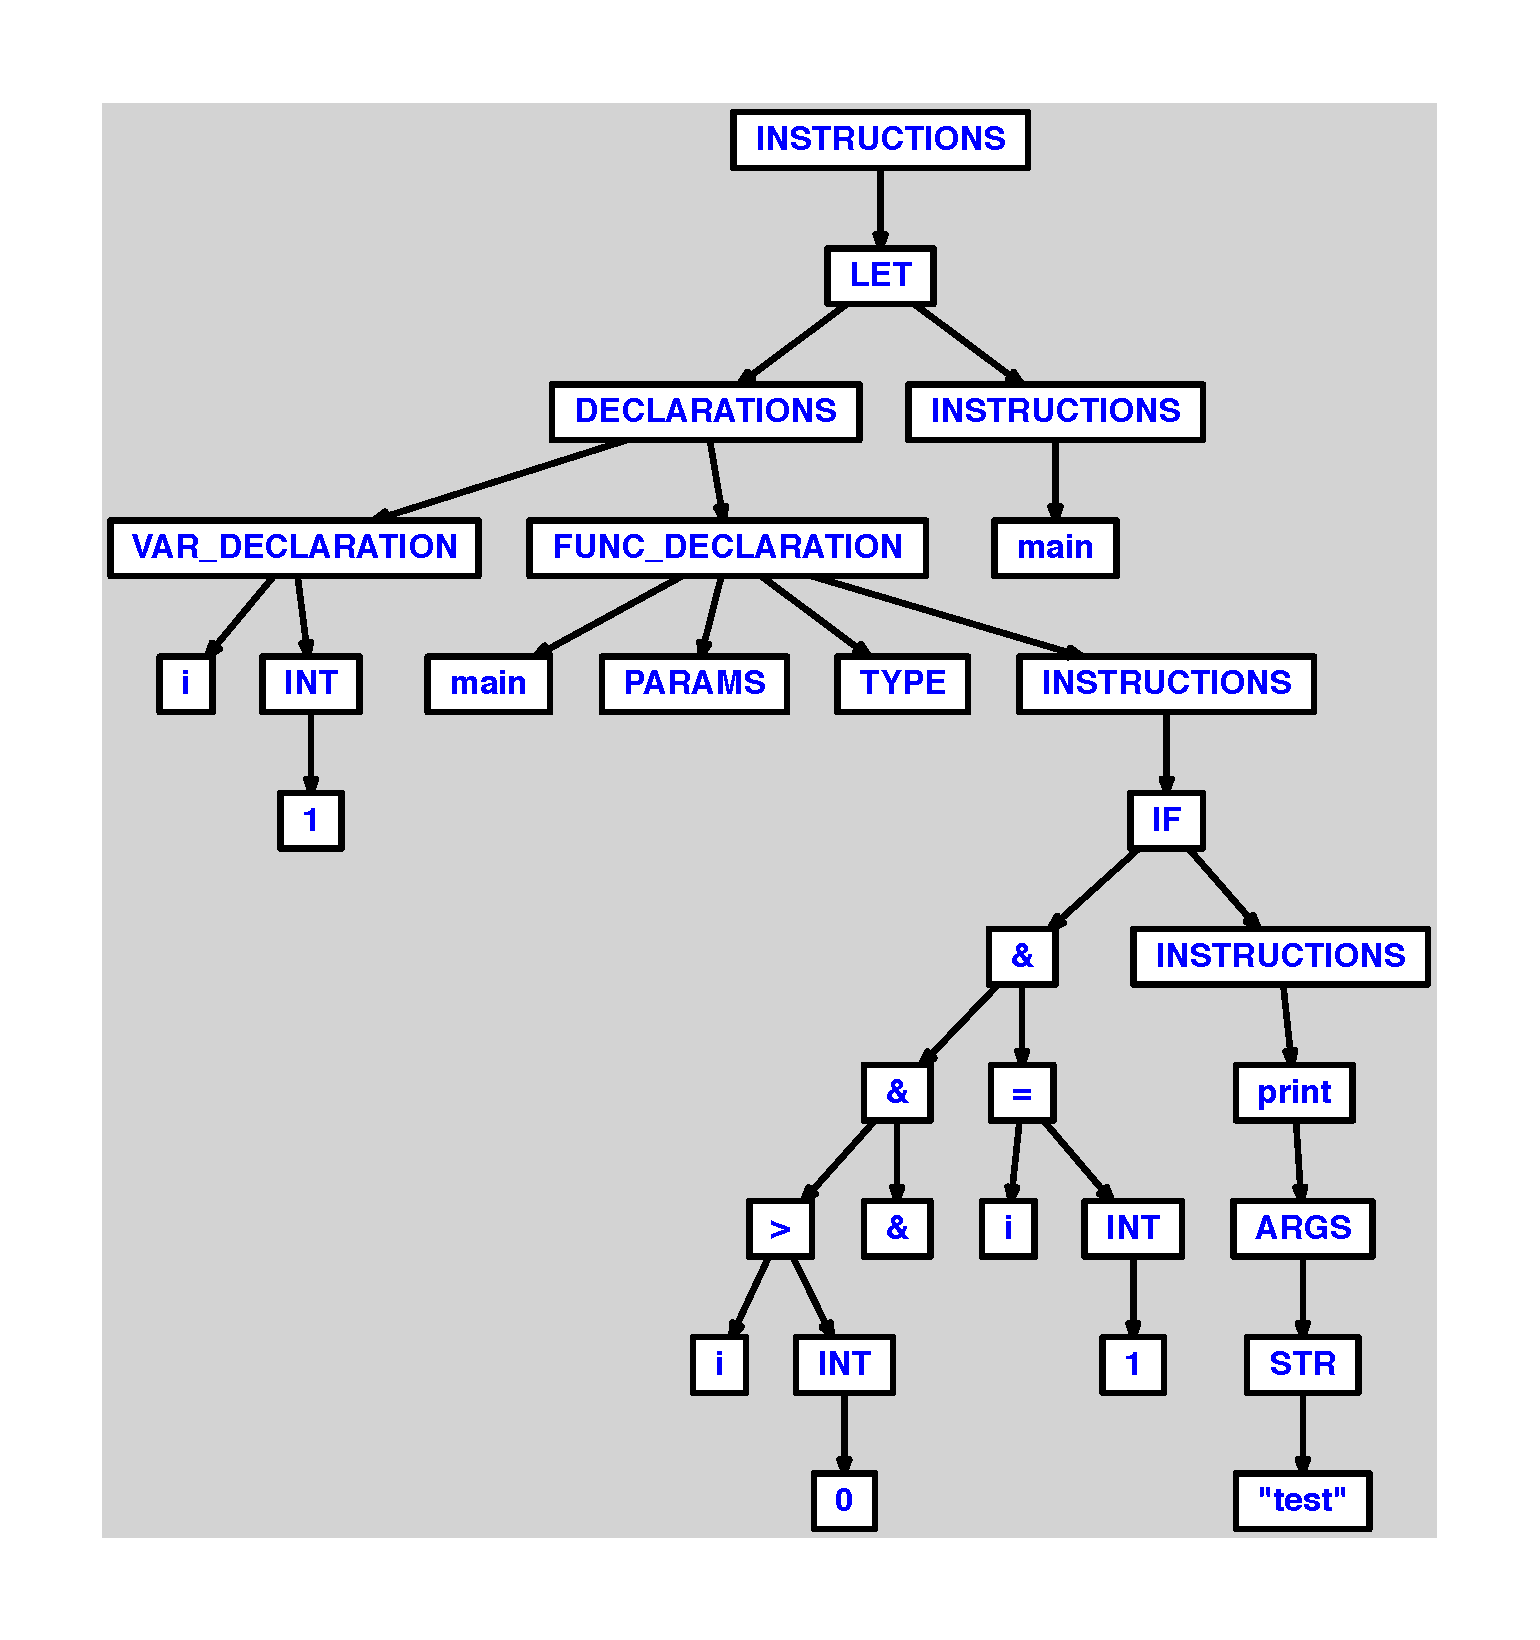
\includegraphics[max width=\textwidth]{ast/ast_0.pdf}\end{figure}\subsection{OK}
\subsubsection{condition avec 1 $ \& $}
\begin{verbatimtab}
let
	var v := 1

	function main() =
		if v > 0 & v < 3 then print("OK")
in main() end
\end{verbatimtab}
\begin{figure}[H]\centering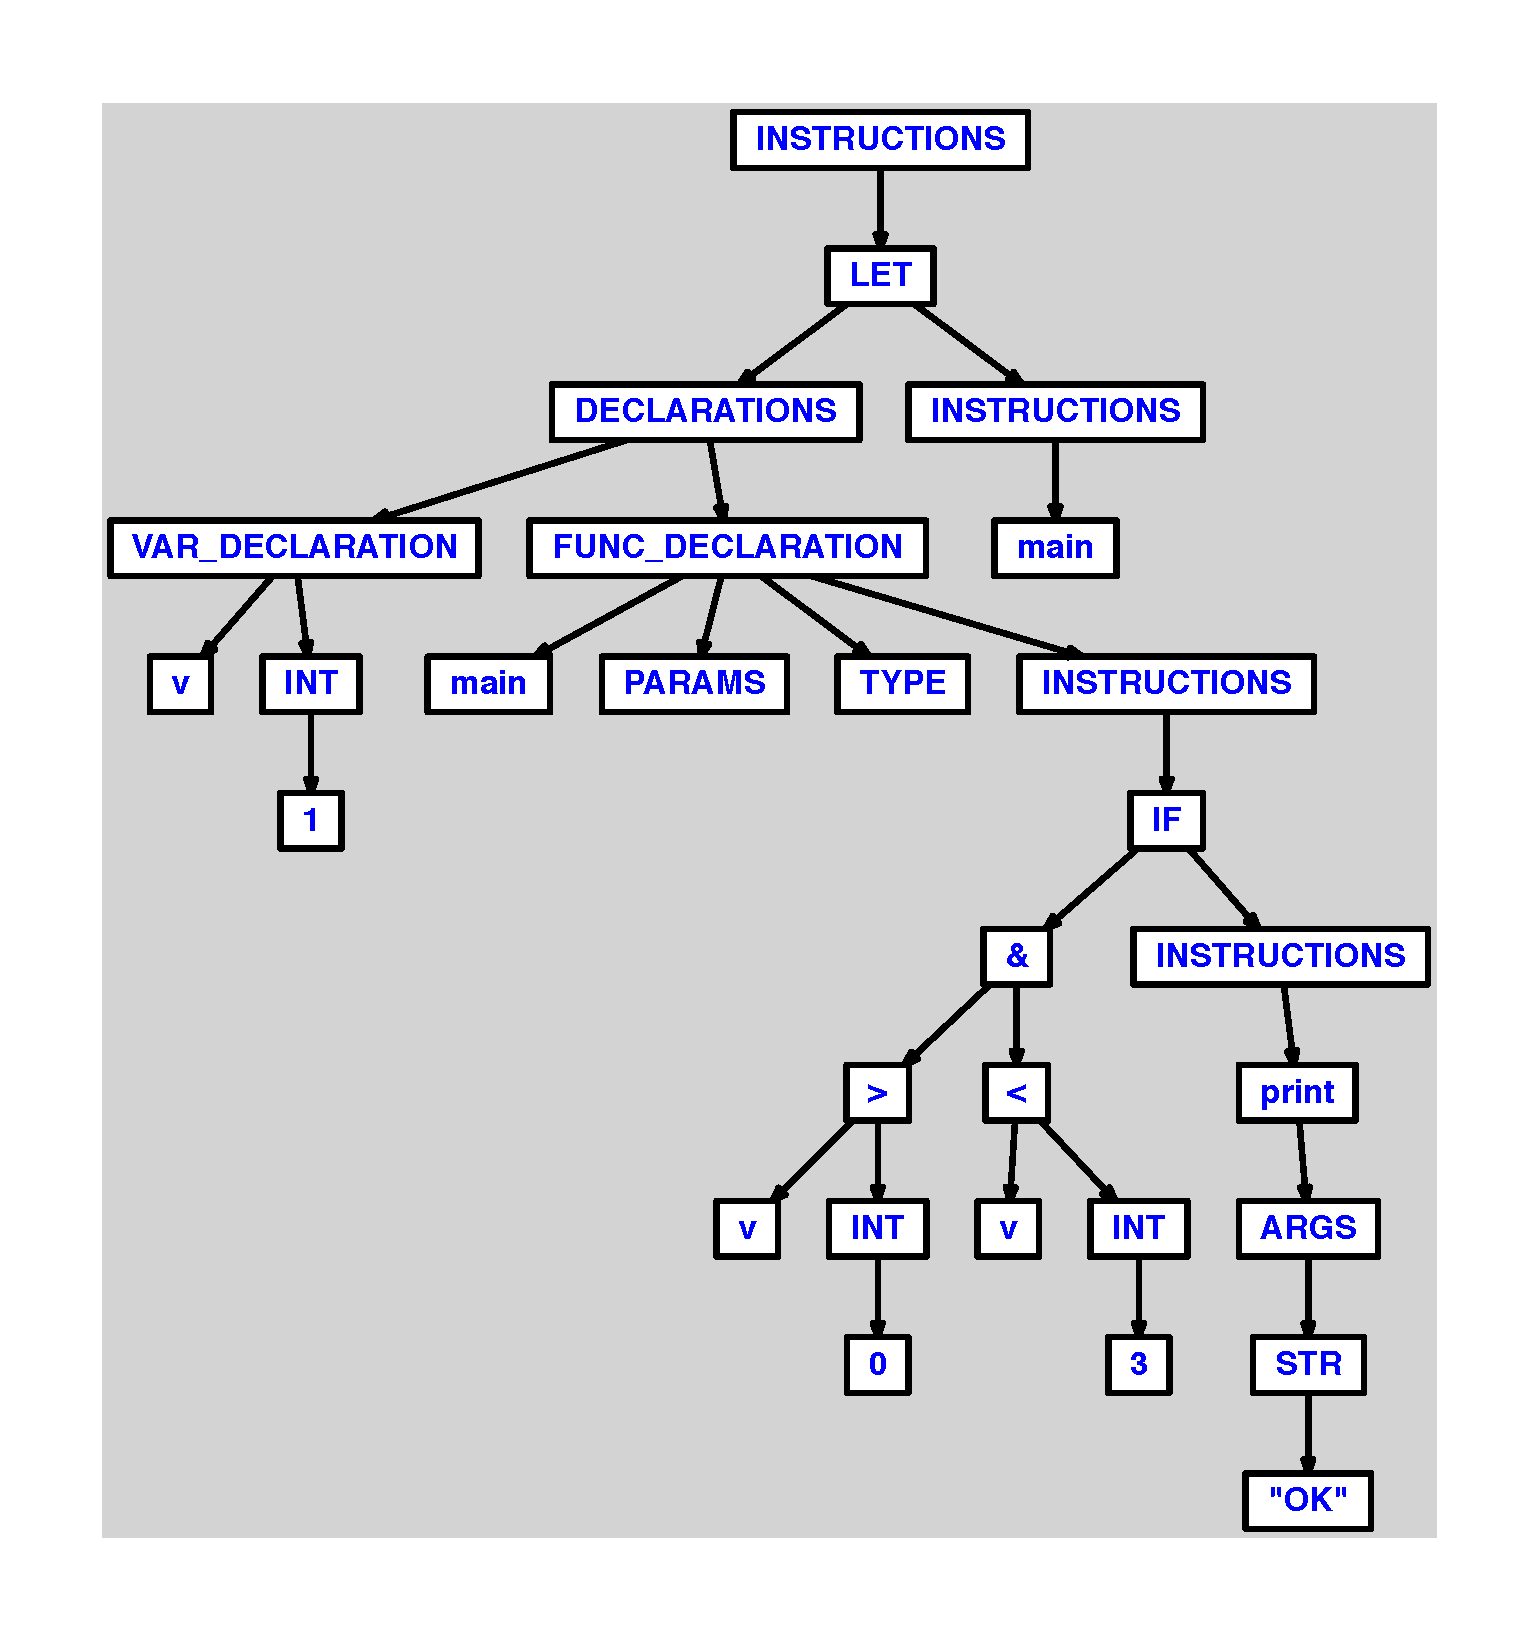
\includegraphics[max width=\textwidth]{ast/ast_1.pdf}\end{figure}\subsubsection{condition avec 2 $ \& $}
\begin{verbatimtab}
let
	var v := 2

	function main() =
		if v > 0 & v < 3 & v/2 = 1 then print("OK")
in main() end
\end{verbatimtab}
\begin{figure}[H]\centering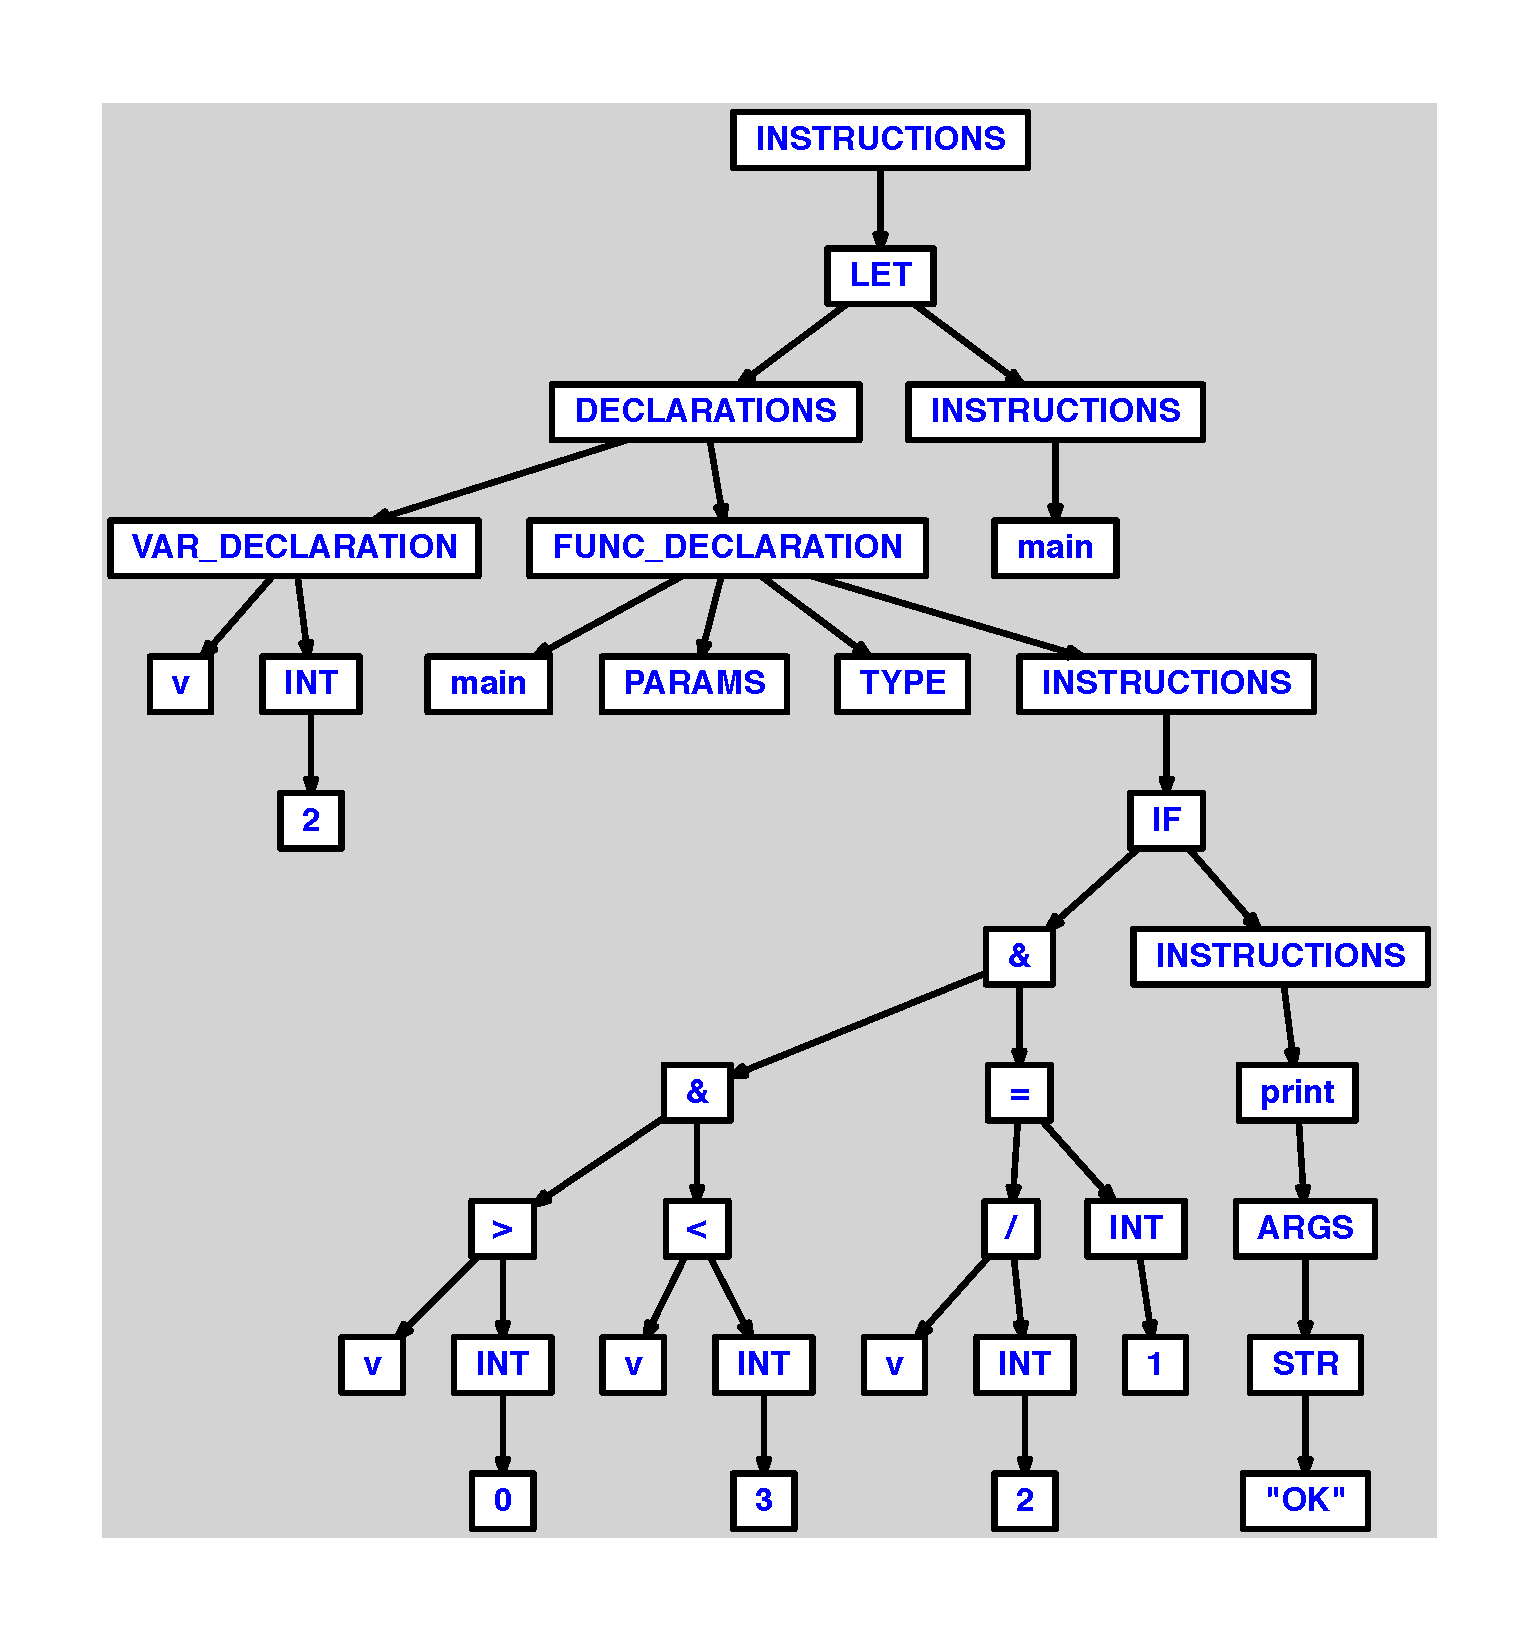
\includegraphics[max width=\textwidth]{ast/ast_2.pdf}\end{figure}\subsubsection{condition avec 3 $ \& $}
\begin{verbatimtab}
let
	var v := 2

	function main() =
		if v > 0 & v < 3 & v/2 = 1 & v-1 = 1 then print("OK")
in main() end
\end{verbatimtab}
\begin{figure}[H]\centering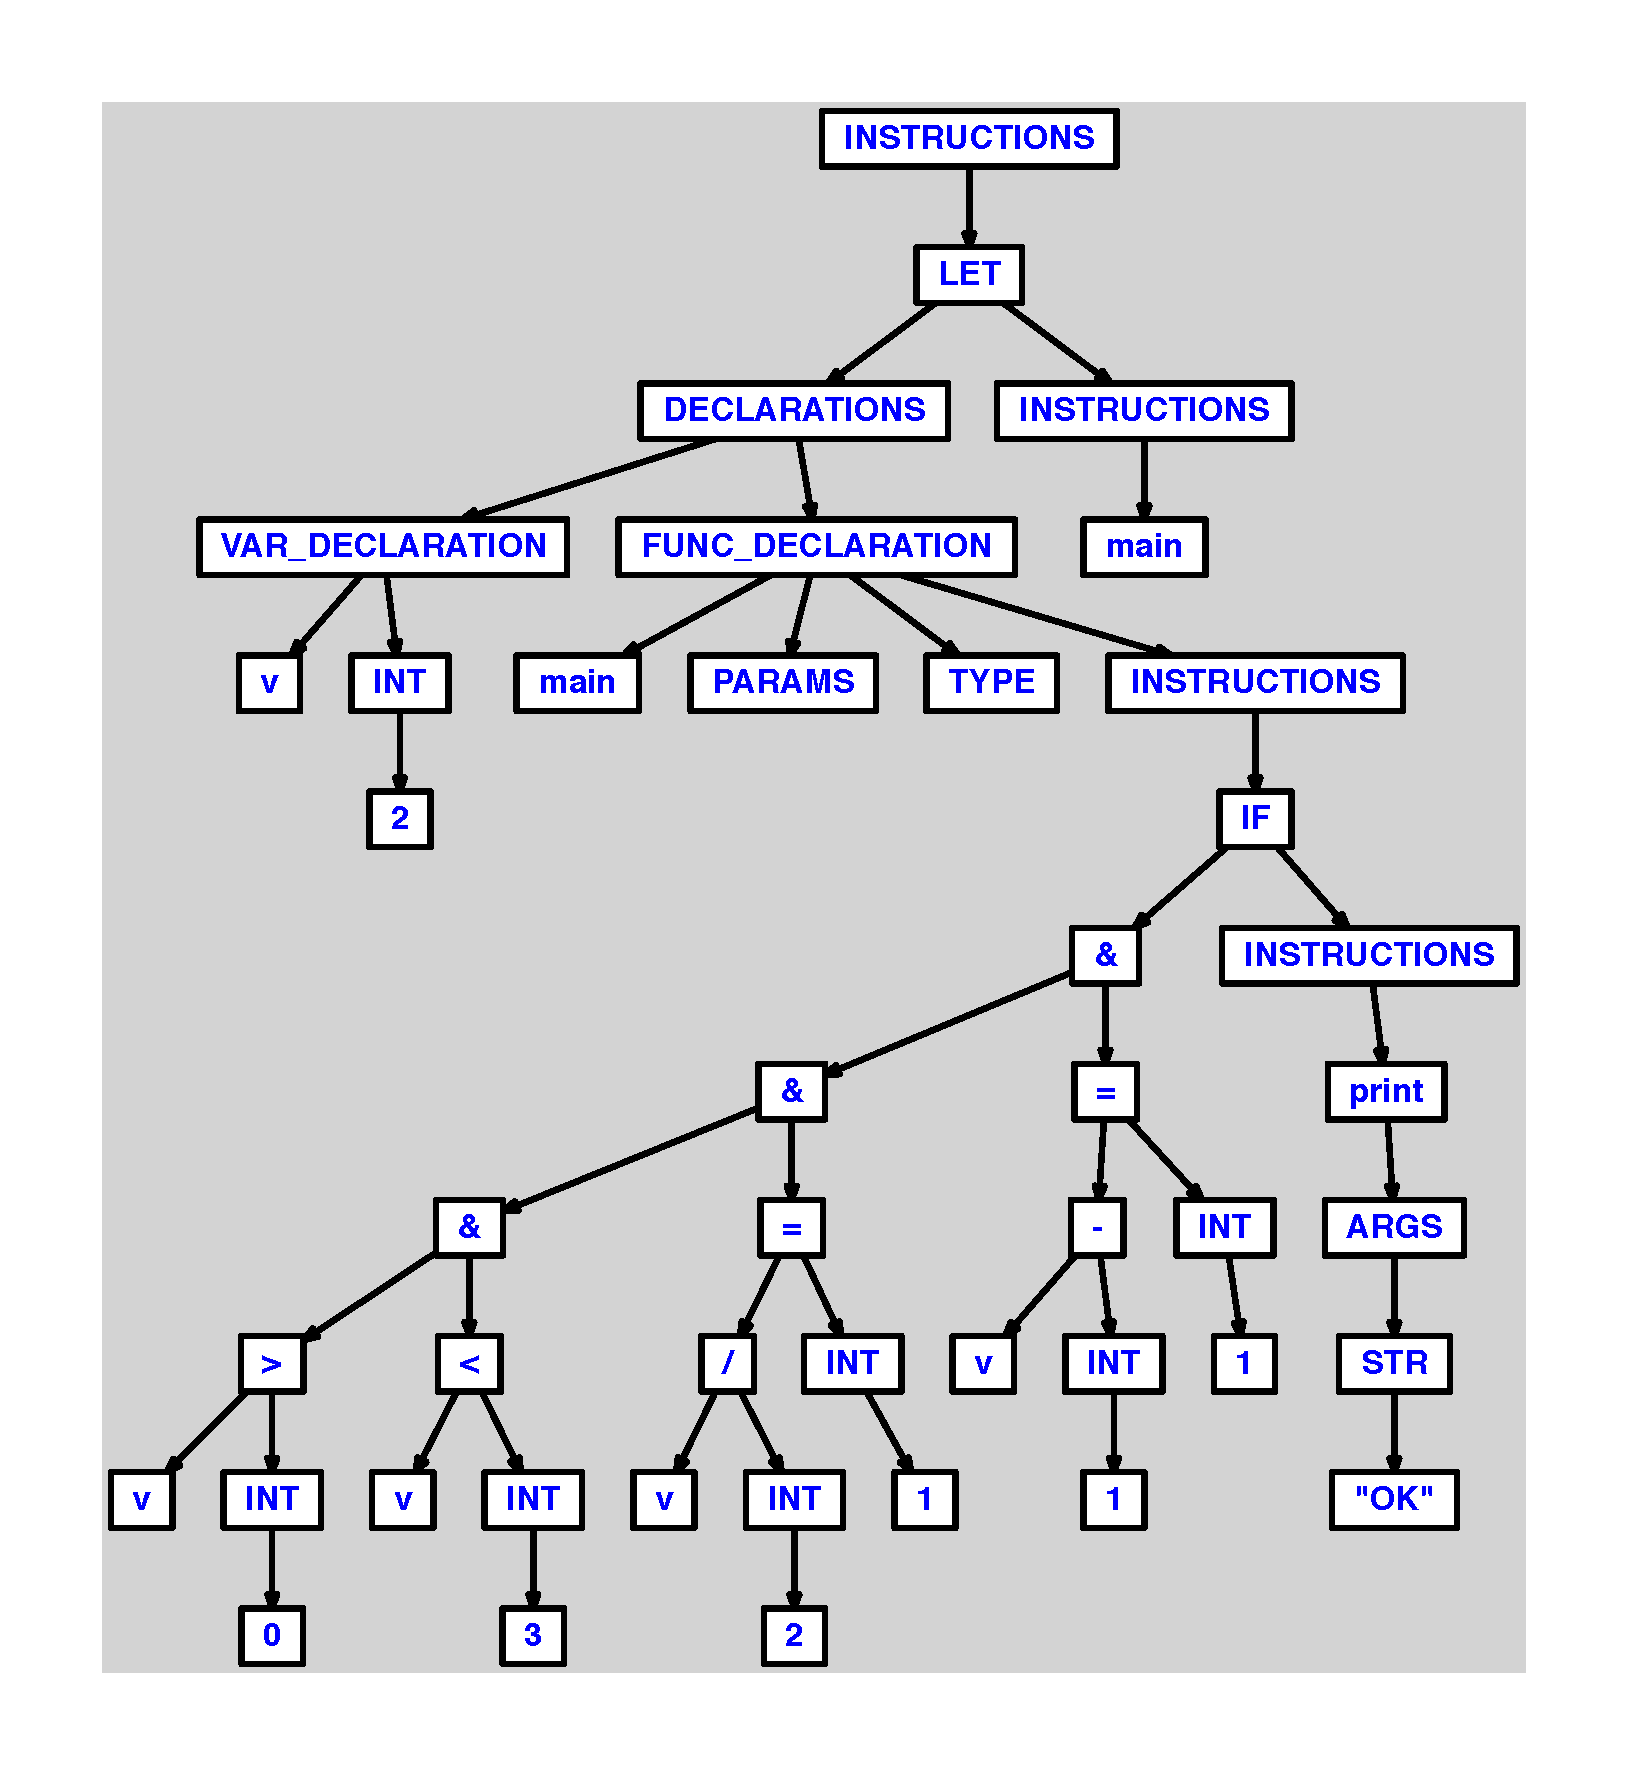
\includegraphics[max width=\textwidth]{ast/ast_3.pdf}\end{figure}\subsubsection{condition avec 2 $ \& $ et 1 $ | $}
\begin{verbatimtab}
let
	var v := 1

	function main() =
		if v/2 > 0 & v <> 1 | v < 5 & v = 1 then print("OK")
in main() end
\end{verbatimtab}
\begin{figure}[H]\centering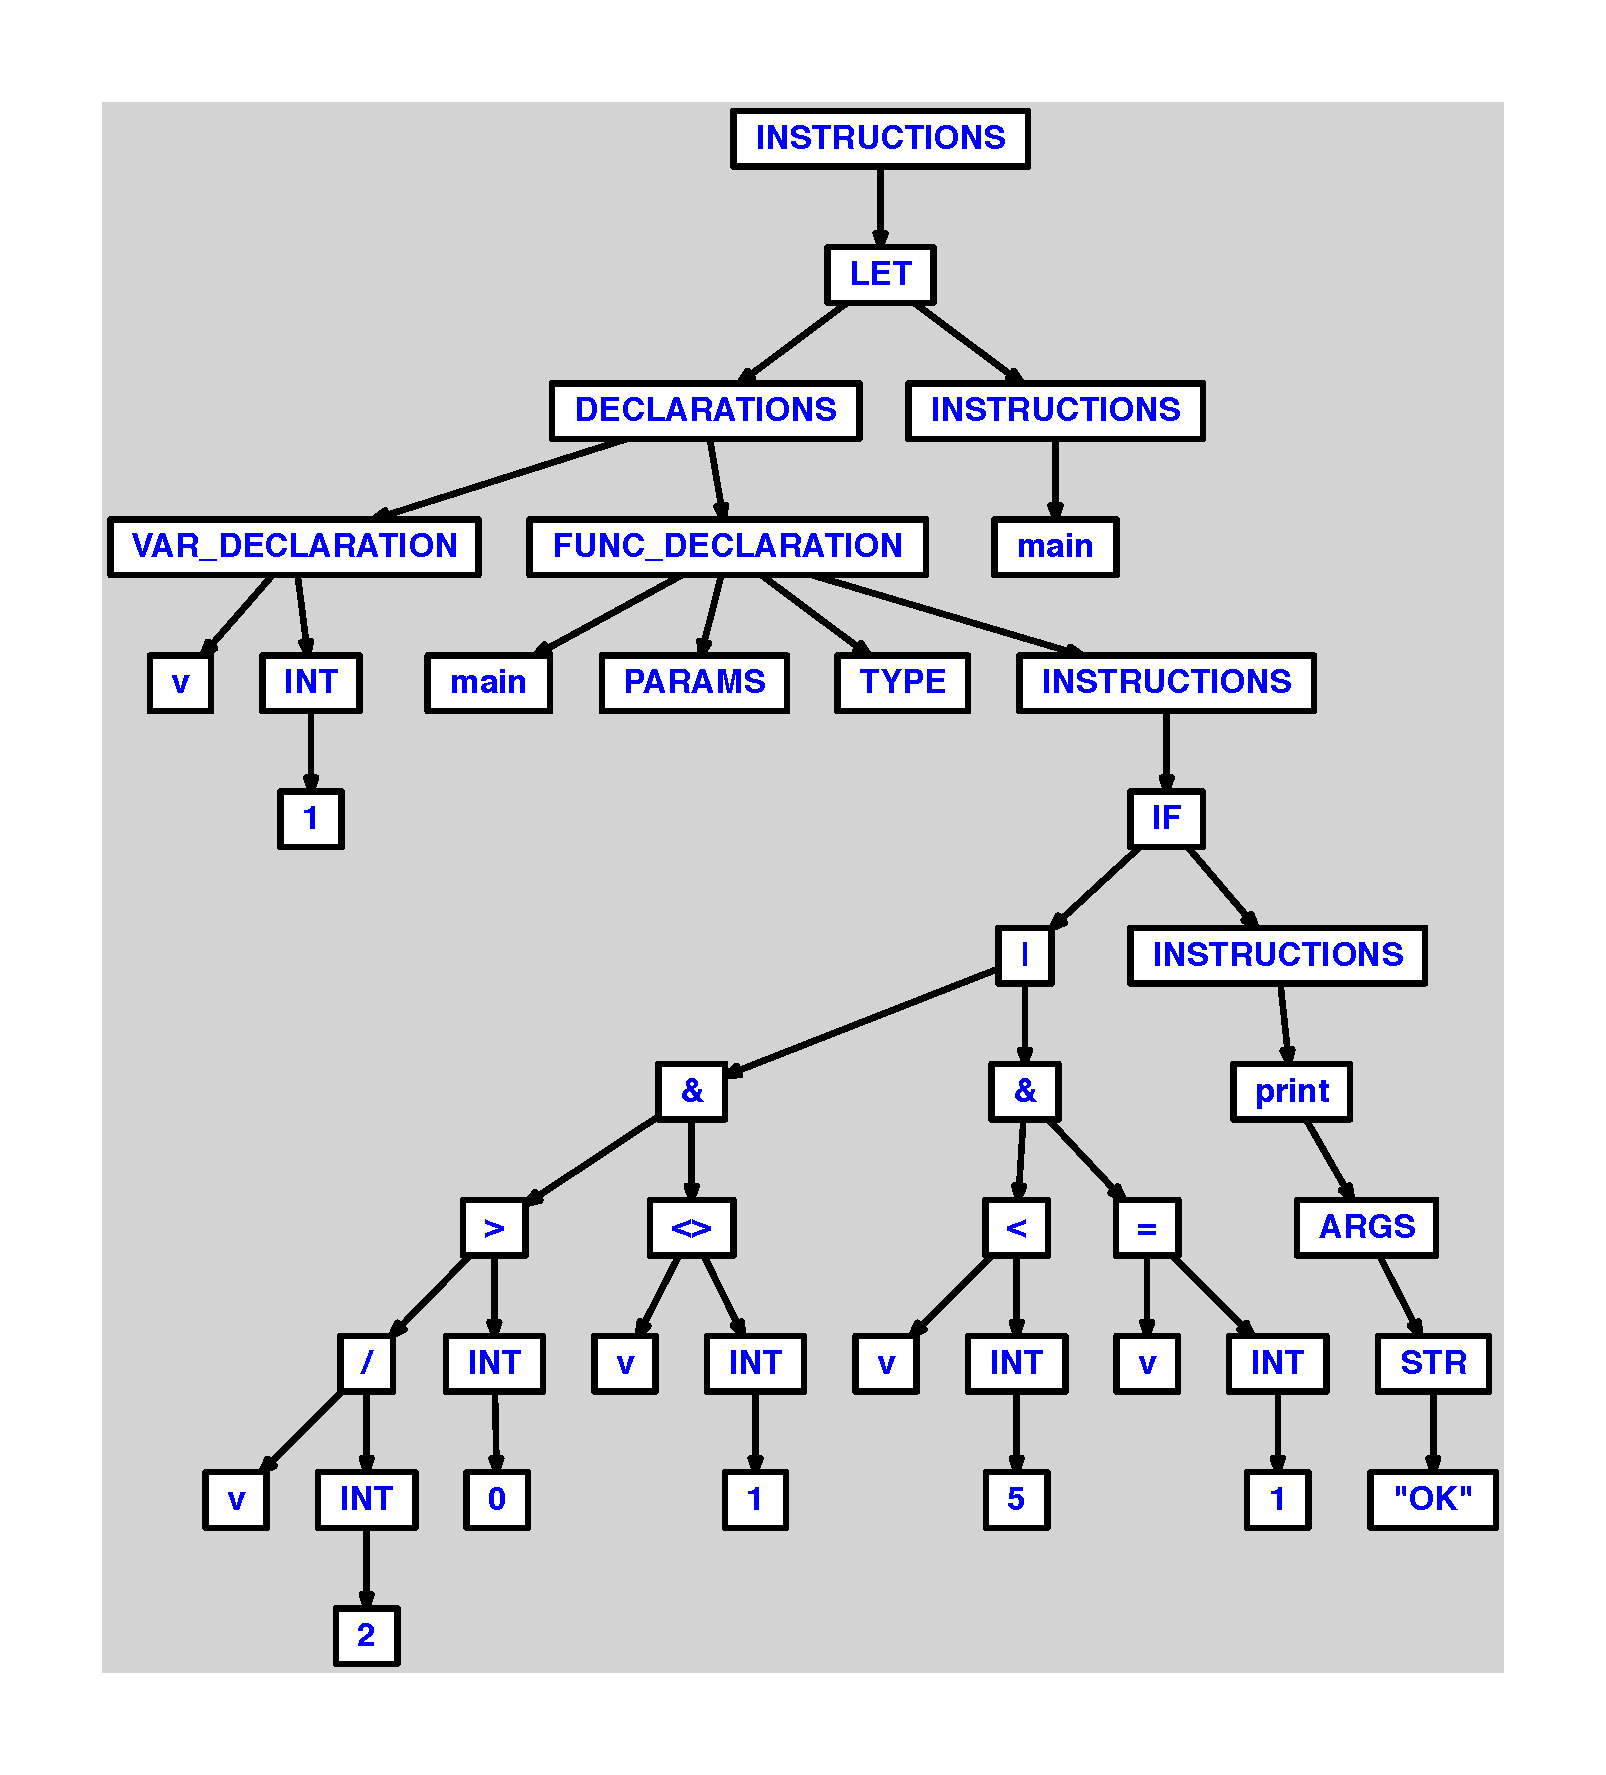
\includegraphics[max width=\textwidth]{ast/ast_4.pdf}\end{figure}\subsubsection{$ \& $ avec des entiers}
\begin{verbatimtab}
let
	function main() =
		if 1 & 1 then print("test")
in main() end
\end{verbatimtab}
\begin{figure}[H]\centering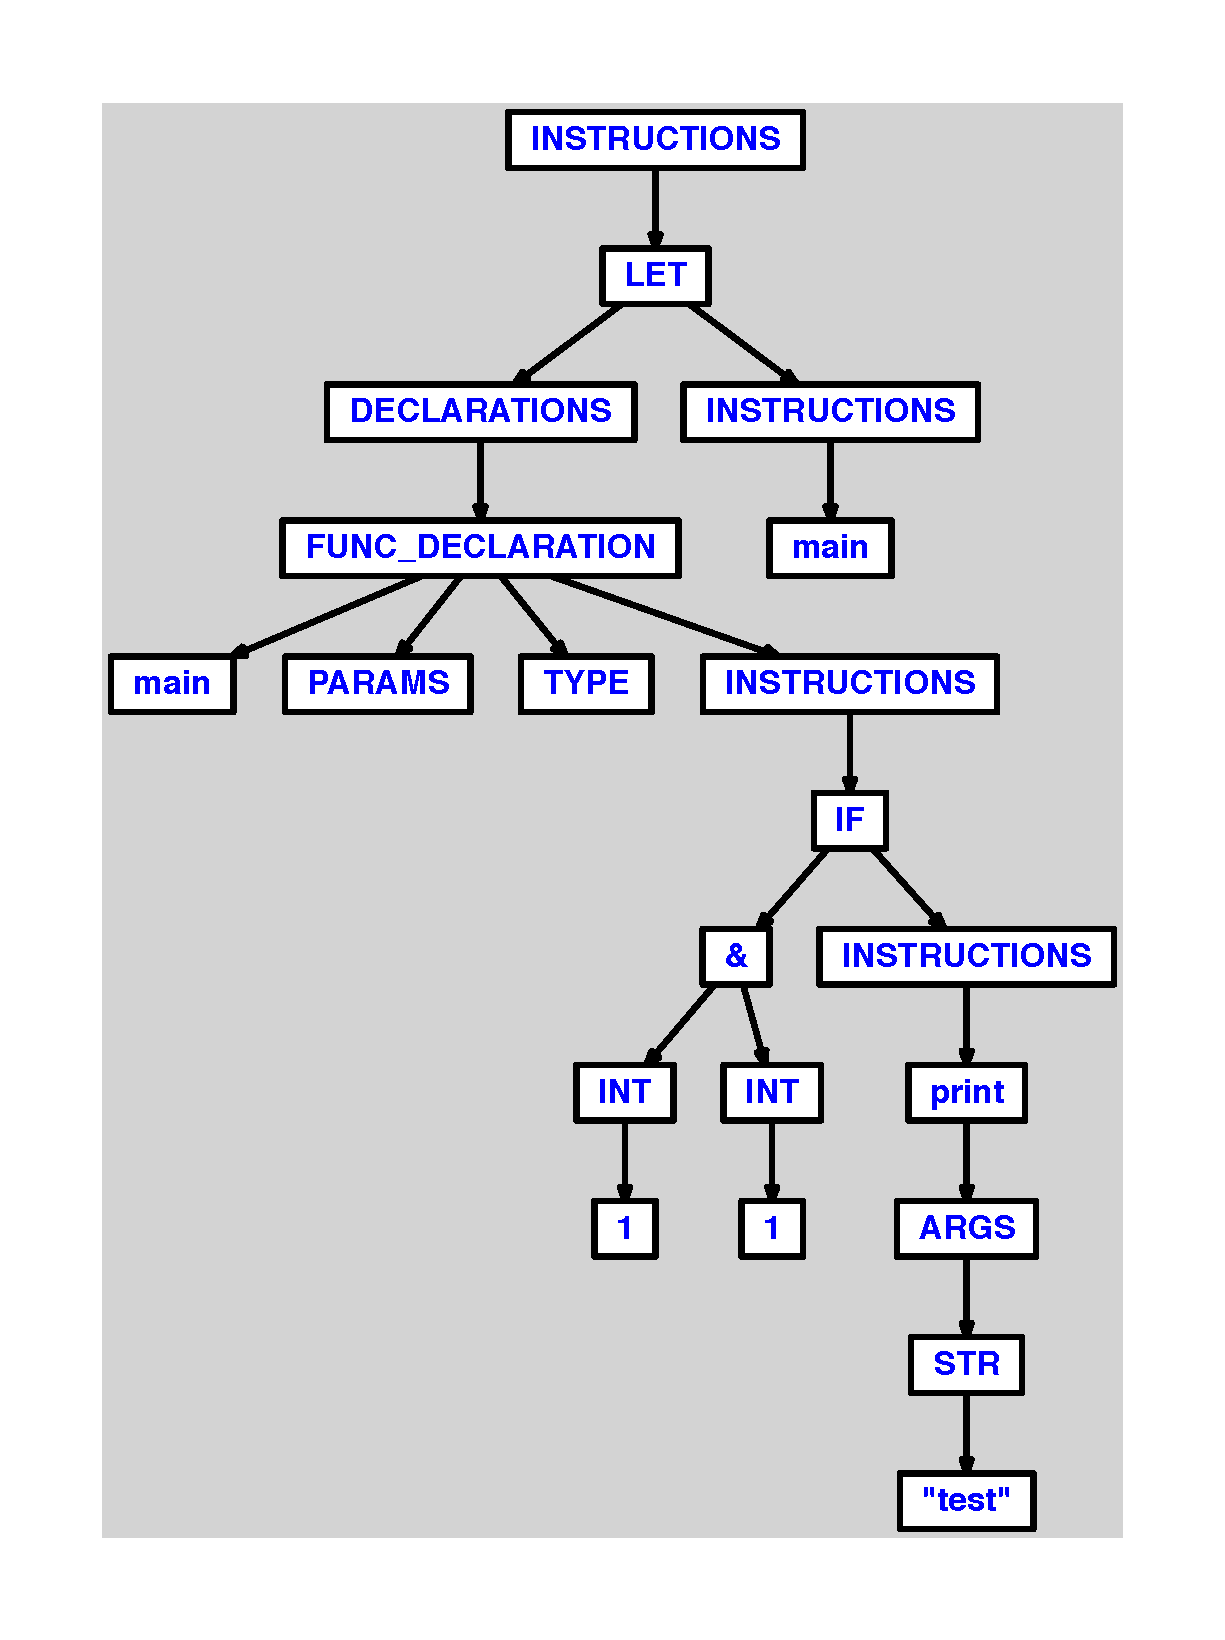
\includegraphics[max width=\textwidth]{ast/ast_5.pdf}\end{figure}\subsubsection{$ \& $ avec des chaines}
\begin{verbatimtab}
let
	function main() =
		if "test" & "test" then print("test")
in main() end
\end{verbatimtab}
\begin{figure}[H]\centering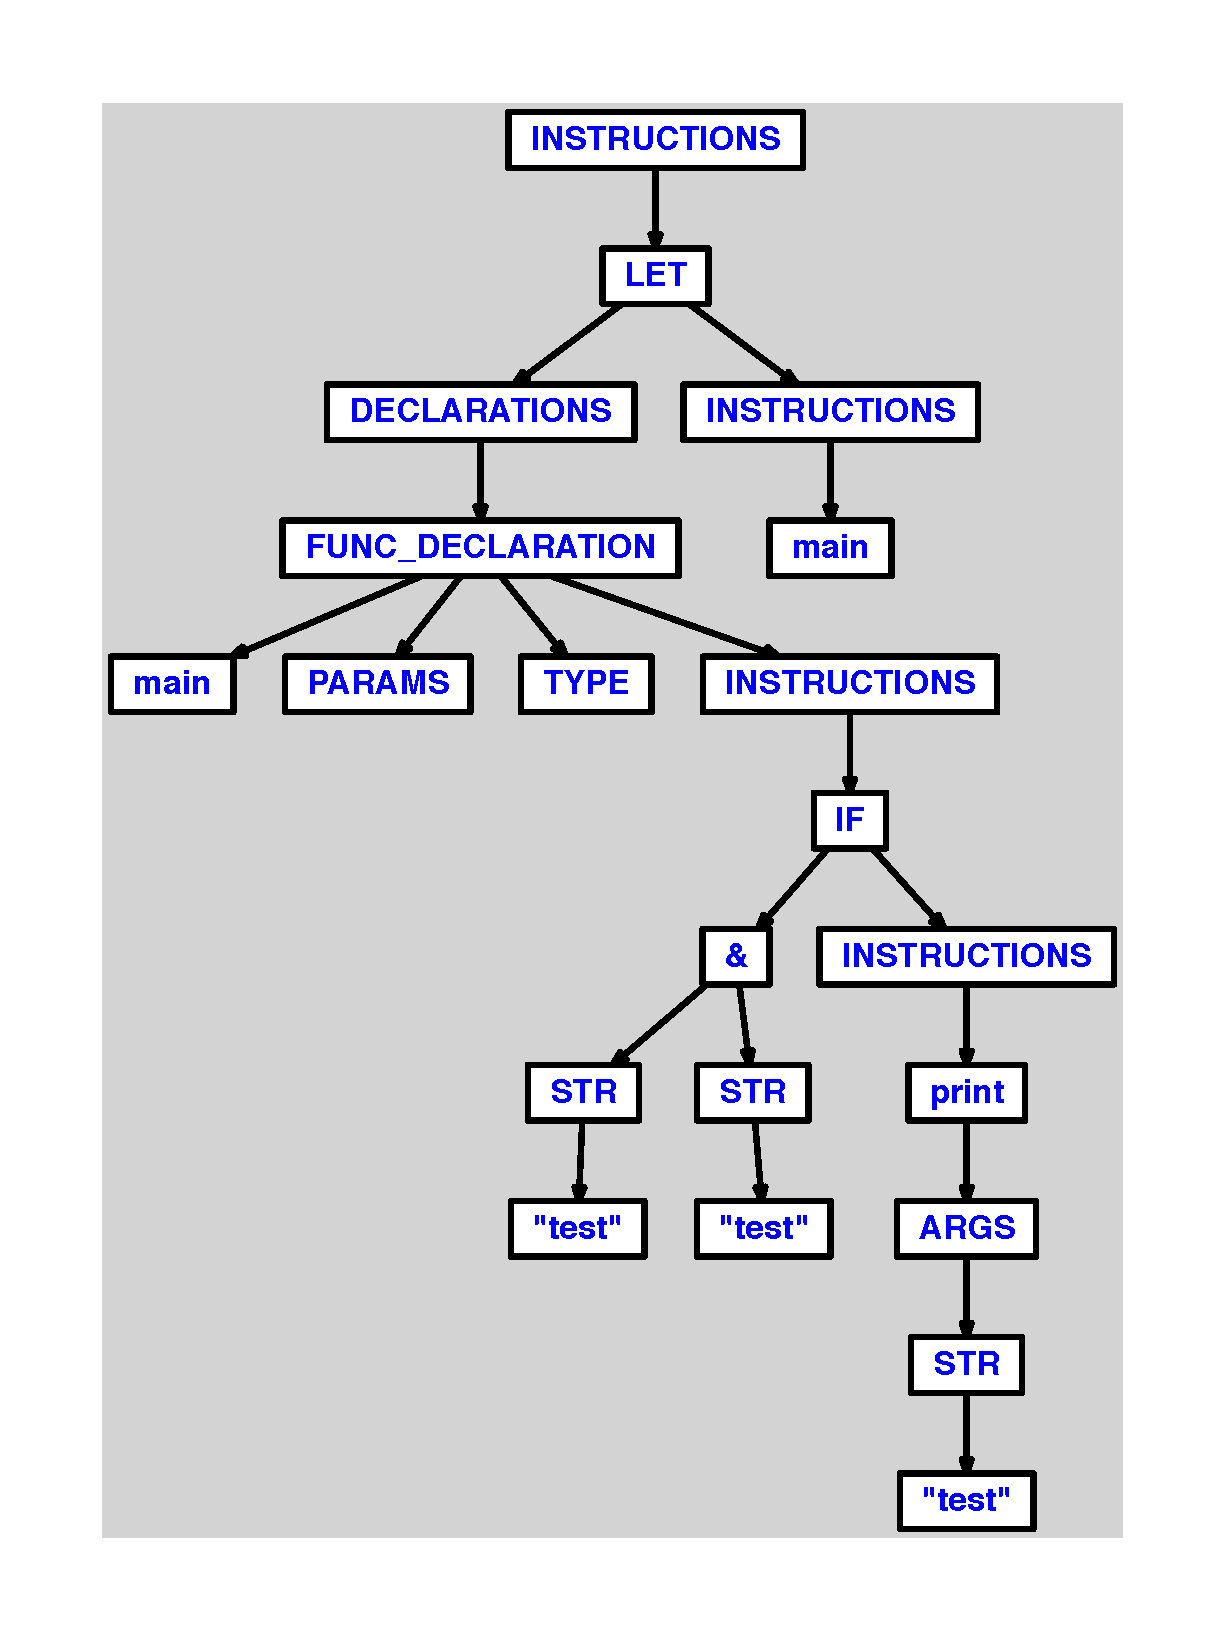
\includegraphics[max width=\textwidth]{ast/ast_6.pdf}\end{figure}\section{break}
\subsection{KO}
\subsubsection{break comme condition dans if}
\begin{verbatimtab}
let
	function main() =
		if break then
			print("test")
in main() end
\end{verbatimtab}
\begin{figure}[H]\centering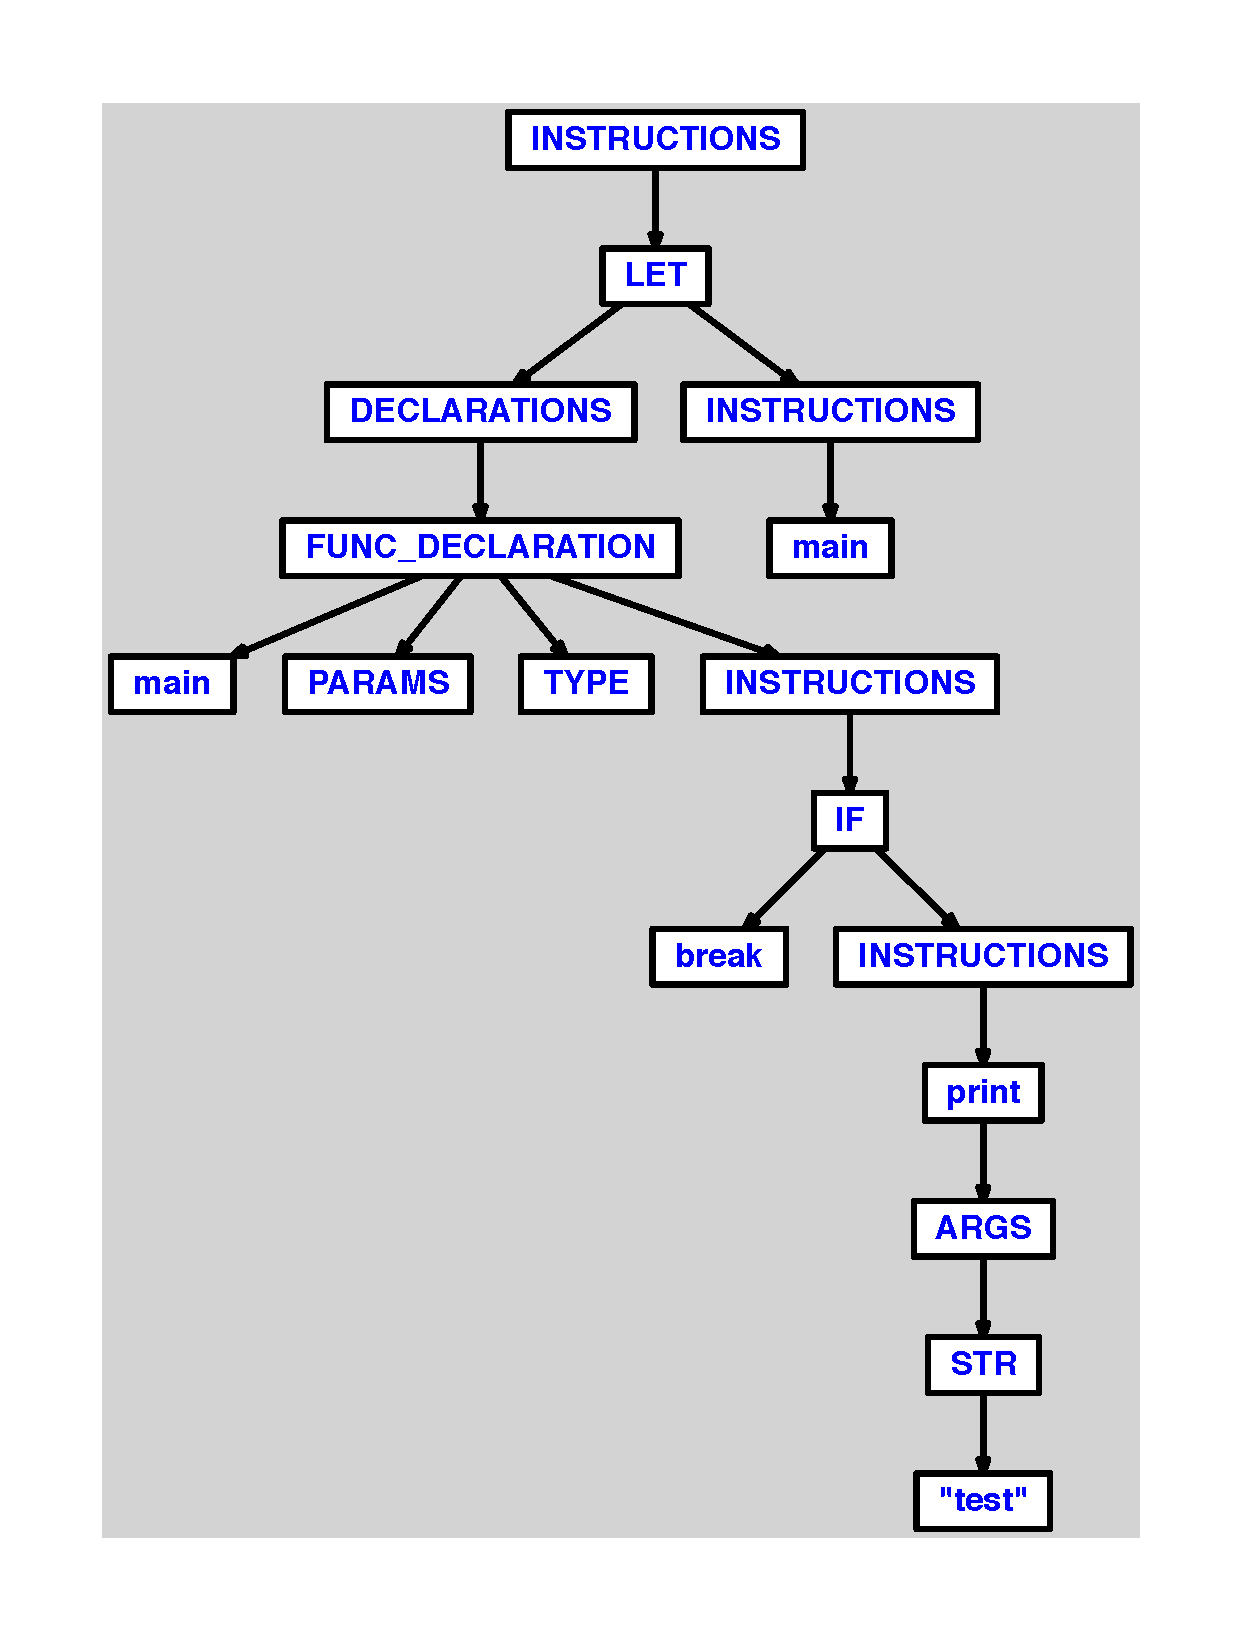
\includegraphics[max width=\textwidth]{ast/ast_7.pdf}\end{figure}\subsubsection{break comme condition dans while}
\begin{verbatimtab}
let
	function main() =
		while break then
			print("test")
in main() end
\end{verbatimtab}
\subsection{OK}
\subsubsection{break dans un for, apres instruction}
\begin{verbatimtab}
let
	function main() =
		for i := 0 to 3 do
			print("test");
			break
in main() end
\end{verbatimtab}
\begin{figure}[H]\centering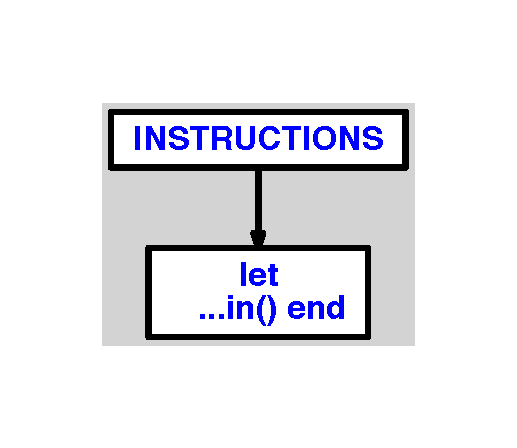
\includegraphics[max width=\textwidth]{ast/ast_9.pdf}\end{figure}\subsubsection{break dans un for, sans instruction avant}
\begin{verbatimtab}
let
	function main() =
		for i := 0 to 3 do
			break
in main() end
\end{verbatimtab}
\begin{figure}[H]\centering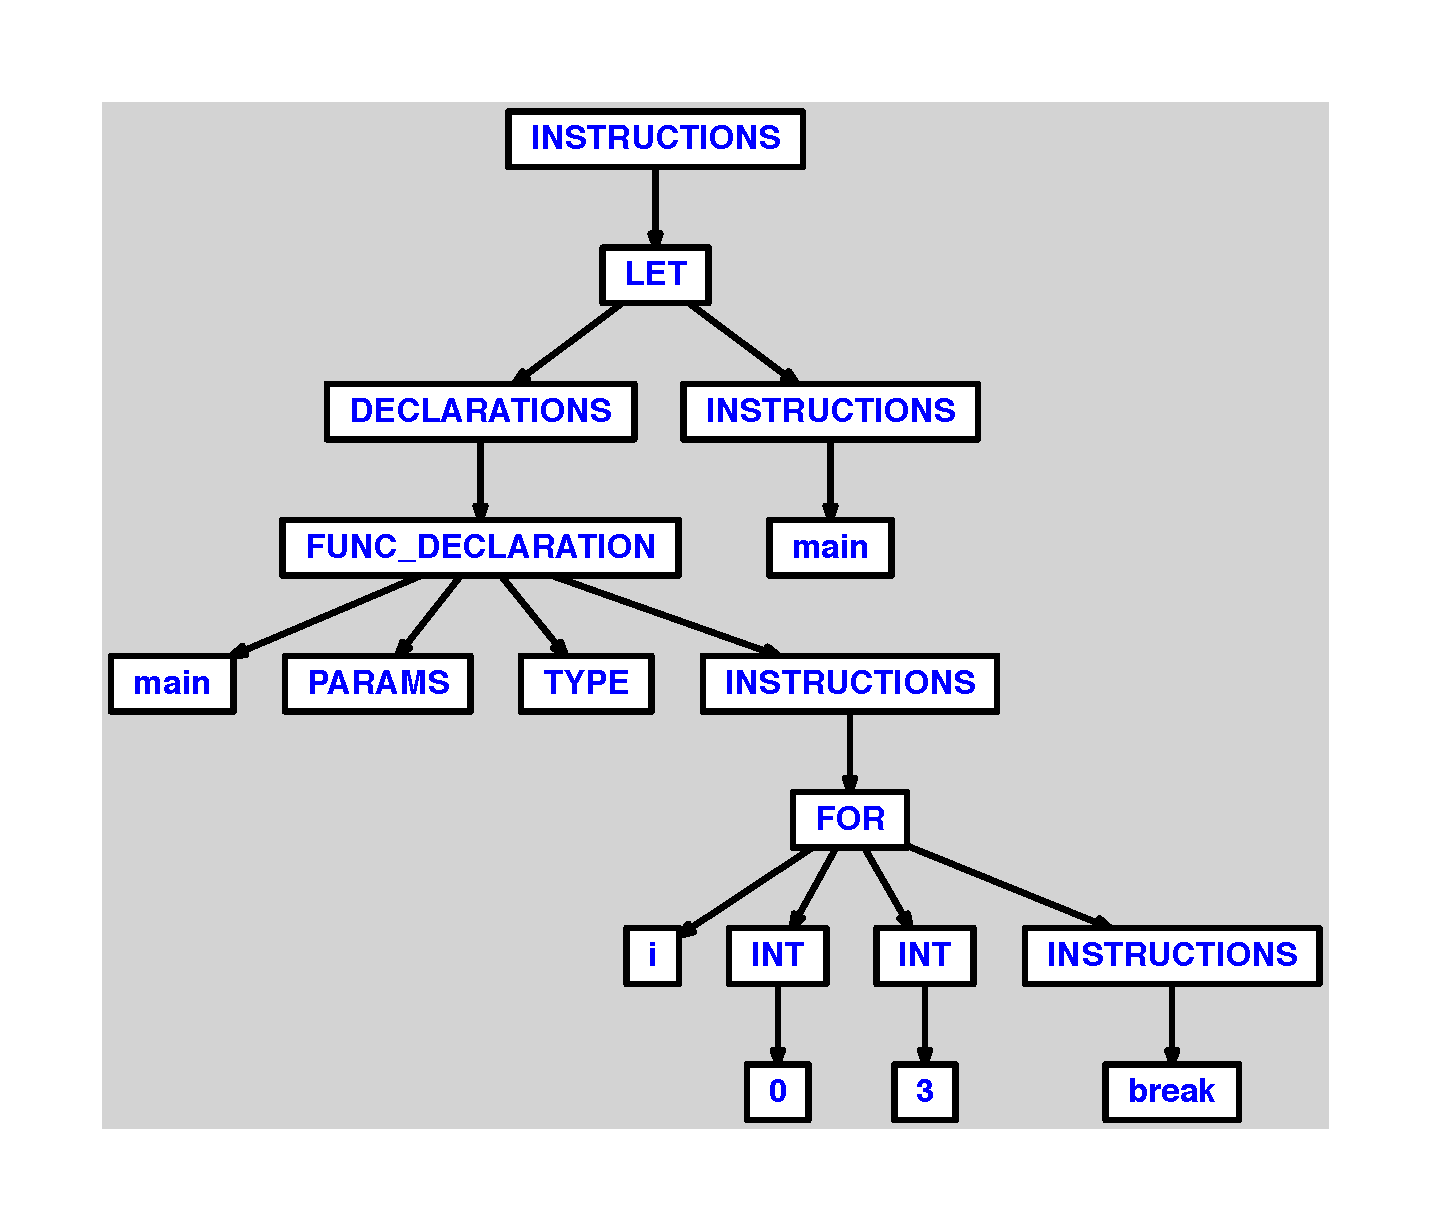
\includegraphics[max width=\textwidth]{ast/ast_10.pdf}\end{figure}\subsubsection{fonction executant seulement break}
\begin{verbatimtab}
let
	function main() = break
in main() end
\end{verbatimtab}
\begin{figure}[H]\centering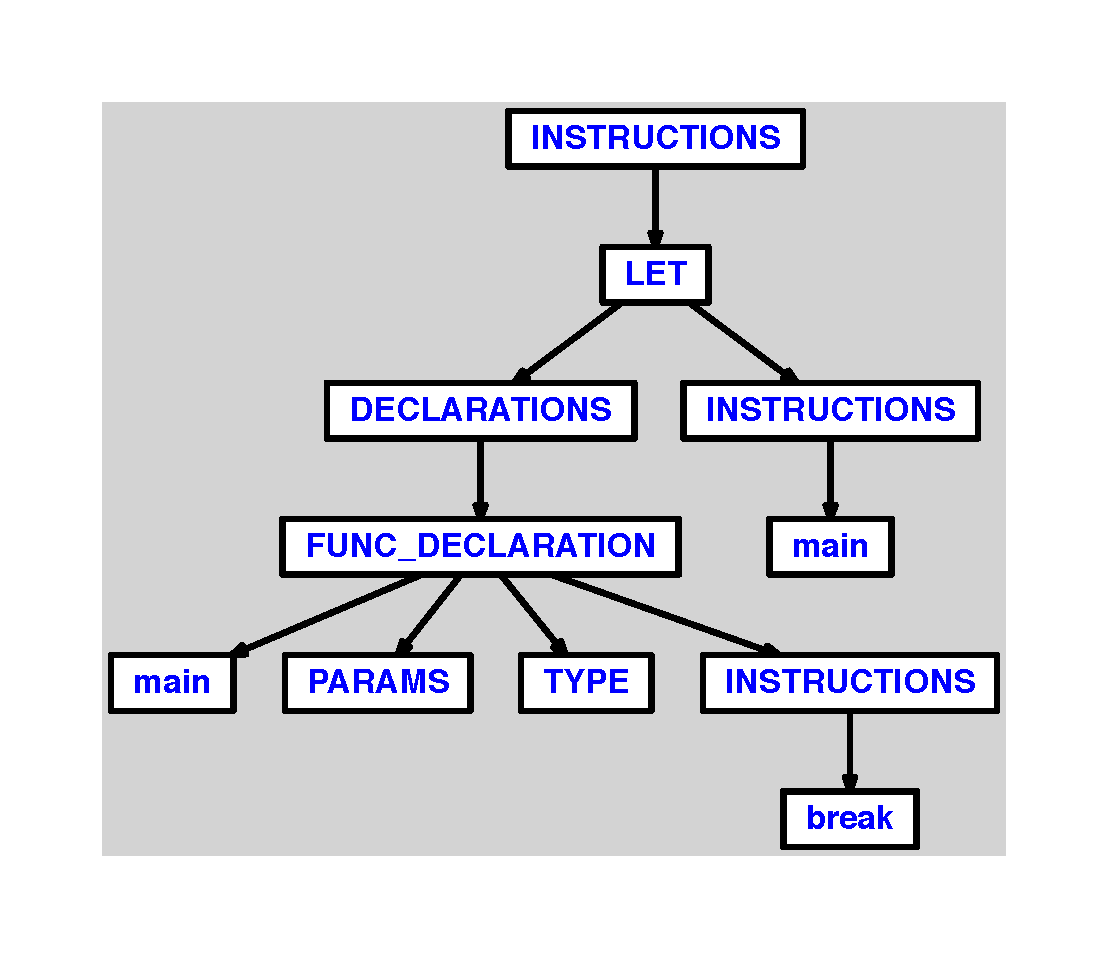
\includegraphics[max width=\textwidth]{ast/ast_11.pdf}\end{figure}\subsubsection{appel de break, avec corps de programme contenant break}
\begin{verbatimtab}
let
	break
in break end
\end{verbatimtab}
\begin{figure}[H]\centering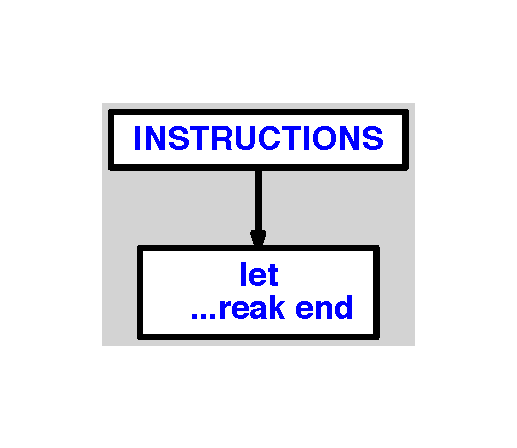
\includegraphics[max width=\textwidth]{ast/ast_12.pdf}\end{figure}\subsubsection{appel de break, avec corps de programme ne contenant pas break}
\begin{verbatimtab}
let
	function main() = print("test")
in break end
\end{verbatimtab}
\begin{figure}[H]\centering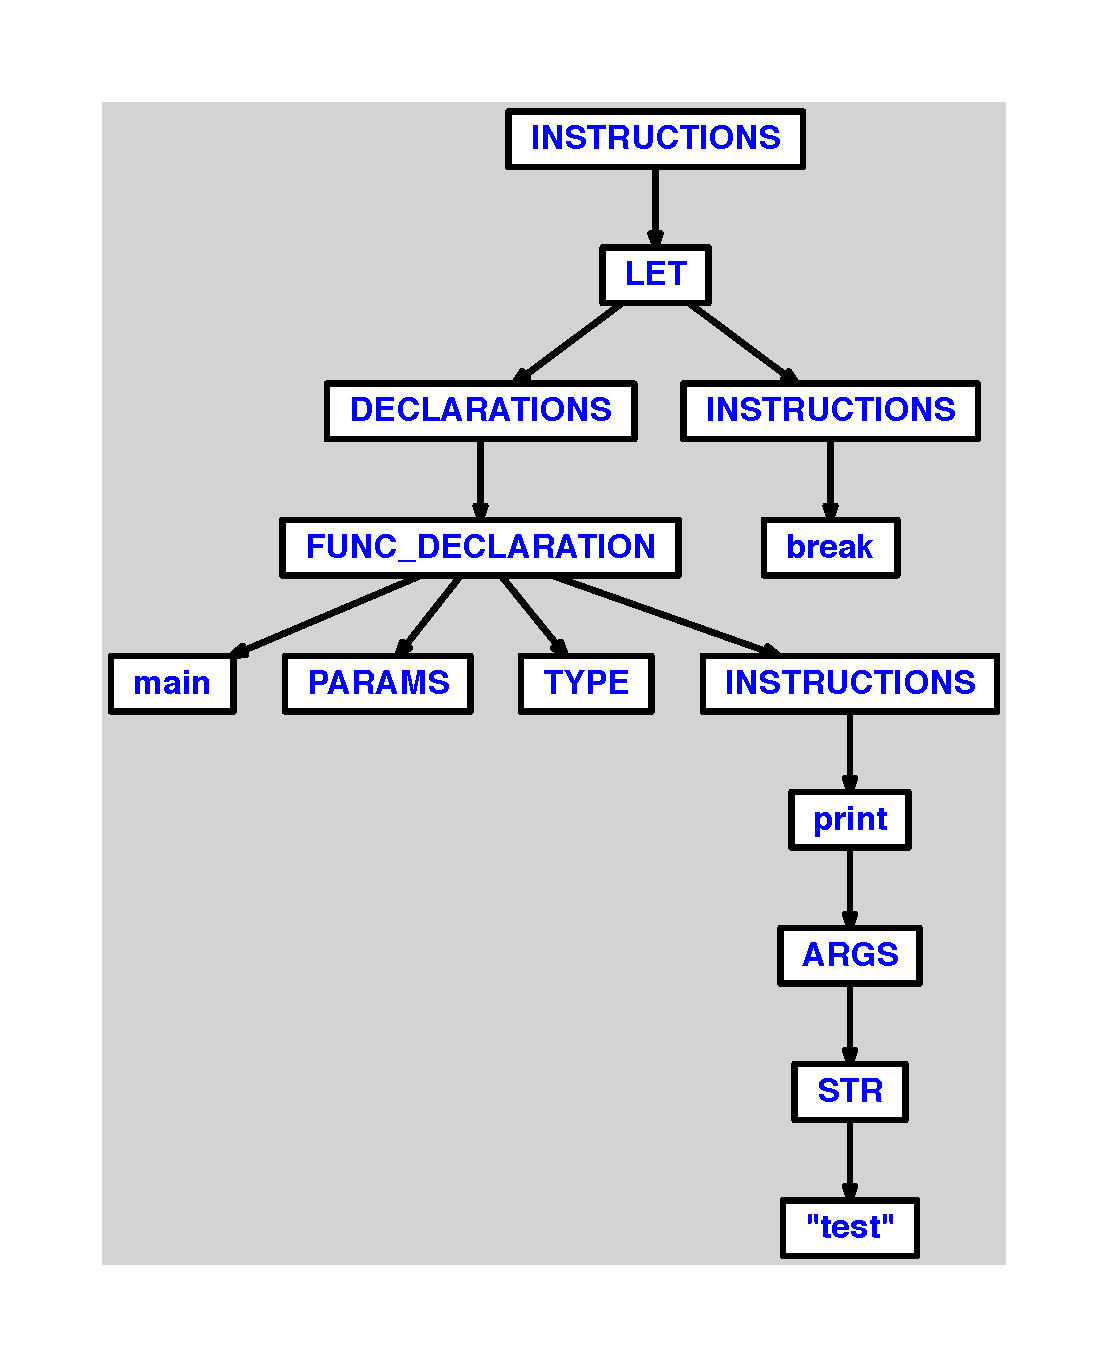
\includegraphics[max width=\textwidth]{ast/ast_13.pdf}\end{figure}\subsubsection{break dans un while, apres instruction}
\begin{verbatimtab}
let
	var i := 3

	function main() =
		while i > 0 do
			print("test");
			break
in main() end
\end{verbatimtab}
\begin{figure}[H]\centering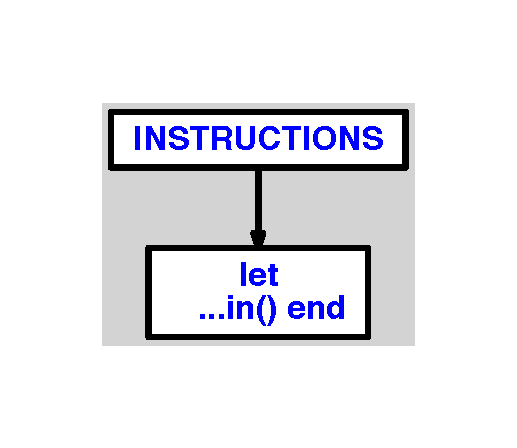
\includegraphics[max width=\textwidth]{ast/ast_14.pdf}\end{figure}\subsubsection{break dans un while, sans instruction avant}
\begin{verbatimtab}
let
	var i := 3

	function main() =
		while i > 0 do
			break
in main() end
\end{verbatimtab}
\begin{figure}[H]\centering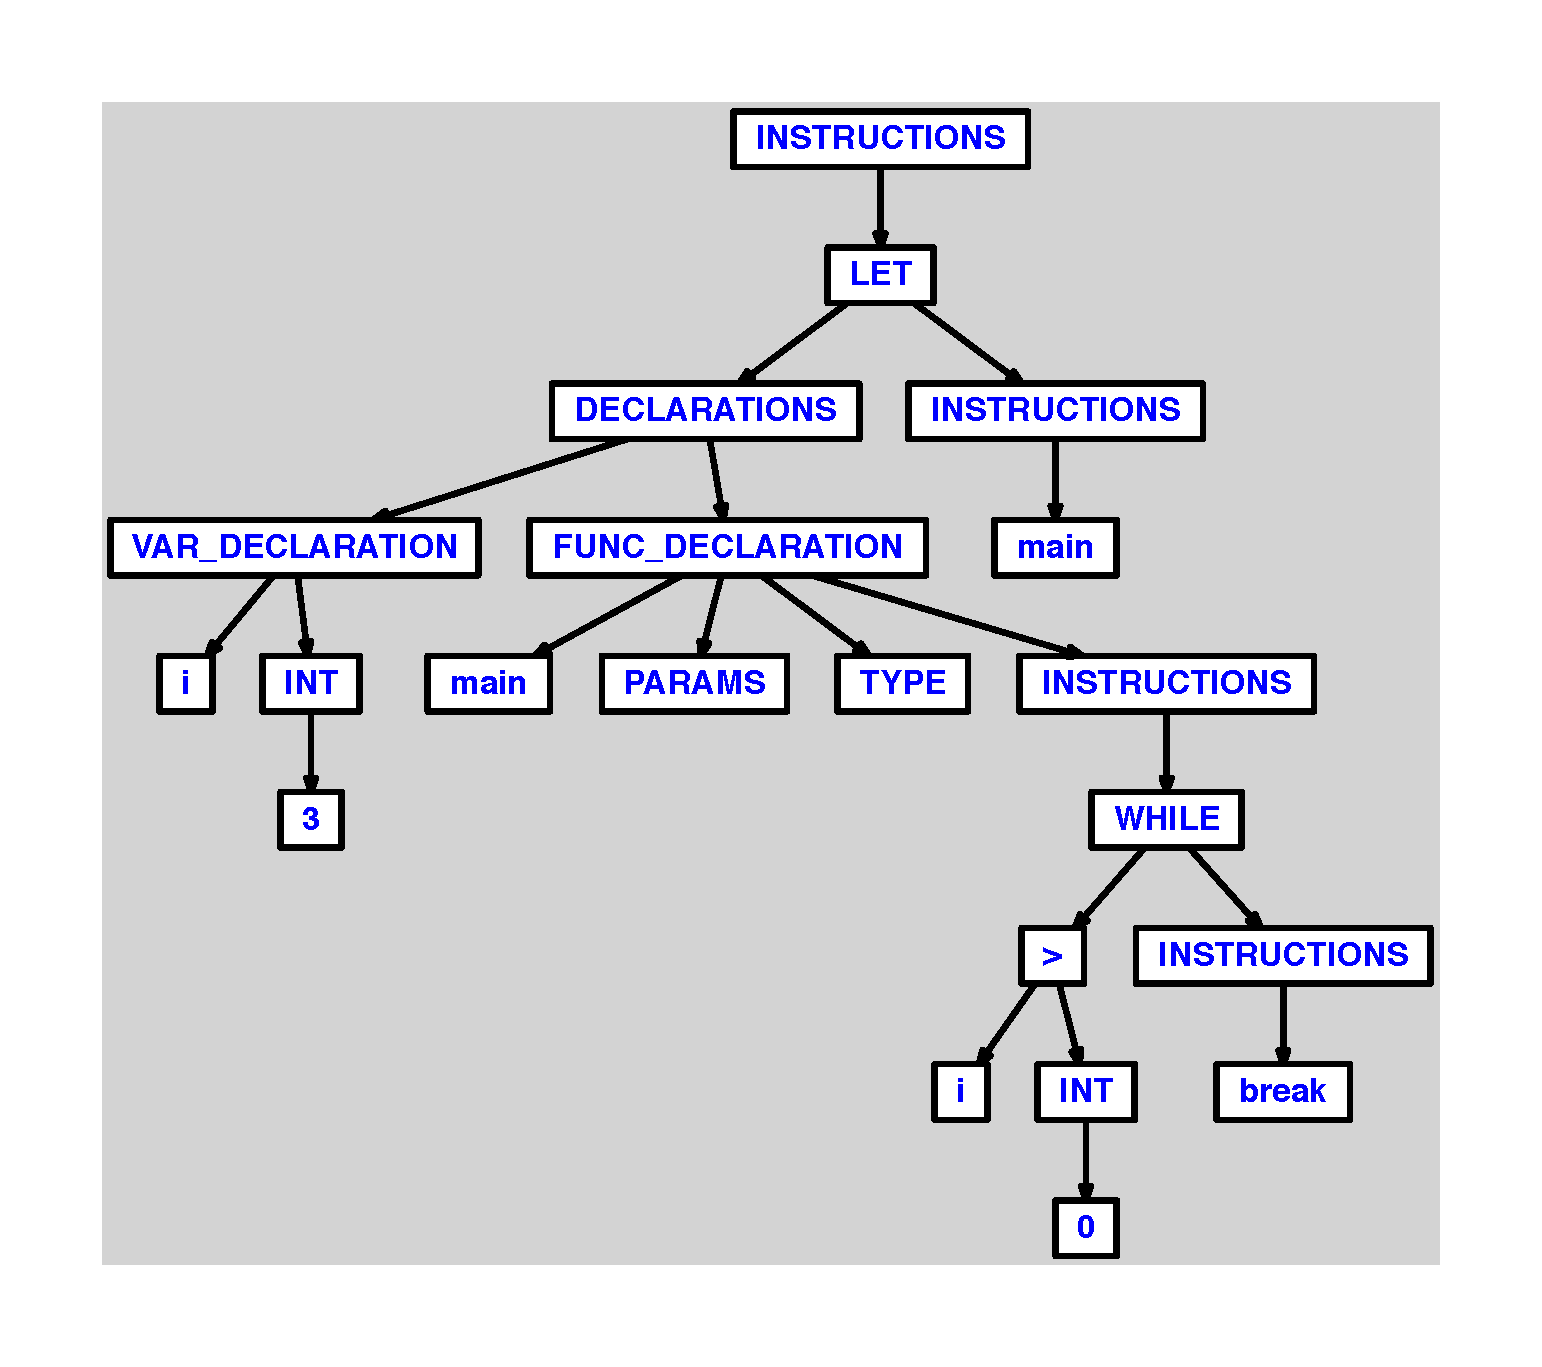
\includegraphics[max width=\textwidth]{ast/ast_15.pdf}\end{figure}\subsubsection{break dans un if then, apres instruction}
\begin{verbatimtab}
let
	var i := 3

	function main() =
		if i=3 then
			print("test");
			break
in main() end
\end{verbatimtab}
\begin{figure}[H]\centering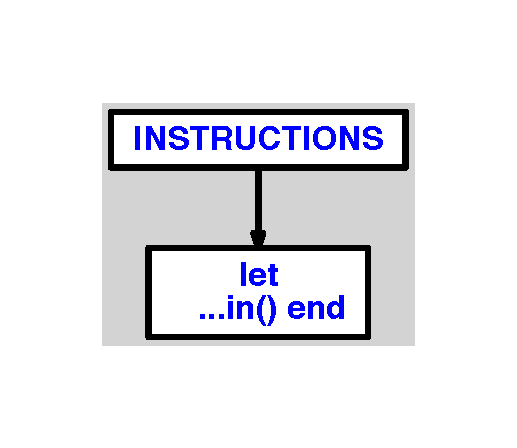
\includegraphics[max width=\textwidth]{ast/ast_16.pdf}\end{figure}\subsubsection{break dans un if then, sans instruction avant}
\begin{verbatimtab}
let
	var i := 3

	function main() =
		if i=3 then
			break
in main() end
\end{verbatimtab}
\begin{figure}[H]\centering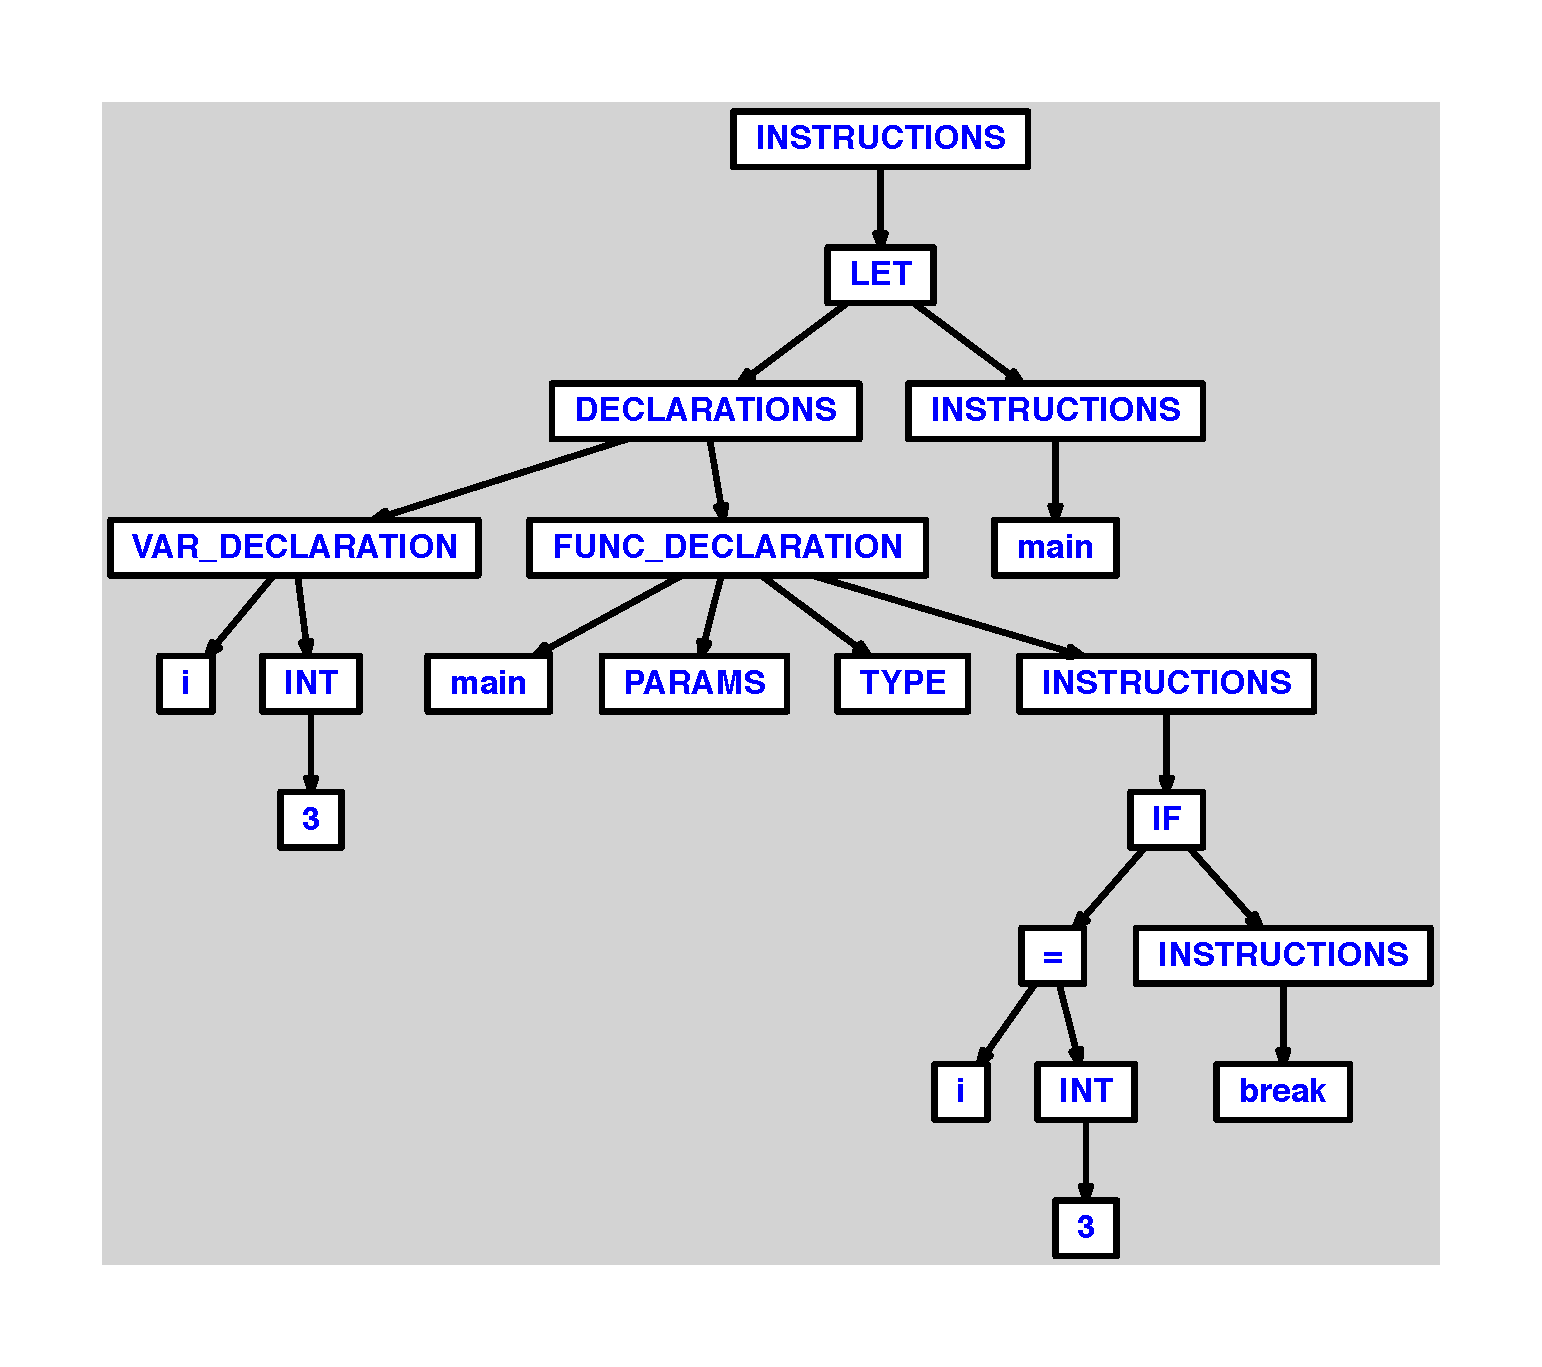
\includegraphics[max width=\textwidth]{ast/ast_17.pdf}\end{figure}\subsubsection{break dans un if then else, apres instruction}
\begin{verbatimtab}
let
	var i := 3

	function main() =
		if i=3 then
			i := 2
		else
			print("test");
			break
in main() end
\end{verbatimtab}
\begin{figure}[H]\centering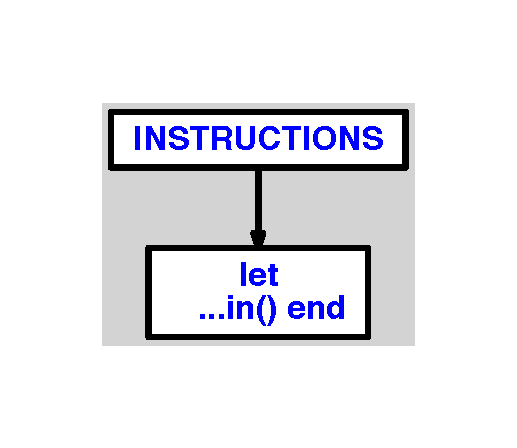
\includegraphics[max width=\textwidth]{ast/ast_18.pdf}\end{figure}\subsubsection{break dans un if then else, sans instruction avant}
\begin{verbatimtab}
let
	var i := 3

	function main() =
		if i=3 then
			i := 2
		else
			break
in main() end
\end{verbatimtab}
\begin{figure}[H]\centering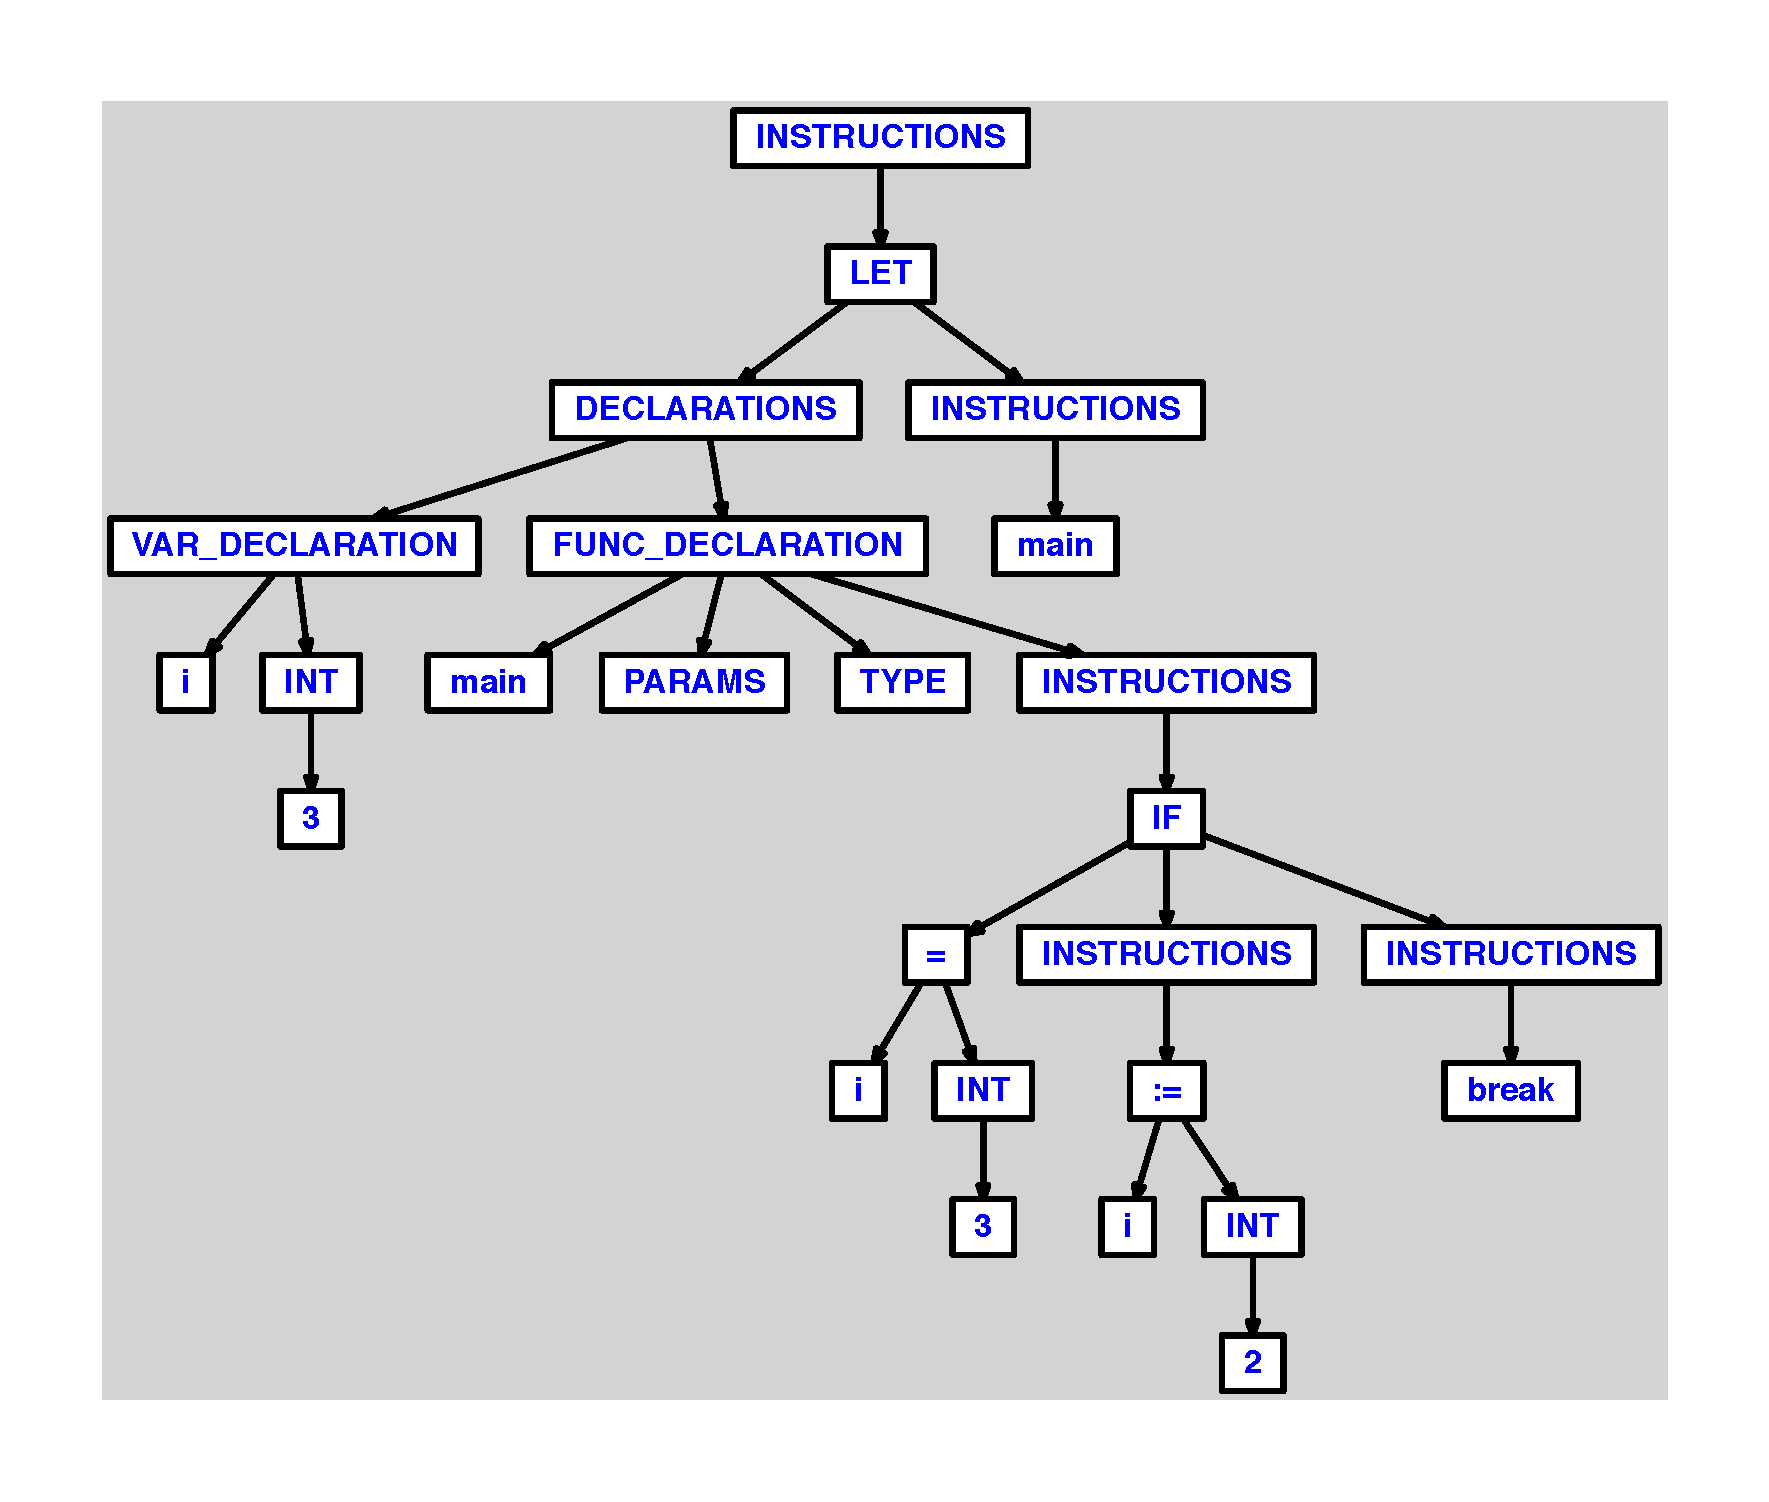
\includegraphics[max width=\textwidth]{ast/ast_19.pdf}\end{figure}\subsubsection{break seul}
\begin{verbatimtab}
break
\end{verbatimtab}
\begin{figure}[H]\centering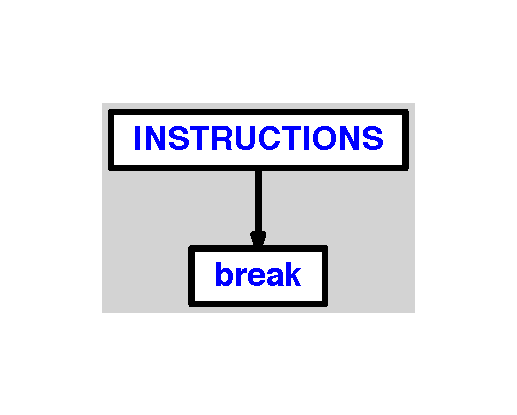
\includegraphics[max width=\textwidth]{ast/ast_20.pdf}\end{figure}\subsubsection{break seul, apres saut de ligne}
\begin{verbatimtab}

break
\end{verbatimtab}
\begin{figure}[H]\centering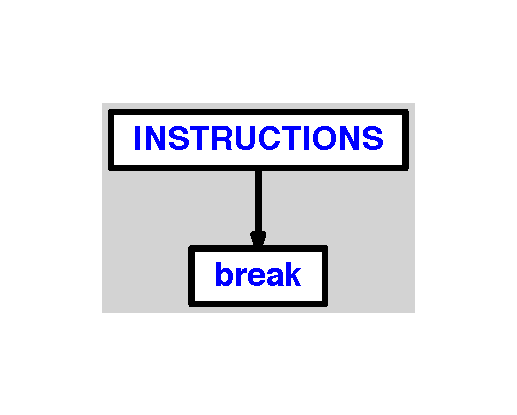
\includegraphics[max width=\textwidth]{ast/ast_21.pdf}\end{figure}\section{calculation}
\subsection{KO}
\subsubsection{addition avec operateur mal ecrit}
\begin{verbatimtab}
let
	function main() = printi(1++2)
in main() end
\end{verbatimtab}
\begin{figure}[H]\centering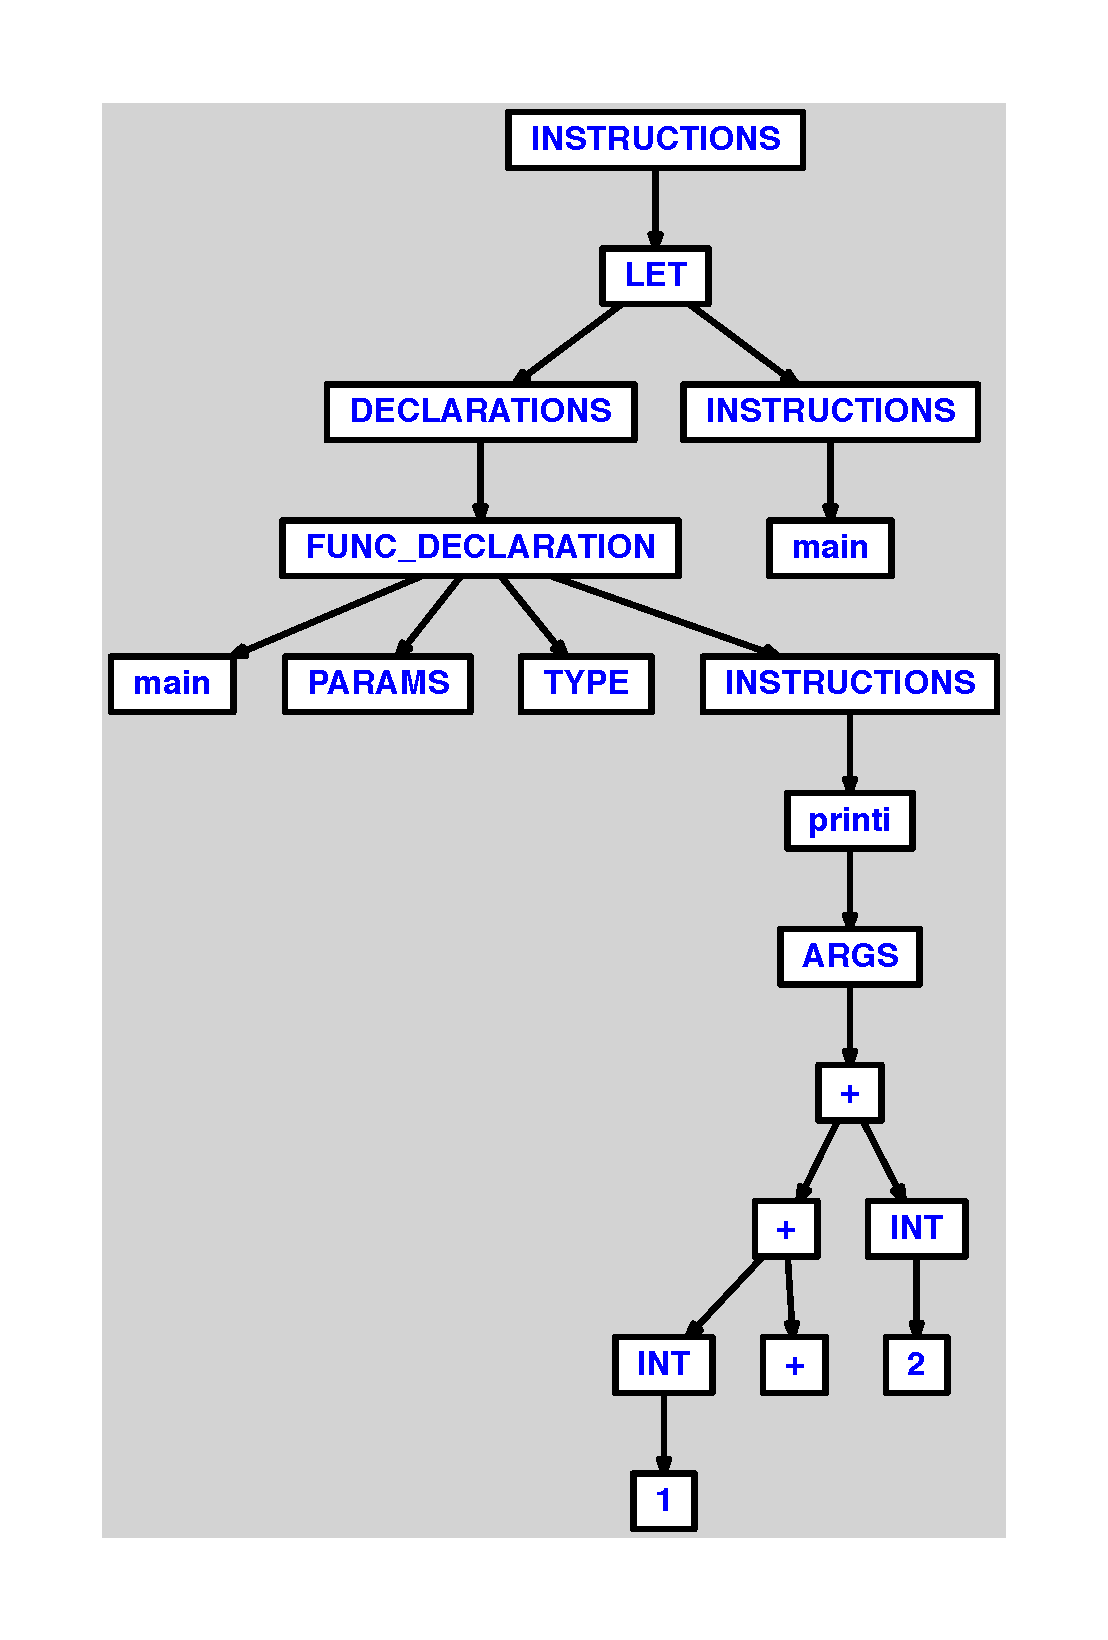
\includegraphics[max width=\textwidth]{ast/ast_22.pdf}\end{figure}\subsubsection{soustraction avec operateur mal ecrit}
\begin{verbatimtab}
let
	function main() = printi(2--1)
in main() end
\end{verbatimtab}
\begin{figure}[H]\centering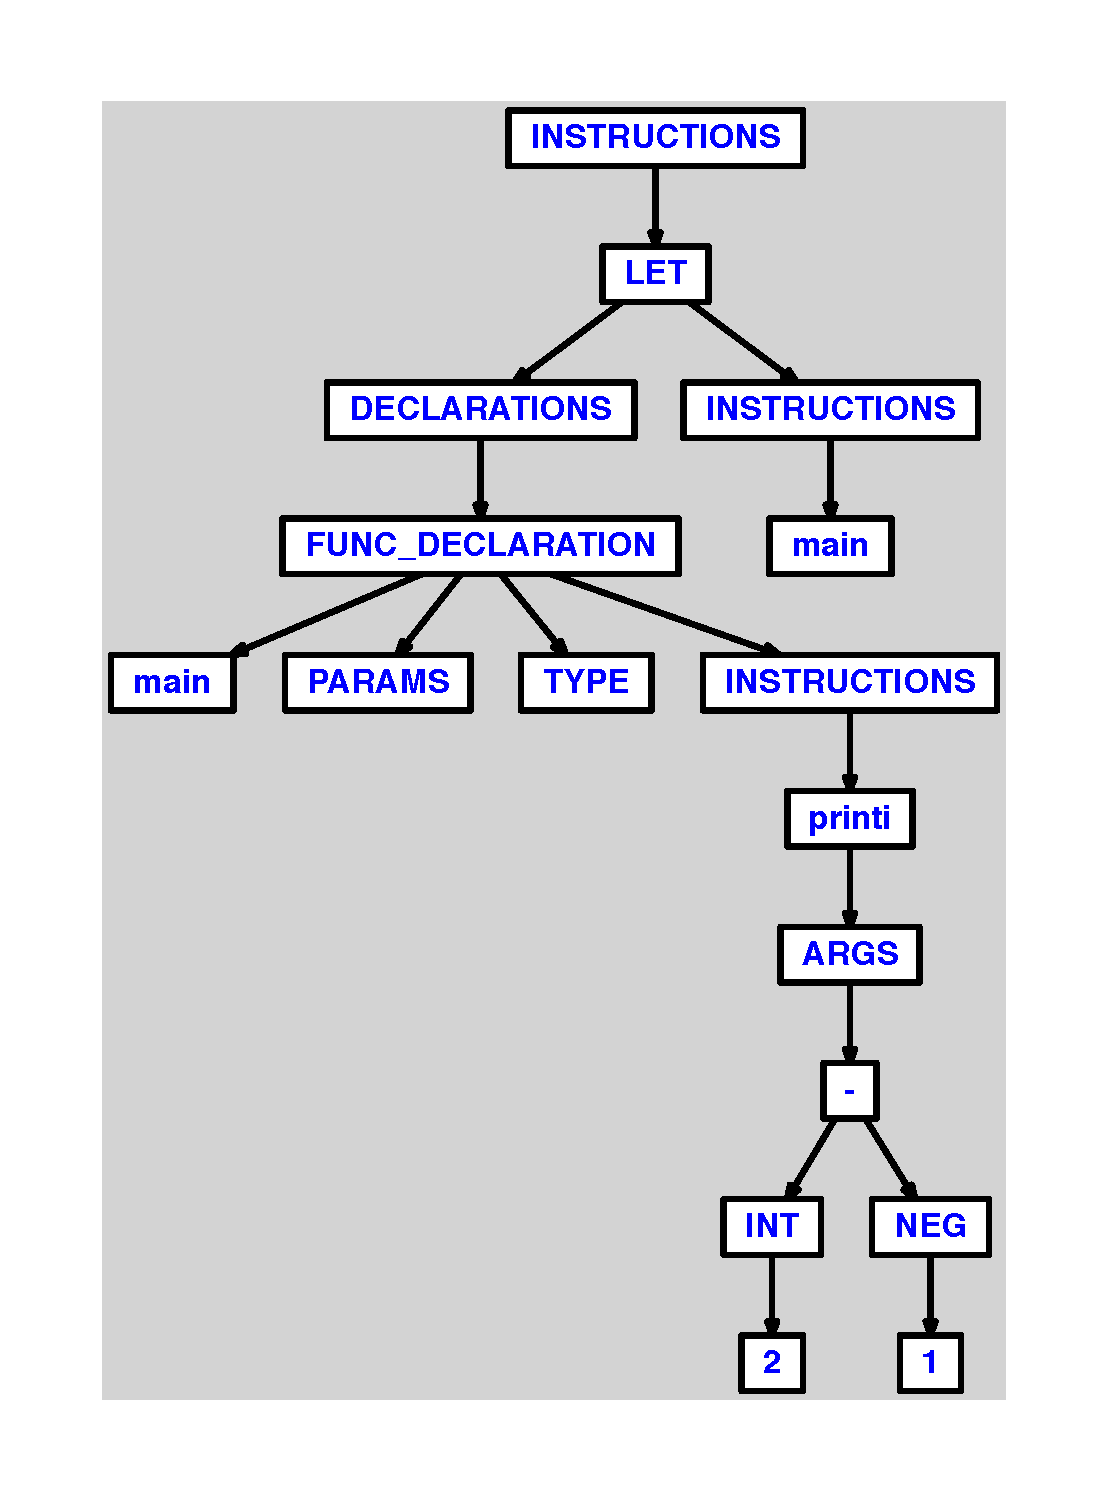
\includegraphics[max width=\textwidth]{ast/ast_23.pdf}\end{figure}\subsubsection{multiplication avec operateur mal ecrit}
\begin{verbatimtab}
let
	function main() = printi(1**2)
in main() end
\end{verbatimtab}
\begin{figure}[H]\centering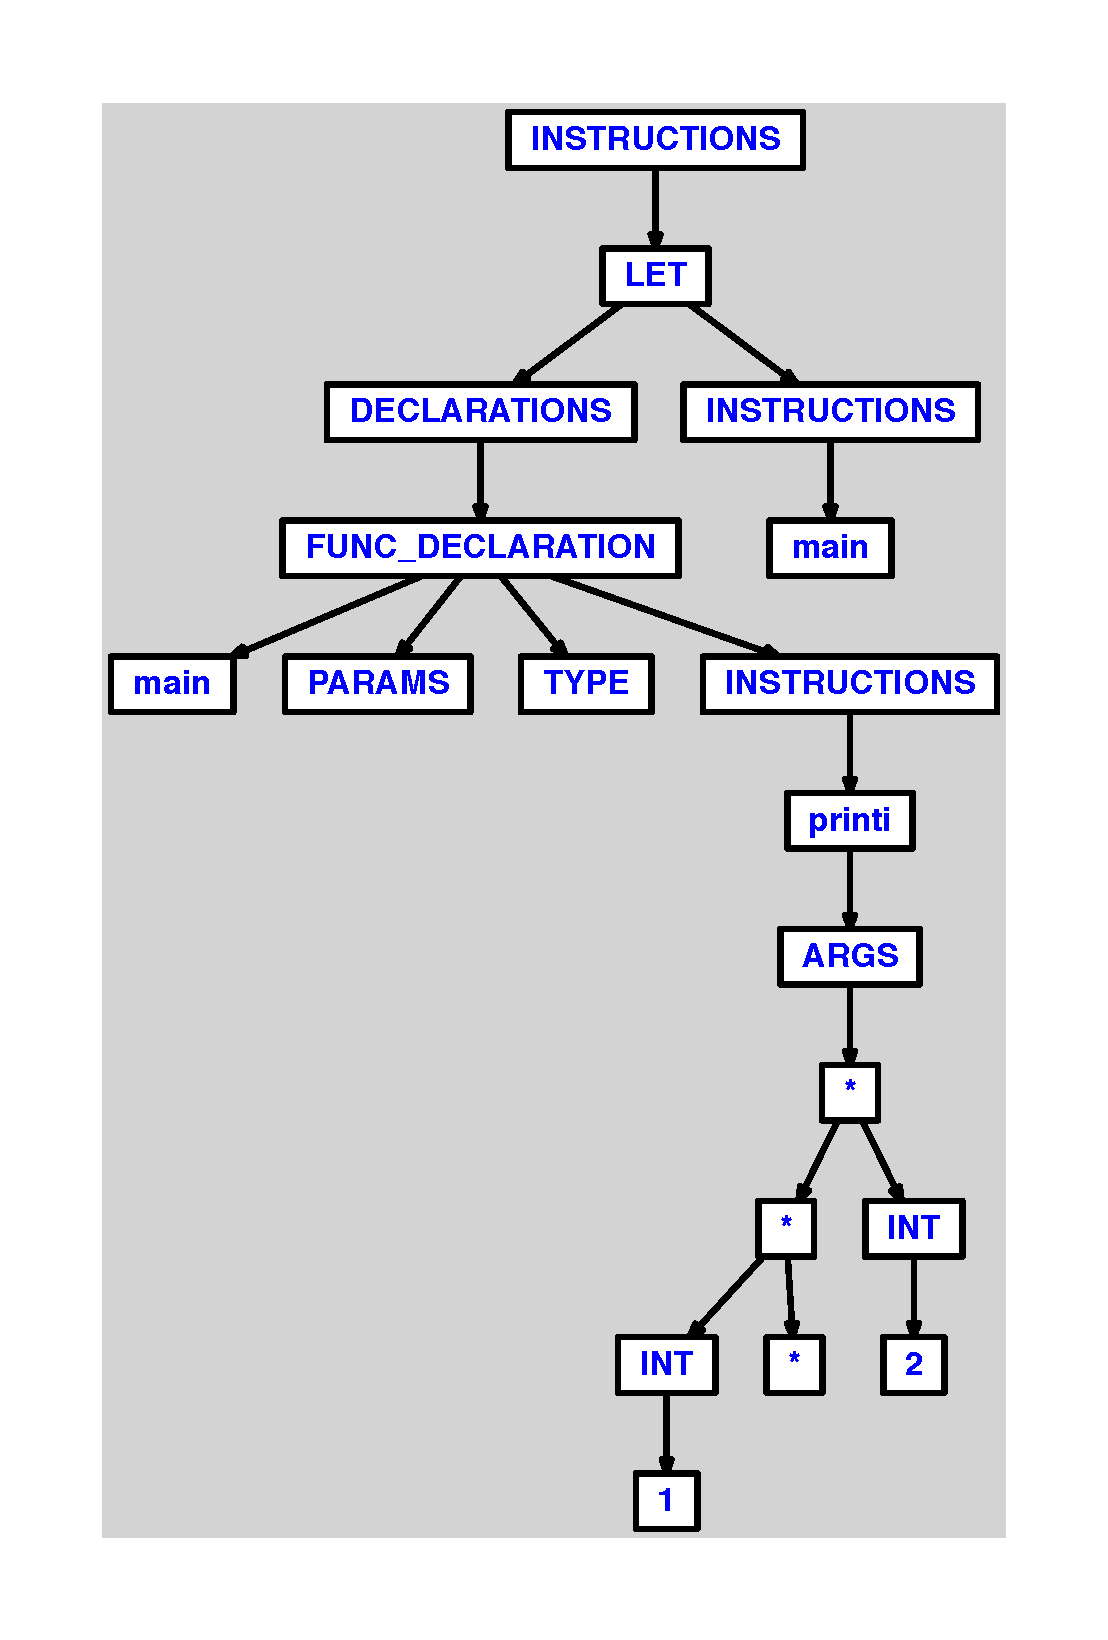
\includegraphics[max width=\textwidth]{ast/ast_24.pdf}\end{figure}\subsubsection{division avec operateur mal ecrit}
\begin{verbatimtab}
let
	function main() = printi(2//1)
in main() end
\end{verbatimtab}
\begin{figure}[H]\centering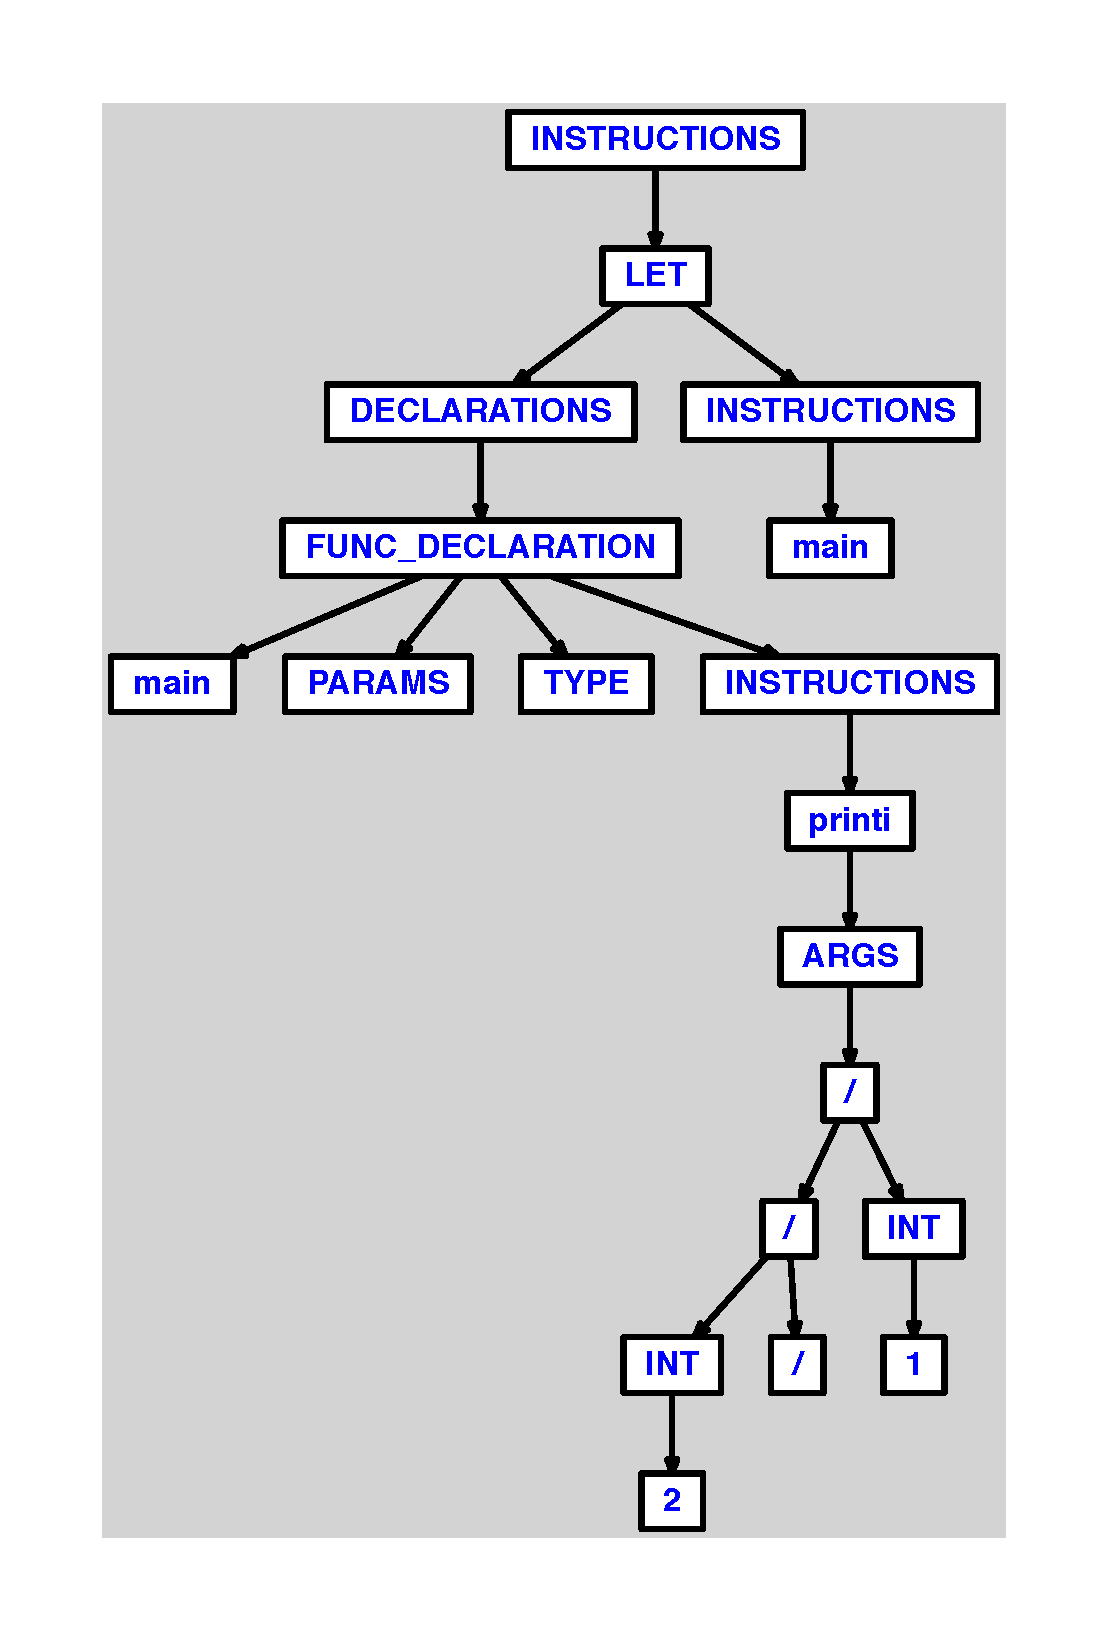
\includegraphics[max width=\textwidth]{ast/ast_25.pdf}\end{figure}\subsubsection{moins unaire avec operateur mal ecrit}
\begin{verbatimtab}
let
	function main() = printi(--1)
in main() end
\end{verbatimtab}
\begin{figure}[H]\centering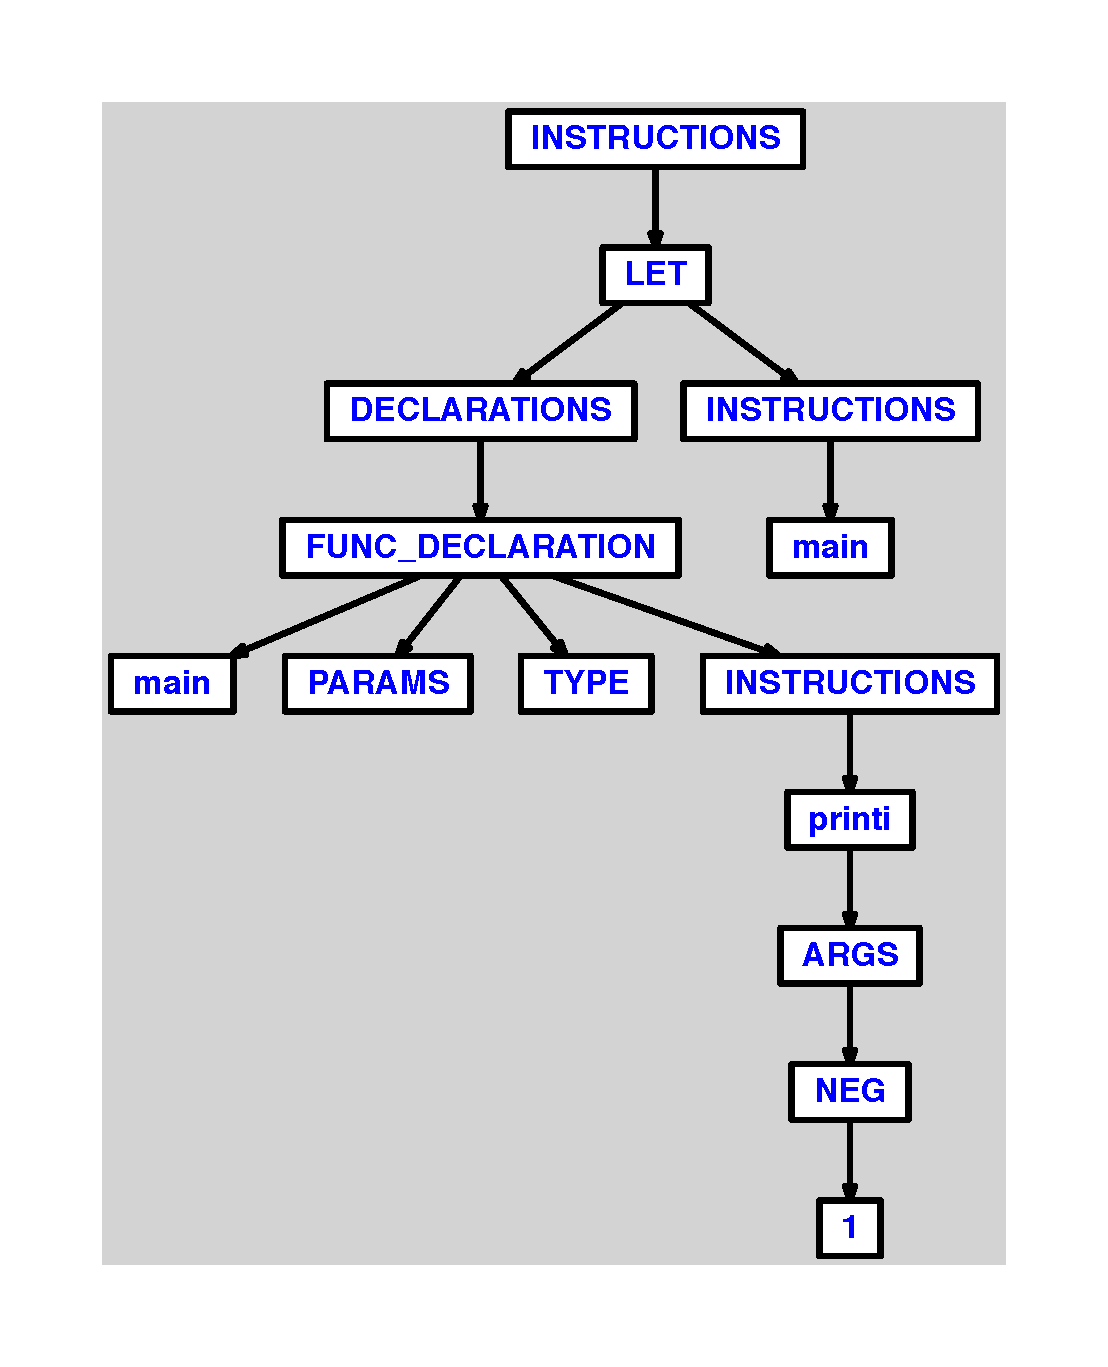
\includegraphics[max width=\textwidth]{ast/ast_26.pdf}\end{figure}\subsubsection{calcul a 2 termes avec oubli de parenthese gauche}
\begin{verbatimtab}
let function main() = printi(1+2)) in main() end
\end{verbatimtab}
\begin{figure}[H]\centering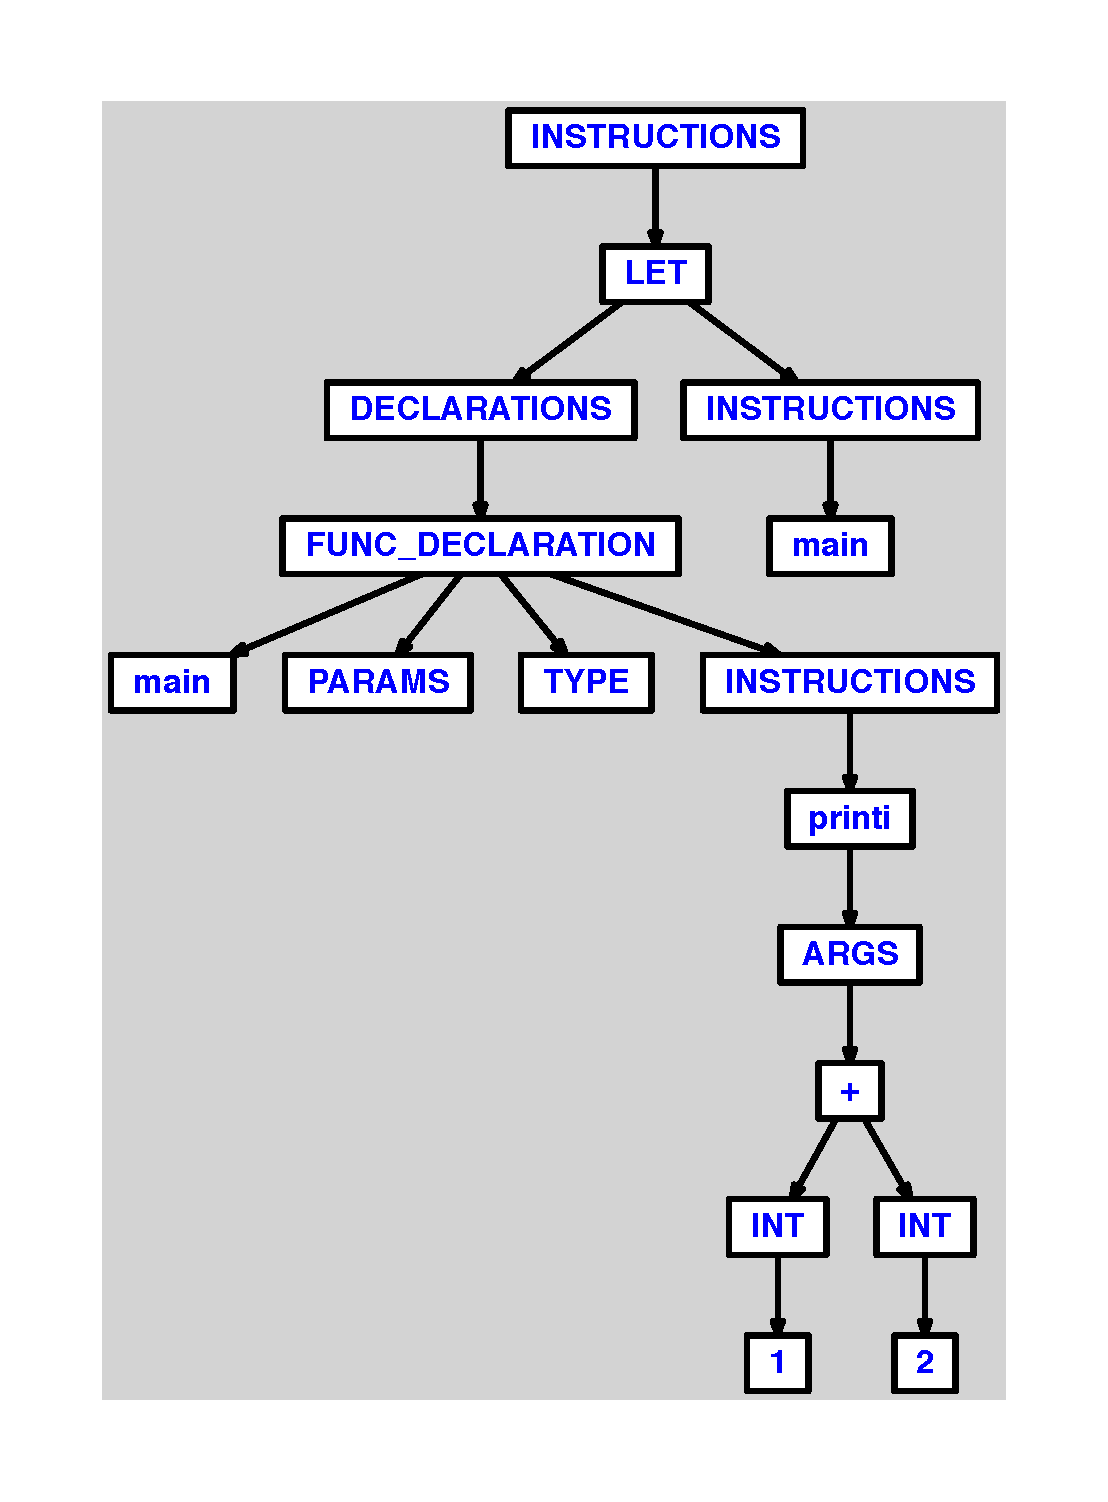
\includegraphics[max width=\textwidth]{ast/ast_27.pdf}\end{figure}\subsubsection{calcul a 2 termes avec oubli de parenthese droite}
\begin{verbatimtab}
let function main() = printi((1+2) in main() end
\end{verbatimtab}
\begin{figure}[H]\centering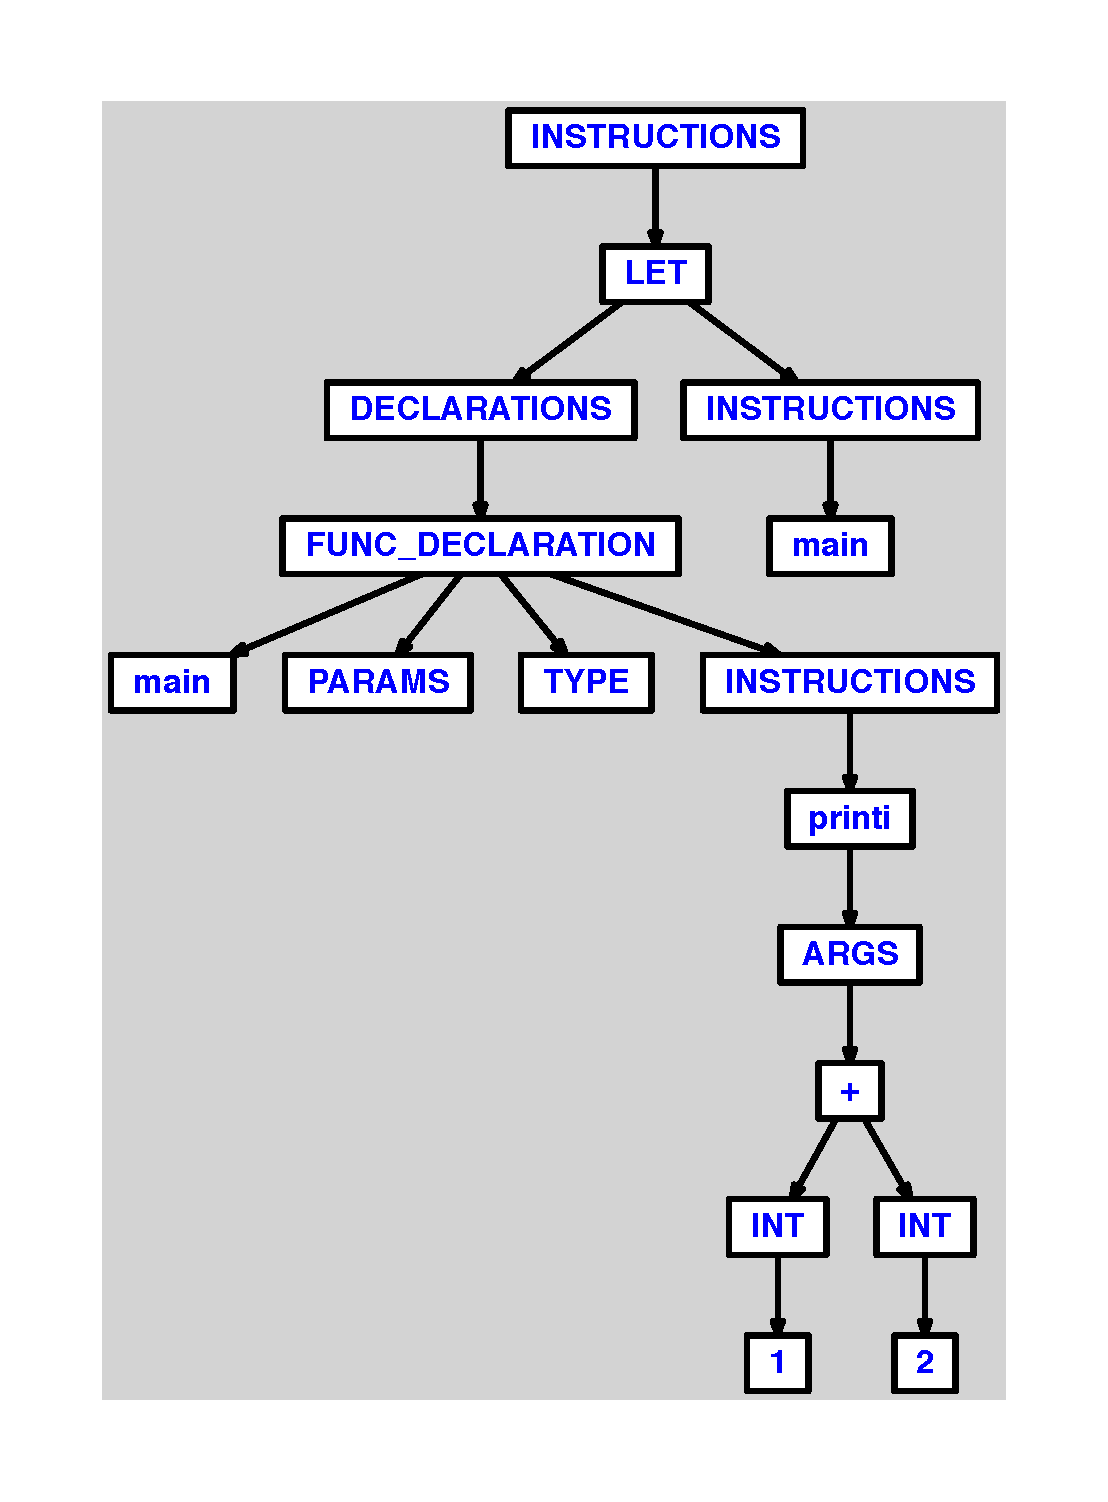
\includegraphics[max width=\textwidth]{ast/ast_28.pdf}\end{figure}\subsubsection{calcul a 3 termes avec oubli de parenthese gauche}
\begin{verbatimtab}
let function main() = printi(1+(2*3))) in main() end
\end{verbatimtab}
\begin{figure}[H]\centering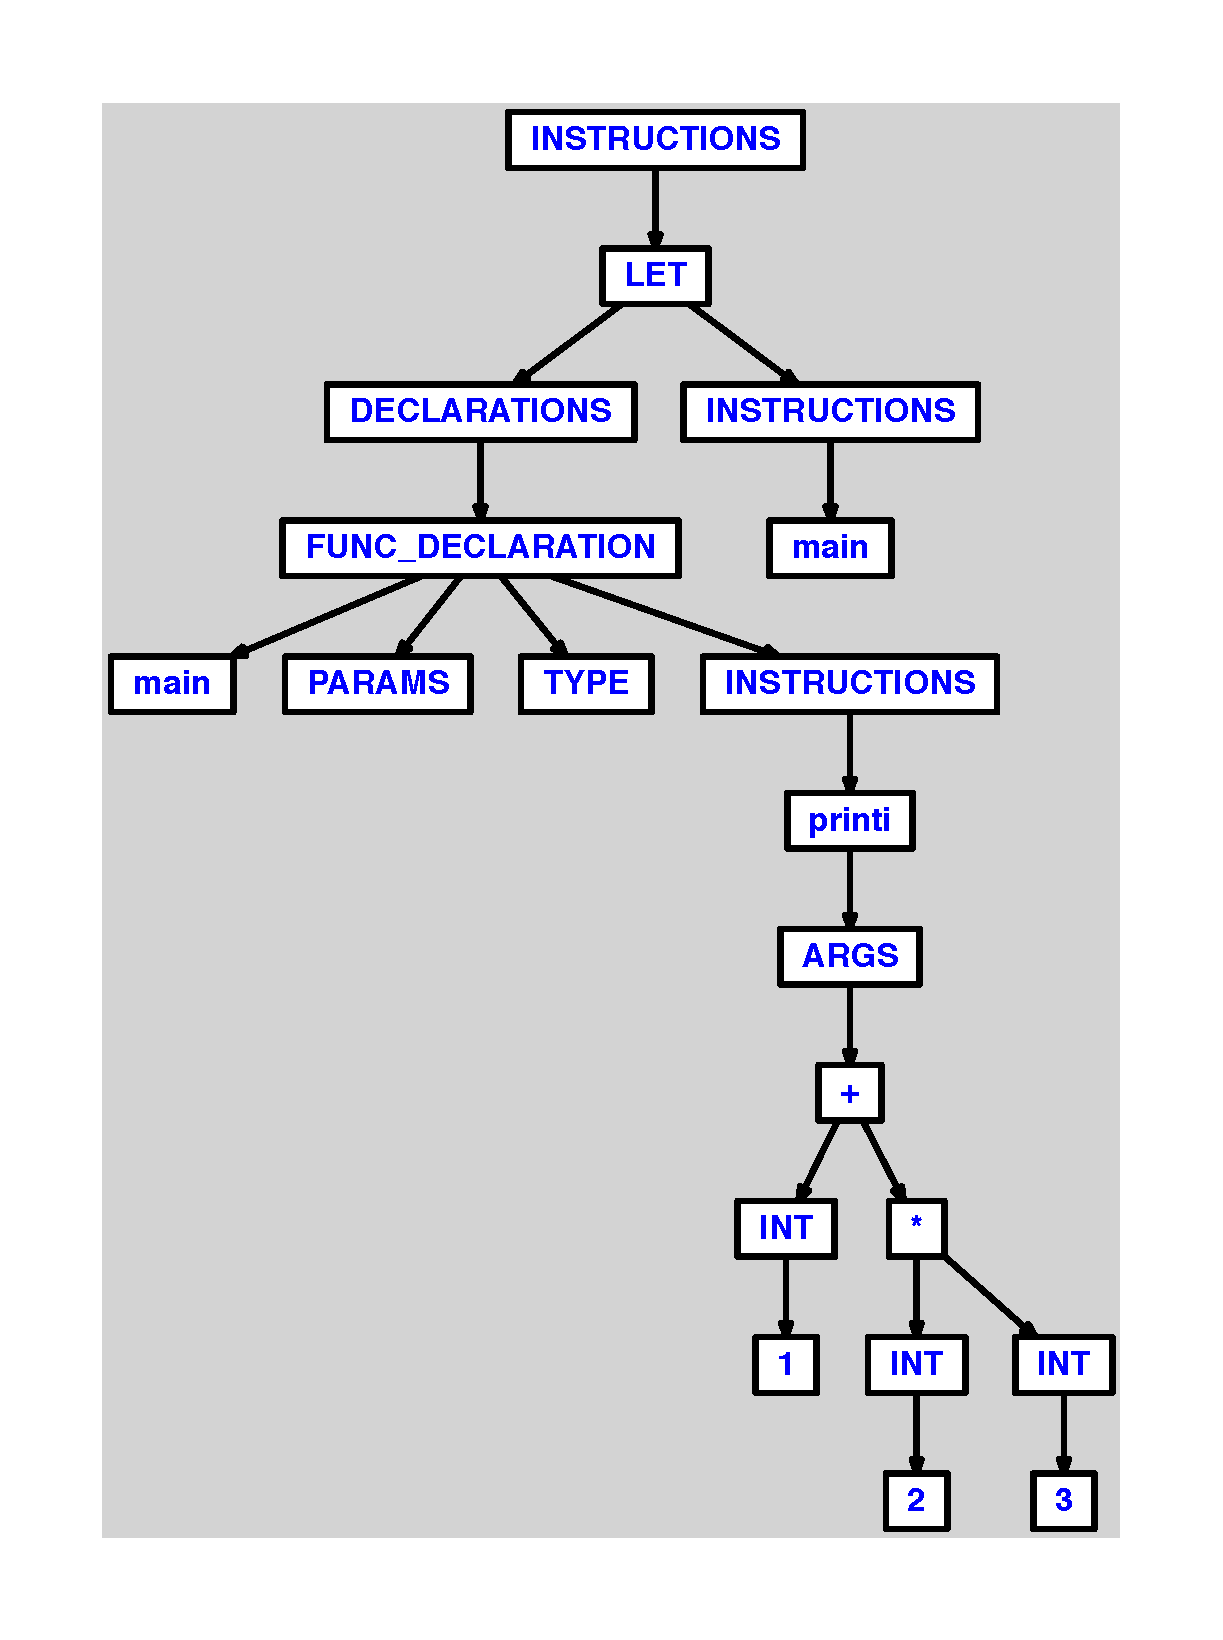
\includegraphics[max width=\textwidth]{ast/ast_29.pdf}\end{figure}\subsubsection{calcul a 3 termes avec oubli de parenthese droite}
\begin{verbatimtab}
let function main() = printi((1+(2*3)) in main() end
\end{verbatimtab}
\begin{figure}[H]\centering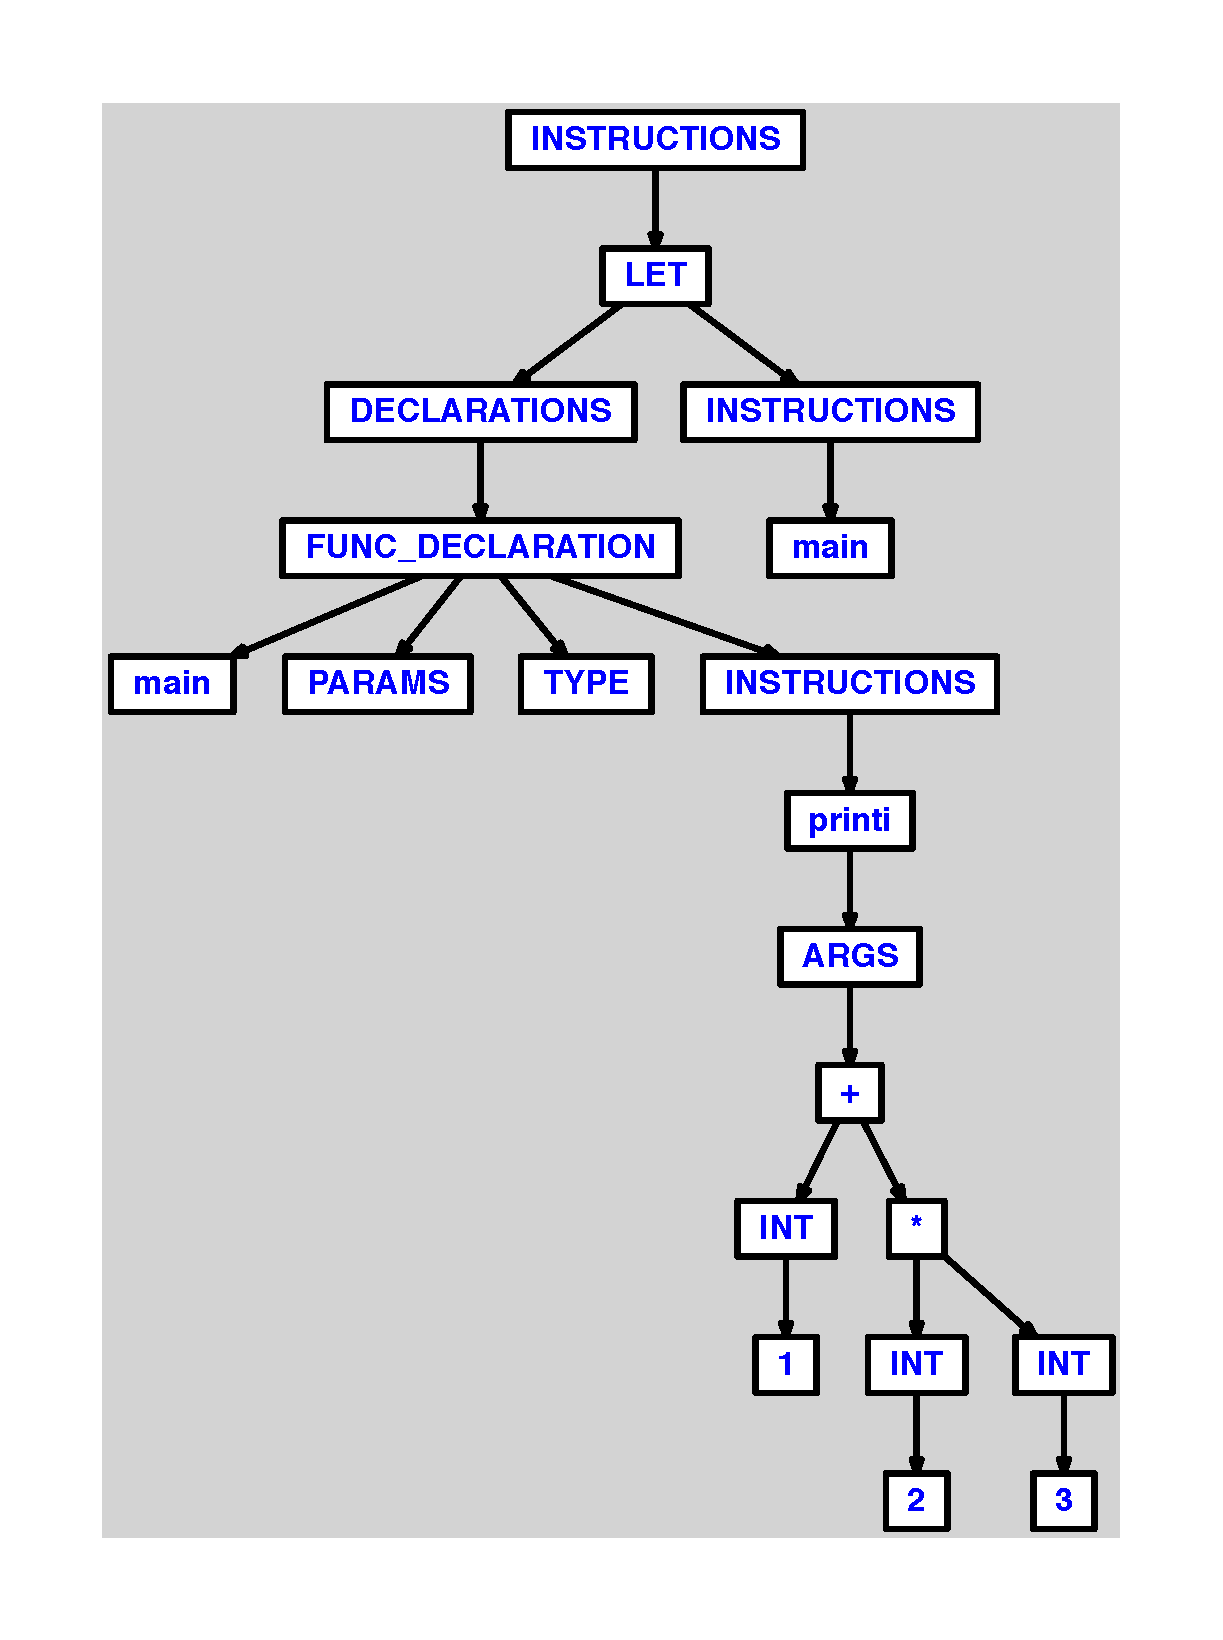
\includegraphics[max width=\textwidth]{ast/ast_30.pdf}\end{figure}\subsubsection{calcul a 4 termes avec oubli de parenthese gauche}
\begin{verbatimtab}
let function main() = printi(1+2)*(2+3)) in main() end
\end{verbatimtab}
\begin{figure}[H]\centering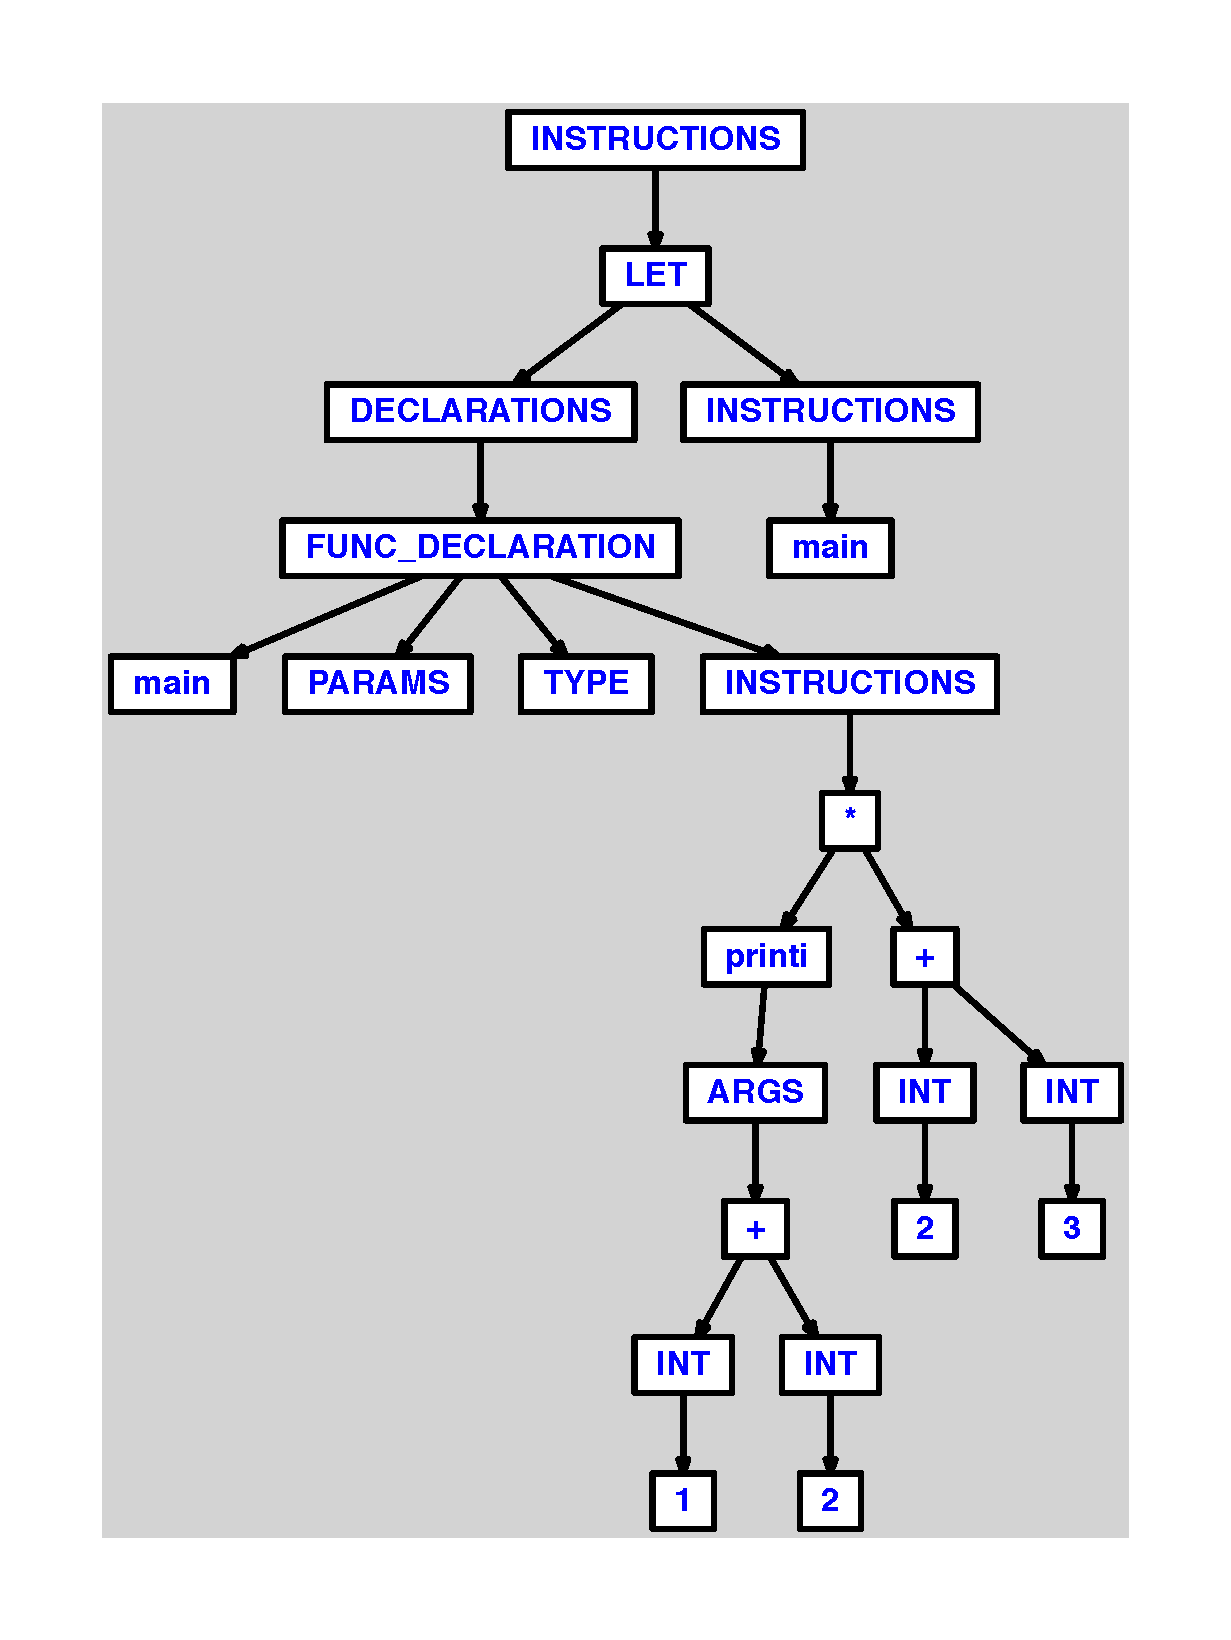
\includegraphics[max width=\textwidth]{ast/ast_31.pdf}\end{figure}\subsubsection{calcul a 4 termes avec oubli de parenthese droite}
\begin{verbatimtab}
let function main() = printi((2-1)/(3-2) in main() end
\end{verbatimtab}
\begin{figure}[H]\centering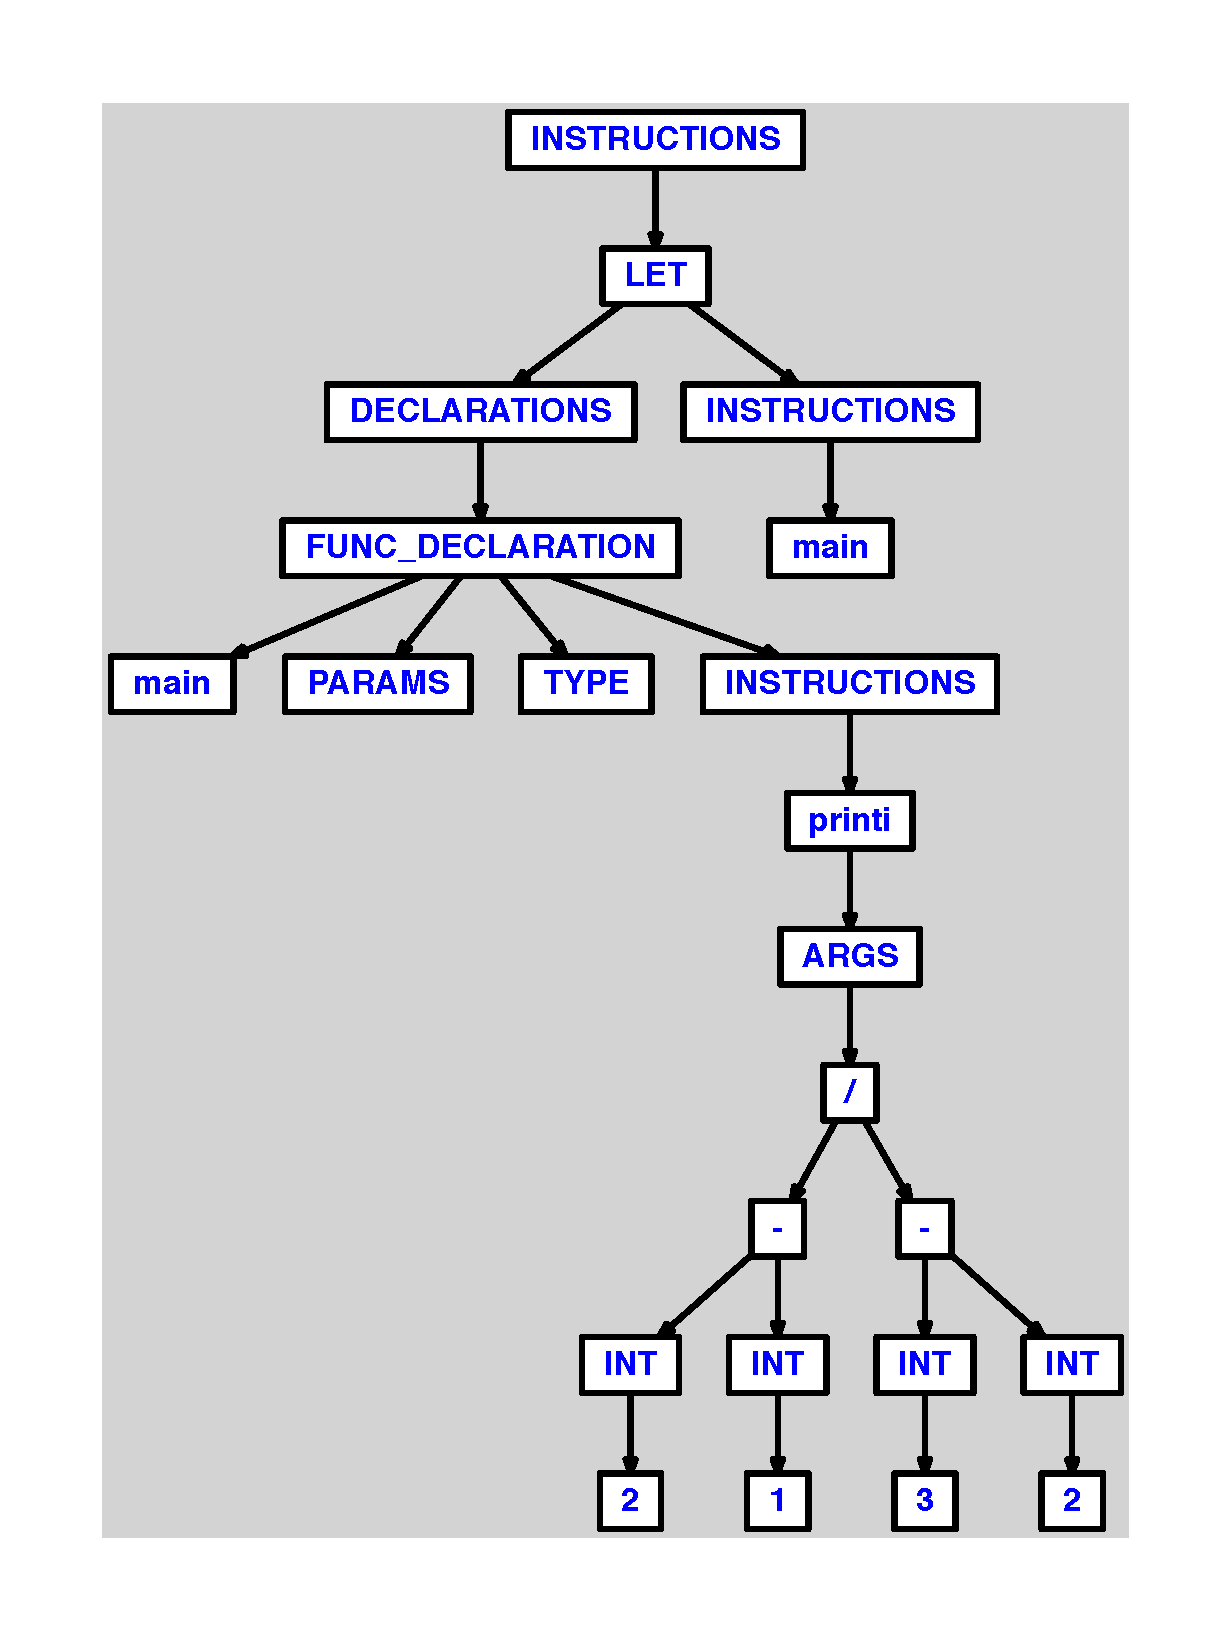
\includegraphics[max width=\textwidth]{ast/ast_32.pdf}\end{figure}\subsubsection{parenthesage sans contenu}
\begin{verbatimtab}
let function main() = () in main() end
\end{verbatimtab}
\begin{figure}[H]\centering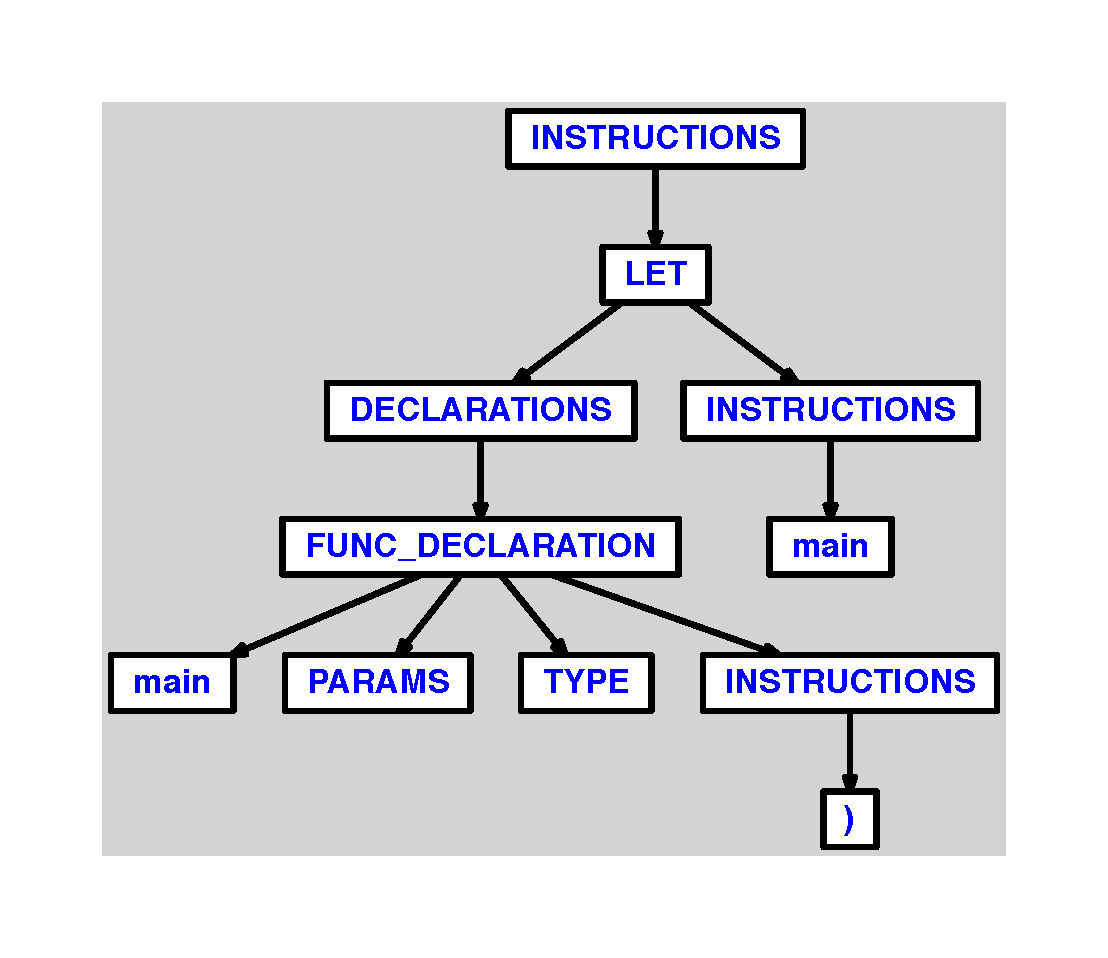
\includegraphics[max width=\textwidth]{ast/ast_33.pdf}\end{figure}\subsubsection{expression parenthesee avec ; en trop}
\begin{verbatimtab}
let function main() = (printi(1);) in main() end
\end{verbatimtab}
\begin{figure}[H]\centering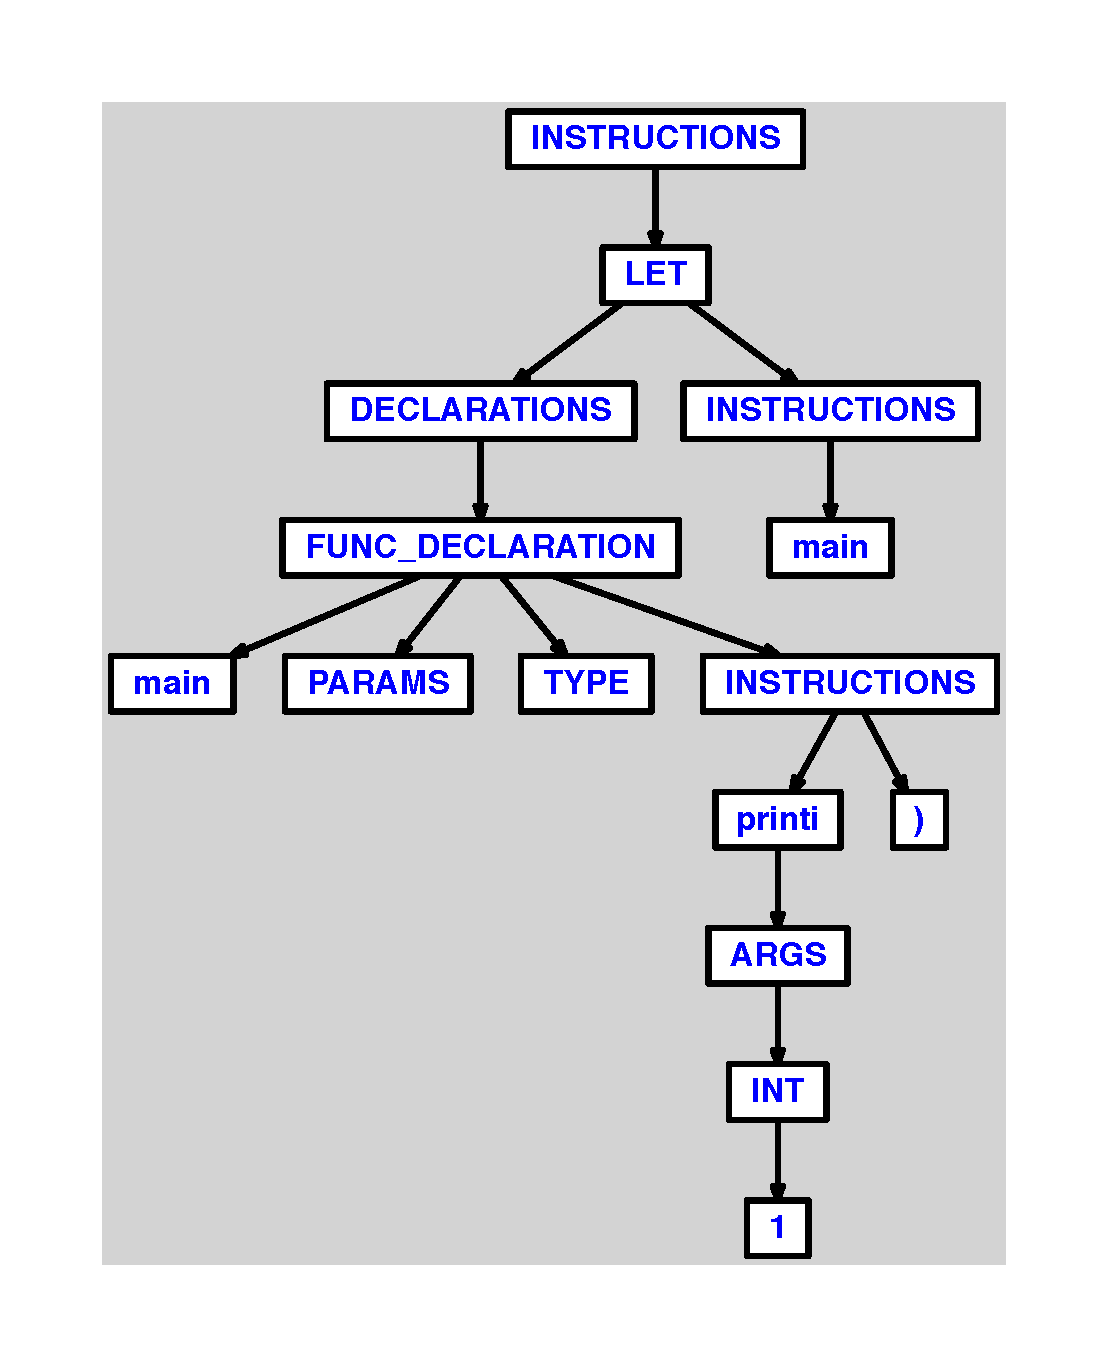
\includegraphics[max width=\textwidth]{ast/ast_34.pdf}\end{figure}\subsubsection{expression parenthesee avec oubli de ;}
\begin{verbatimtab}
let function main() = (printi(1) printi(2)) in main() end
\end{verbatimtab}
\begin{figure}[H]\centering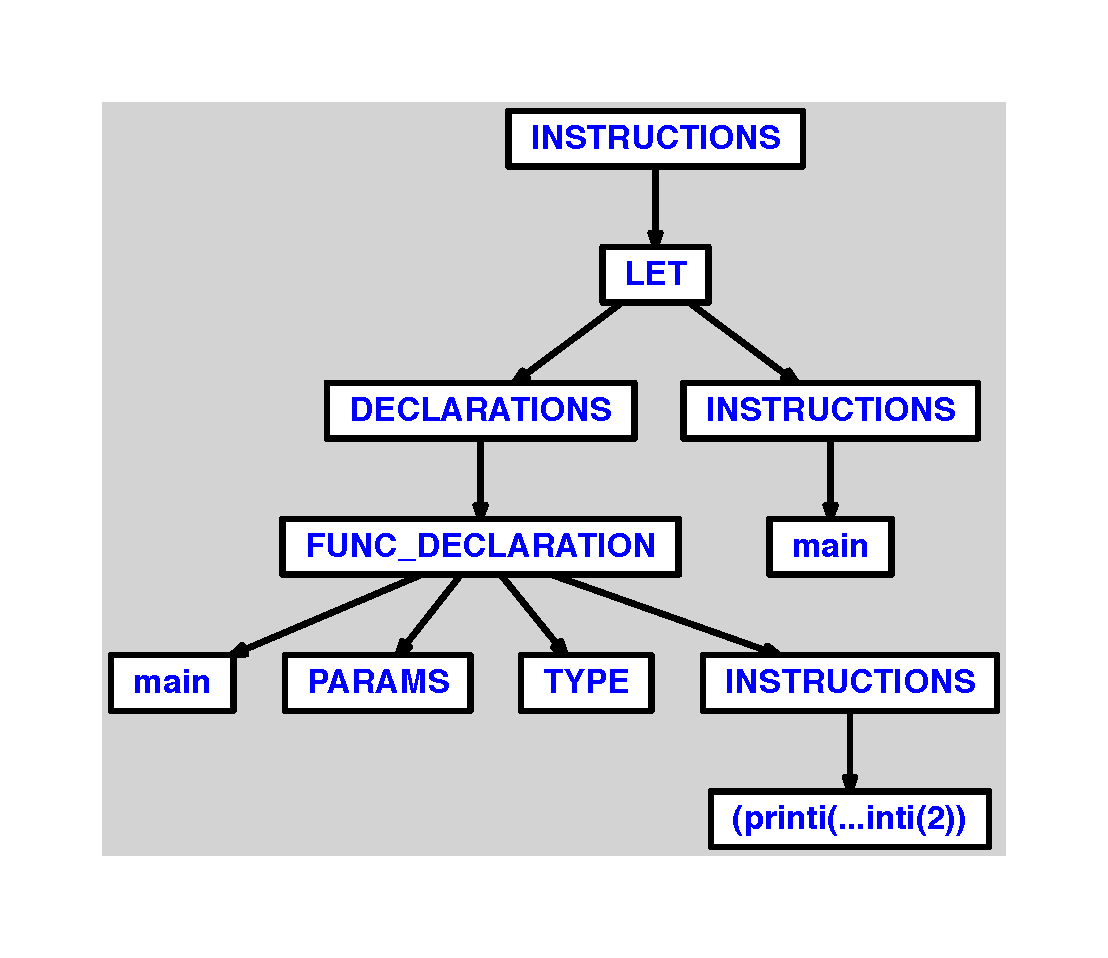
\includegraphics[max width=\textwidth]{ast/ast_35.pdf}\end{figure}\subsubsection{expression non parenthesee avec oubli de ;}
\begin{verbatimtab}
let function main() = printi(1) printi(2) in main() end
\end{verbatimtab}
\begin{figure}[H]\centering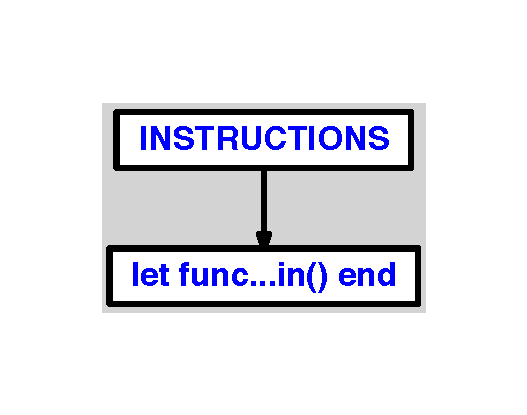
\includegraphics[max width=\textwidth]{ast/ast_36.pdf}\end{figure}\subsubsection{expression non parenthesee avec ; en trop}
\begin{verbatimtab}
let function main() = printi(1); in main() end
\end{verbatimtab}
\begin{figure}[H]\centering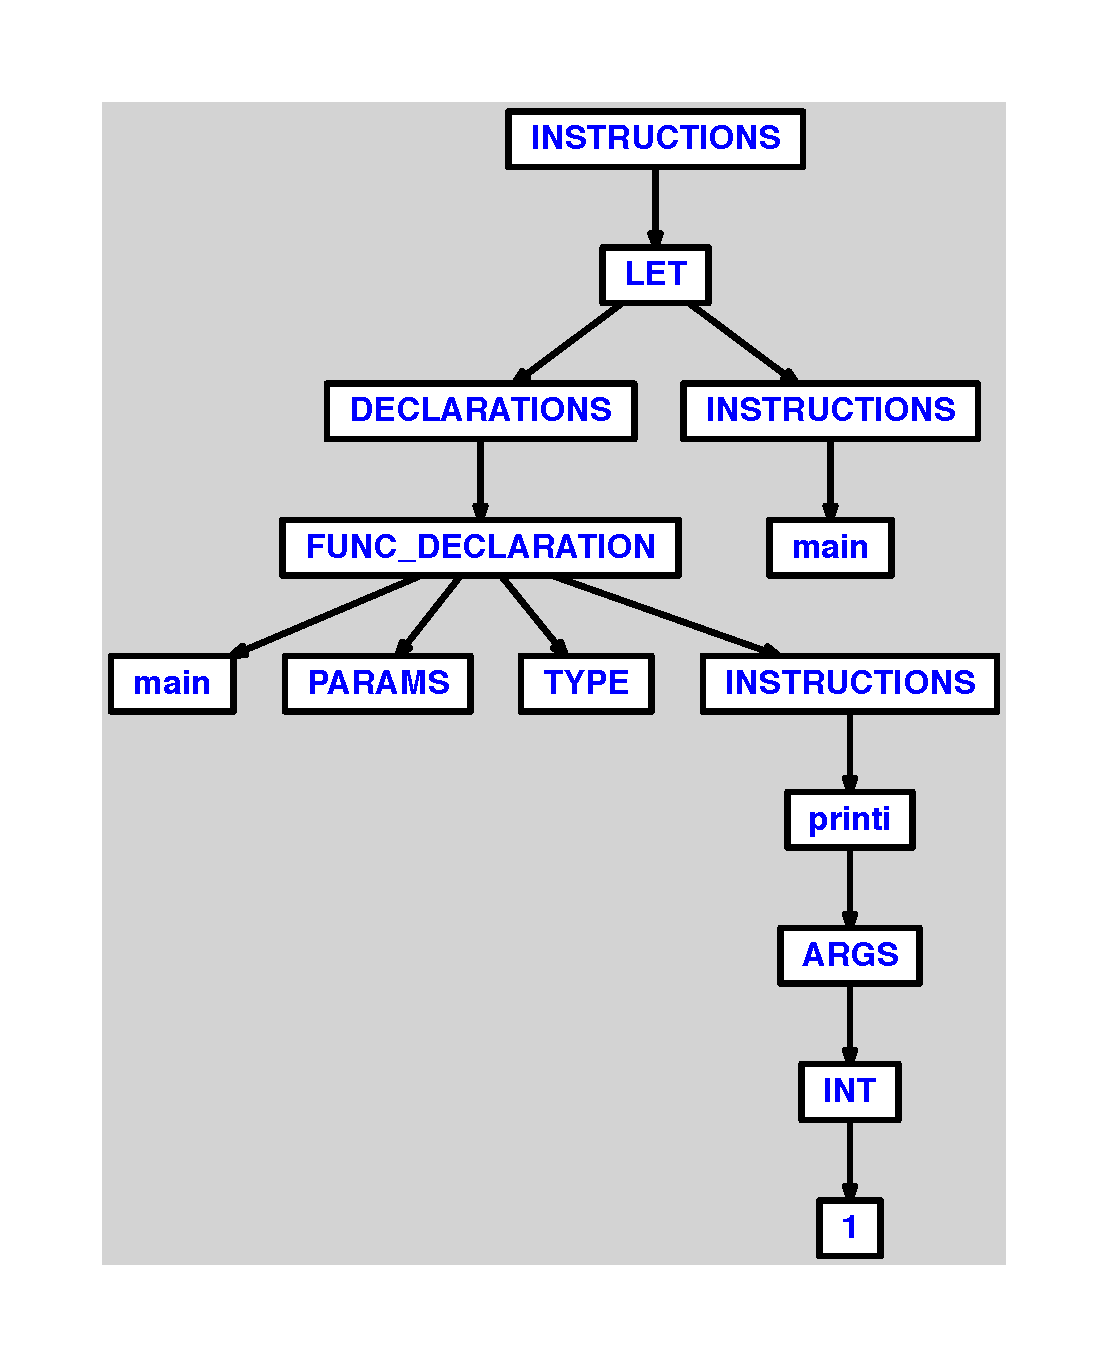
\includegraphics[max width=\textwidth]{ast/ast_37.pdf}\end{figure}\subsubsection{; sans instruction avant}
\begin{verbatimtab}
let function main() = ;
\end{verbatimtab}
\begin{figure}[H]\centering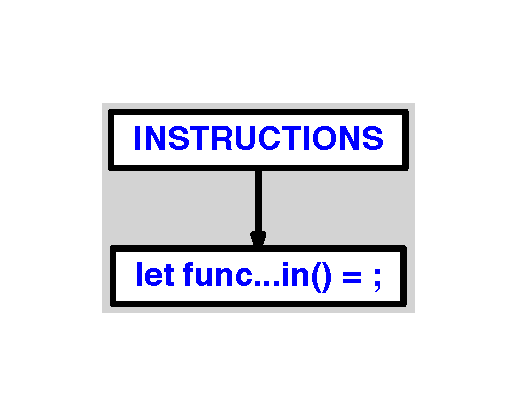
\includegraphics[max width=\textwidth]{ast/ast_38.pdf}\end{figure}\subsection{OK}
\subsubsection{addition simple, a 2 termes}
\begin{verbatimtab}
let
	function main() = printi(1+2)
in main() end
\end{verbatimtab}
\begin{figure}[H]\centering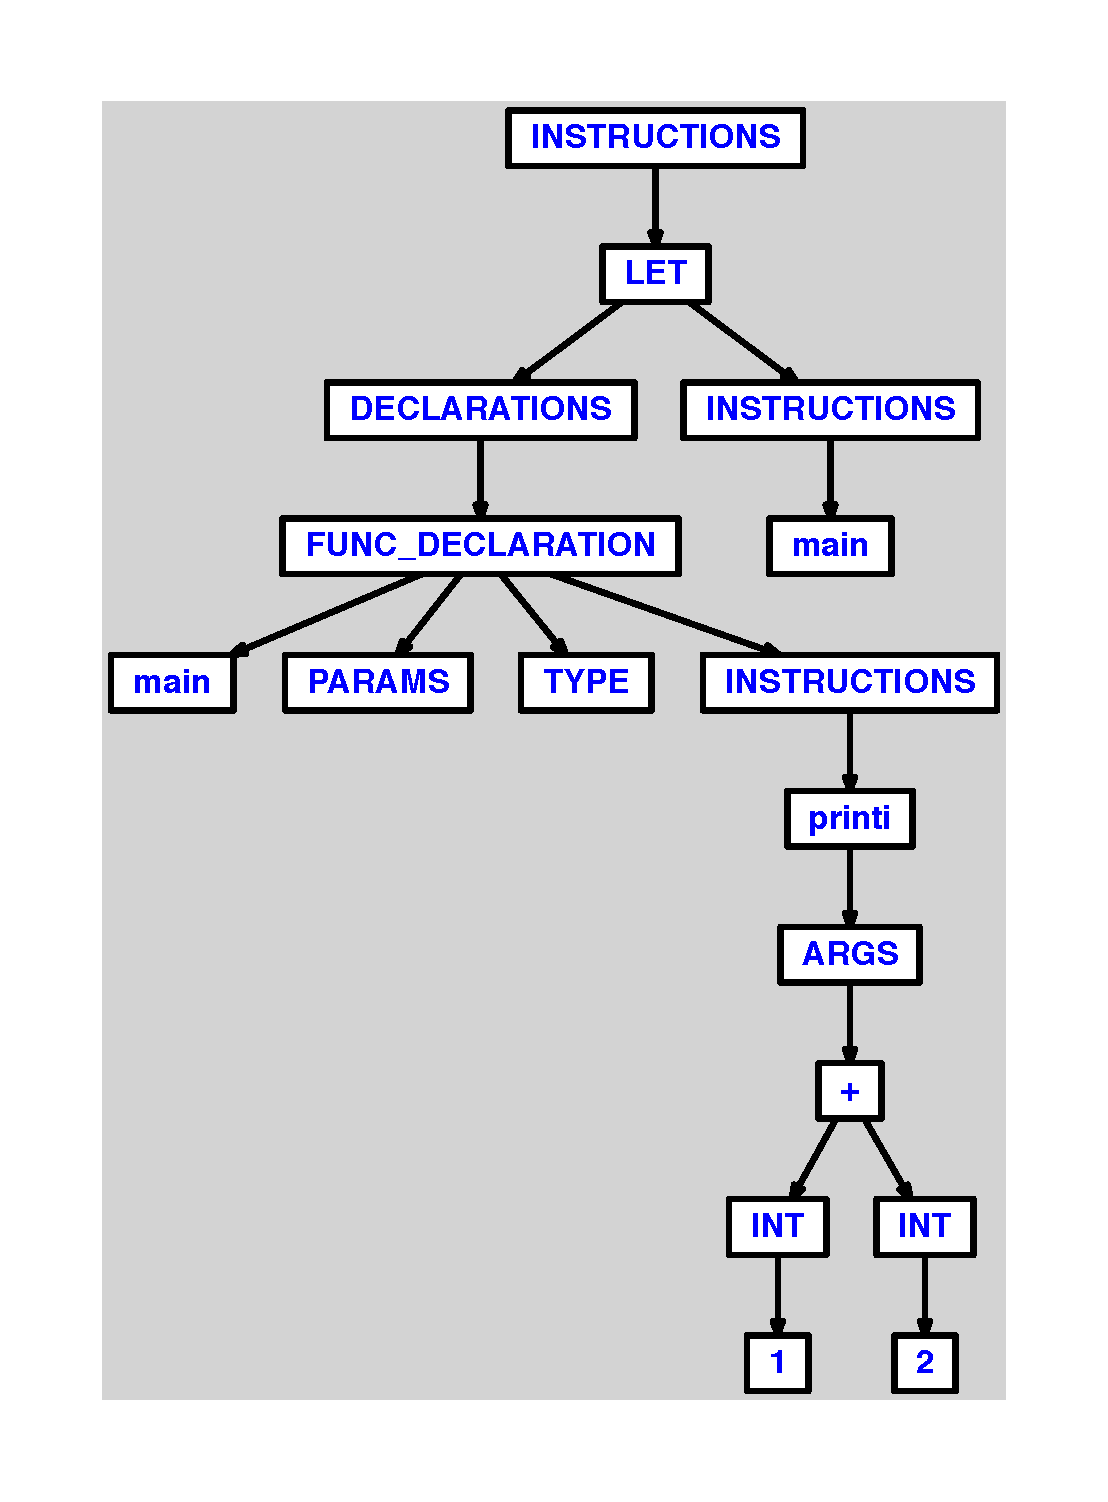
\includegraphics[max width=\textwidth]{ast/ast_39.pdf}\end{figure}\subsubsection{soustraction simple, a 2 termes}
\begin{verbatimtab}
let
	function main() = printi(2-1)
in main() end
\end{verbatimtab}
\begin{figure}[H]\centering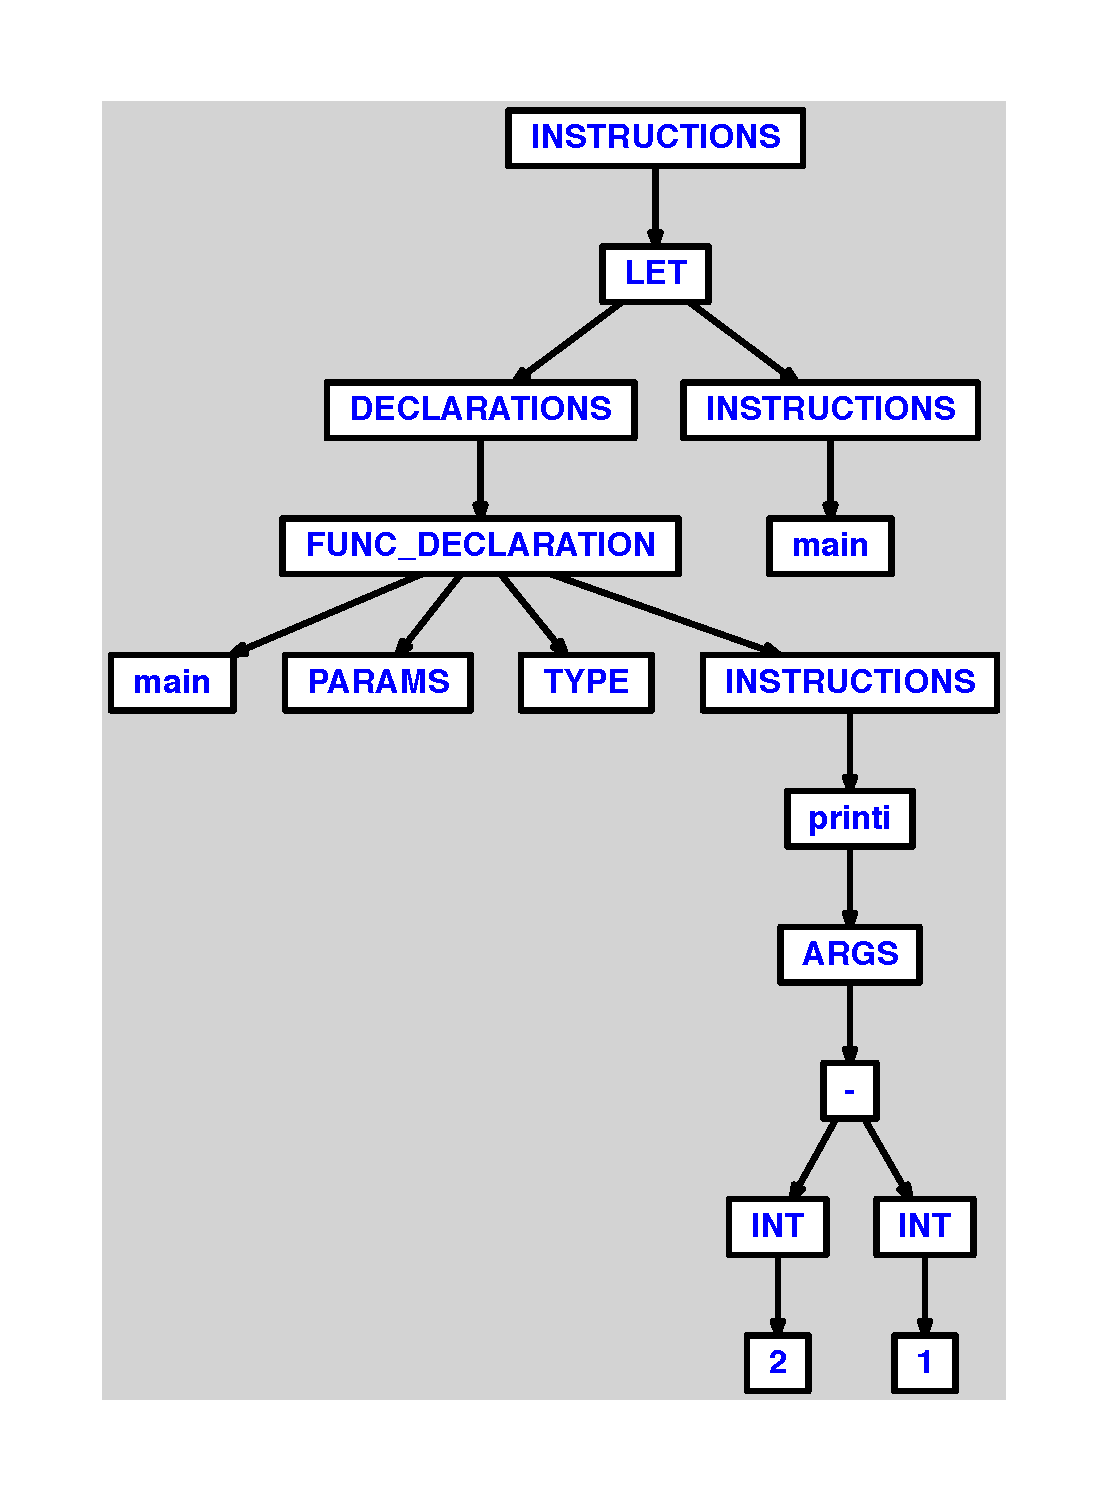
\includegraphics[max width=\textwidth]{ast/ast_40.pdf}\end{figure}\subsubsection{multiplication simple, a 2 termes}
\begin{verbatimtab}
let
	function main() = printi(1*2)
in main() end
\end{verbatimtab}
\begin{figure}[H]\centering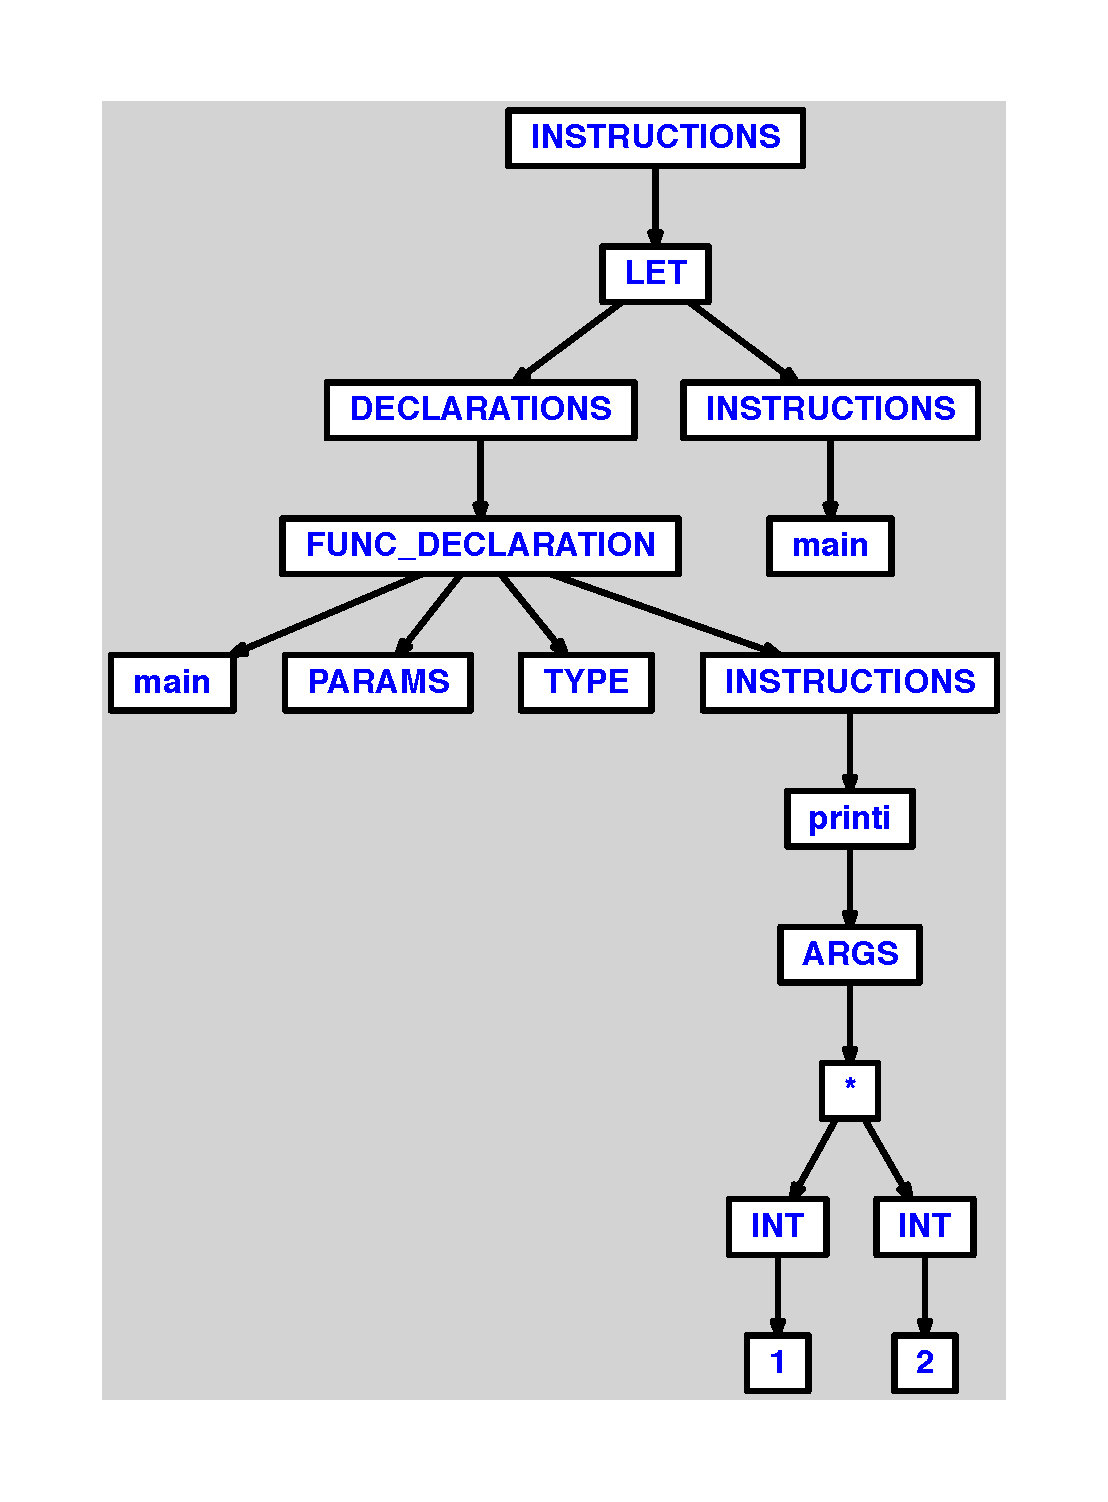
\includegraphics[max width=\textwidth]{ast/ast_41.pdf}\end{figure}\subsubsection{division simple, a 2 termes}
\begin{verbatimtab}
let
	function main() = printi(2/1)
in main() end
\end{verbatimtab}
\begin{figure}[H]\centering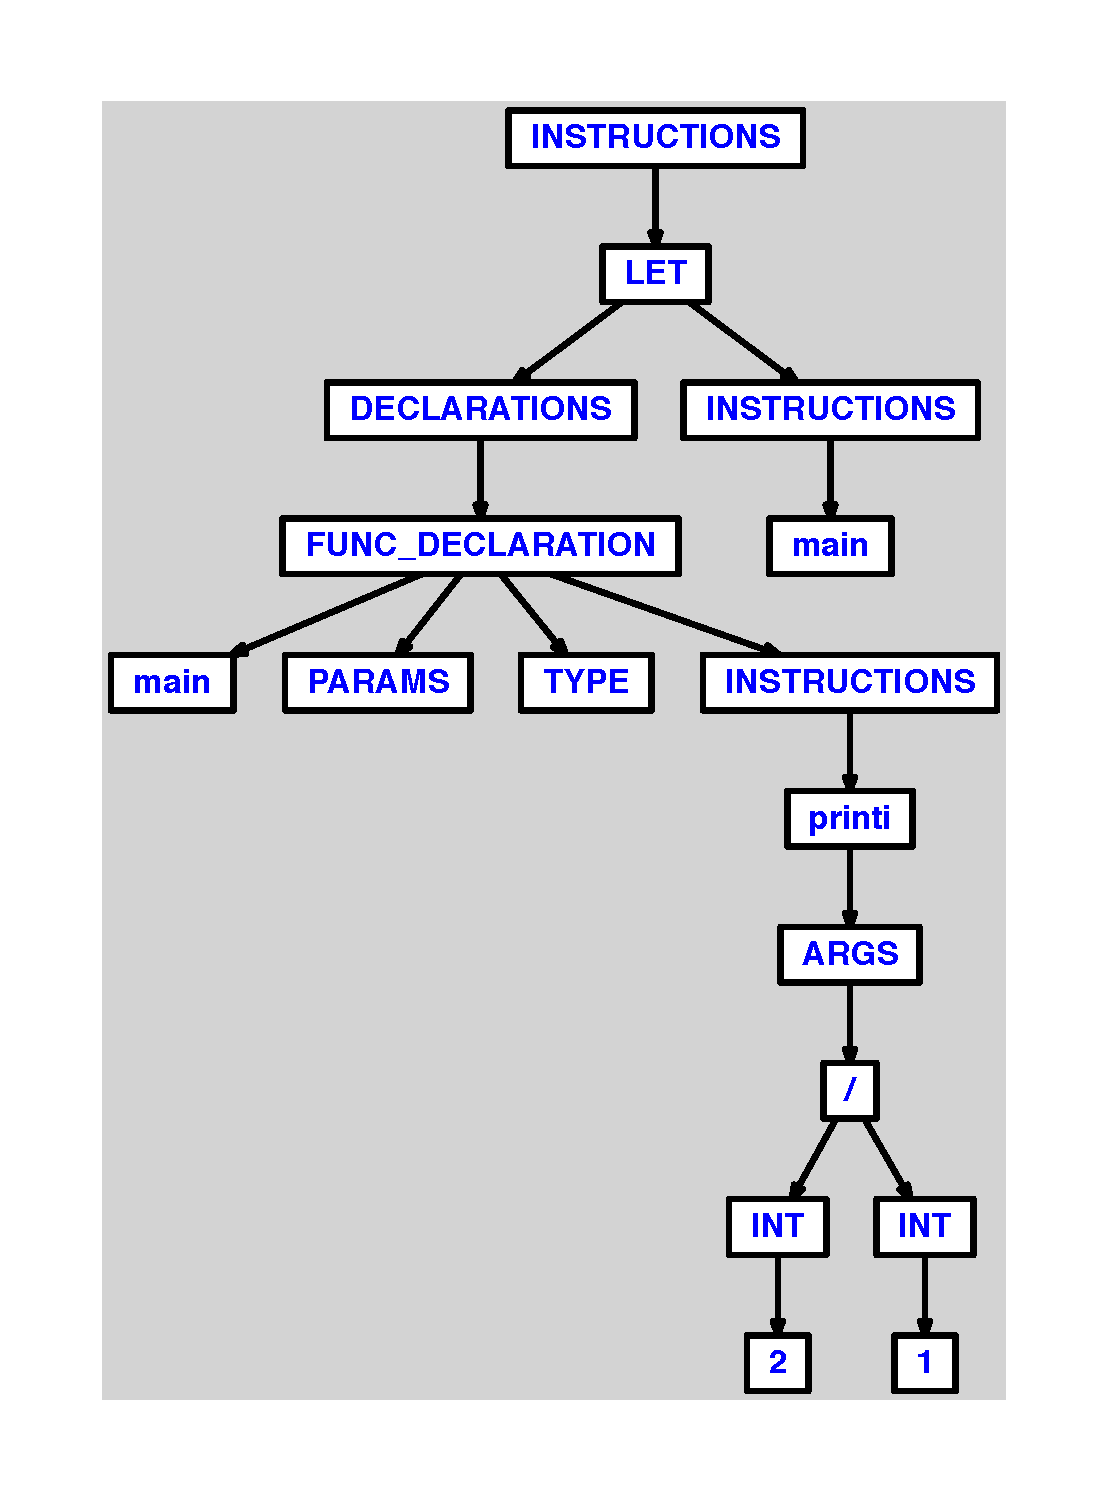
\includegraphics[max width=\textwidth]{ast/ast_42.pdf}\end{figure}\subsubsection{addition a 3 termes}
\begin{verbatimtab}
let
	function main() = printi(1+2+3)
in main() end
\end{verbatimtab}
\begin{figure}[H]\centering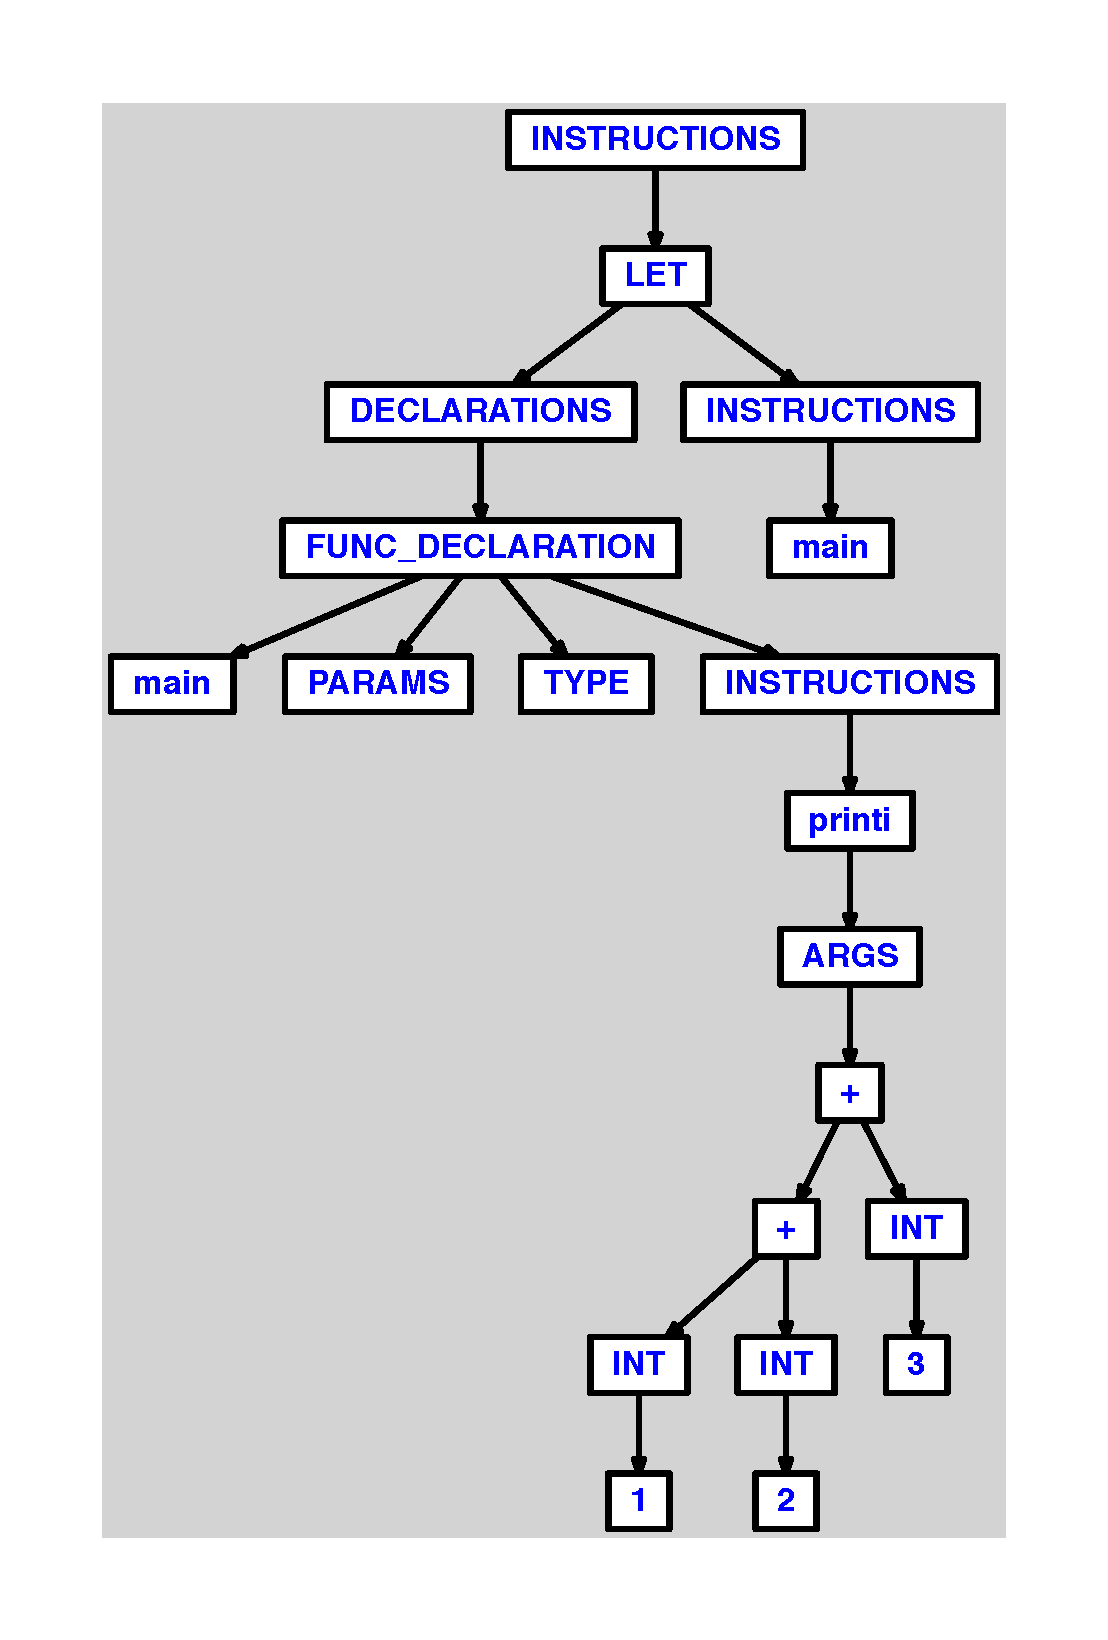
\includegraphics[max width=\textwidth]{ast/ast_43.pdf}\end{figure}\subsubsection{addition suivie de soustraction}
\begin{verbatimtab}
let
	function main() = printi(1+2-3)
in main() end
\end{verbatimtab}
\begin{figure}[H]\centering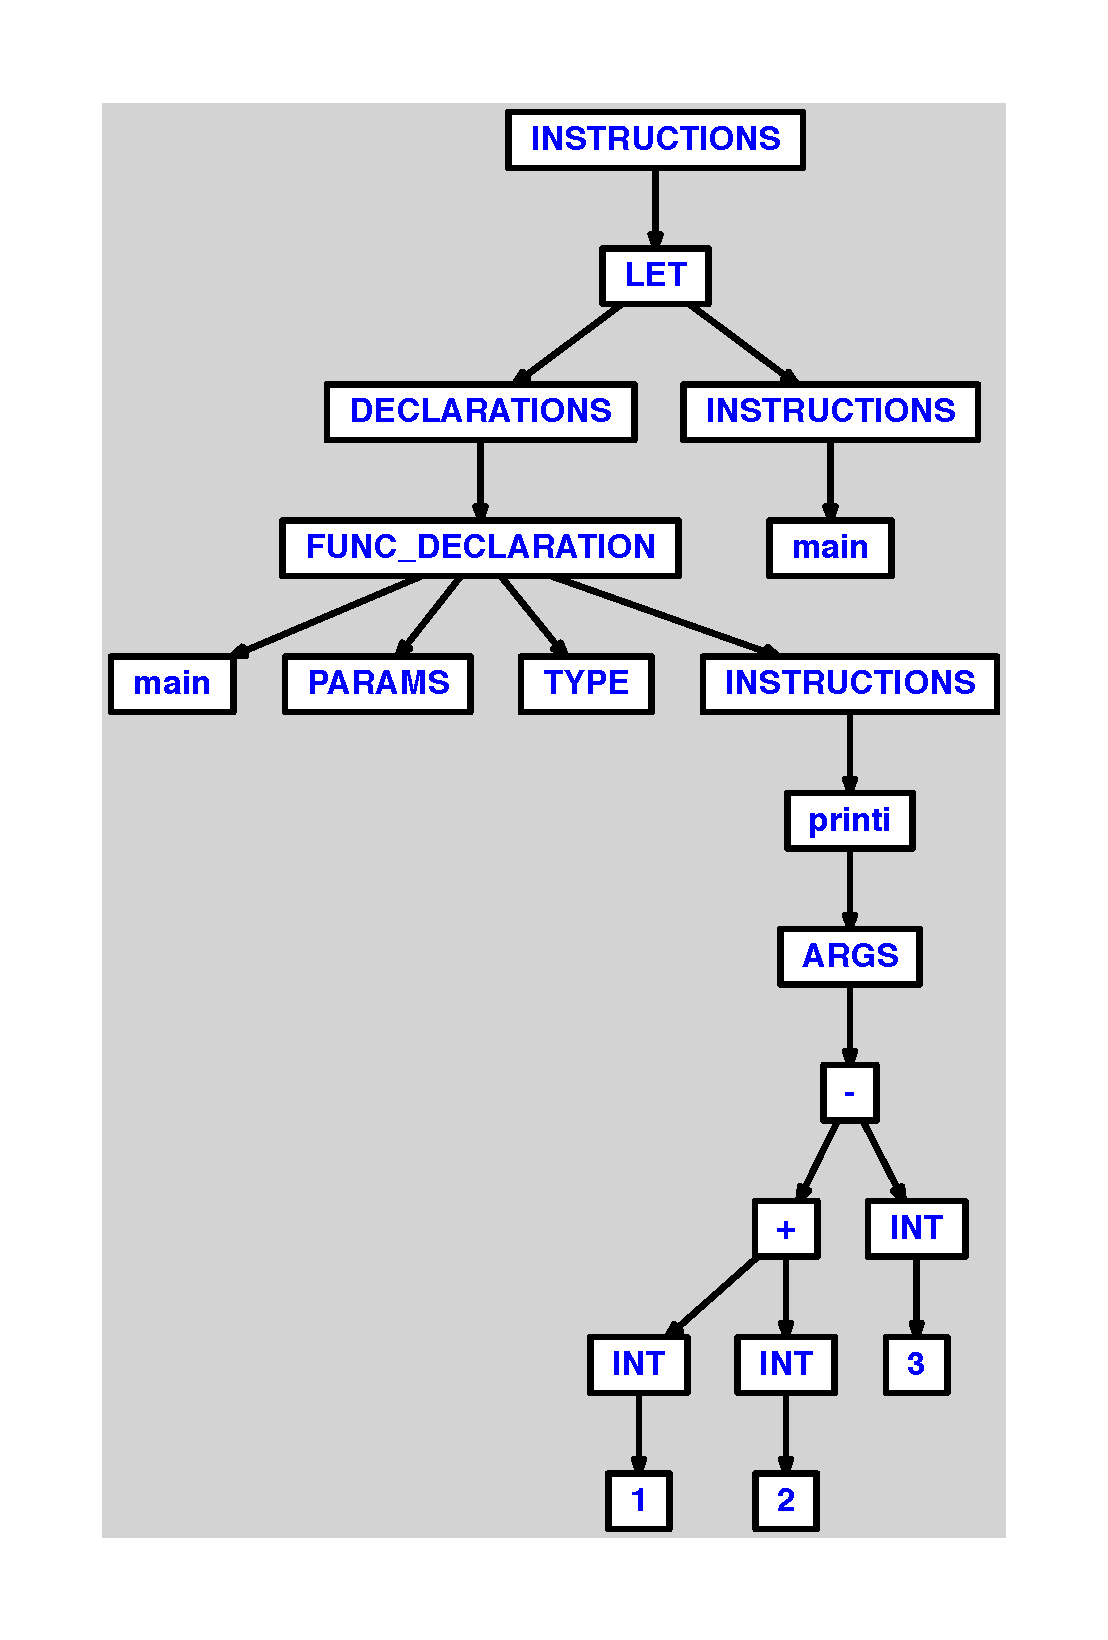
\includegraphics[max width=\textwidth]{ast/ast_44.pdf}\end{figure}\subsubsection{addition suivie de multiplication}
\begin{verbatimtab}
let
	function main() = printi(1+2*3)
in main() end
\end{verbatimtab}
\begin{figure}[H]\centering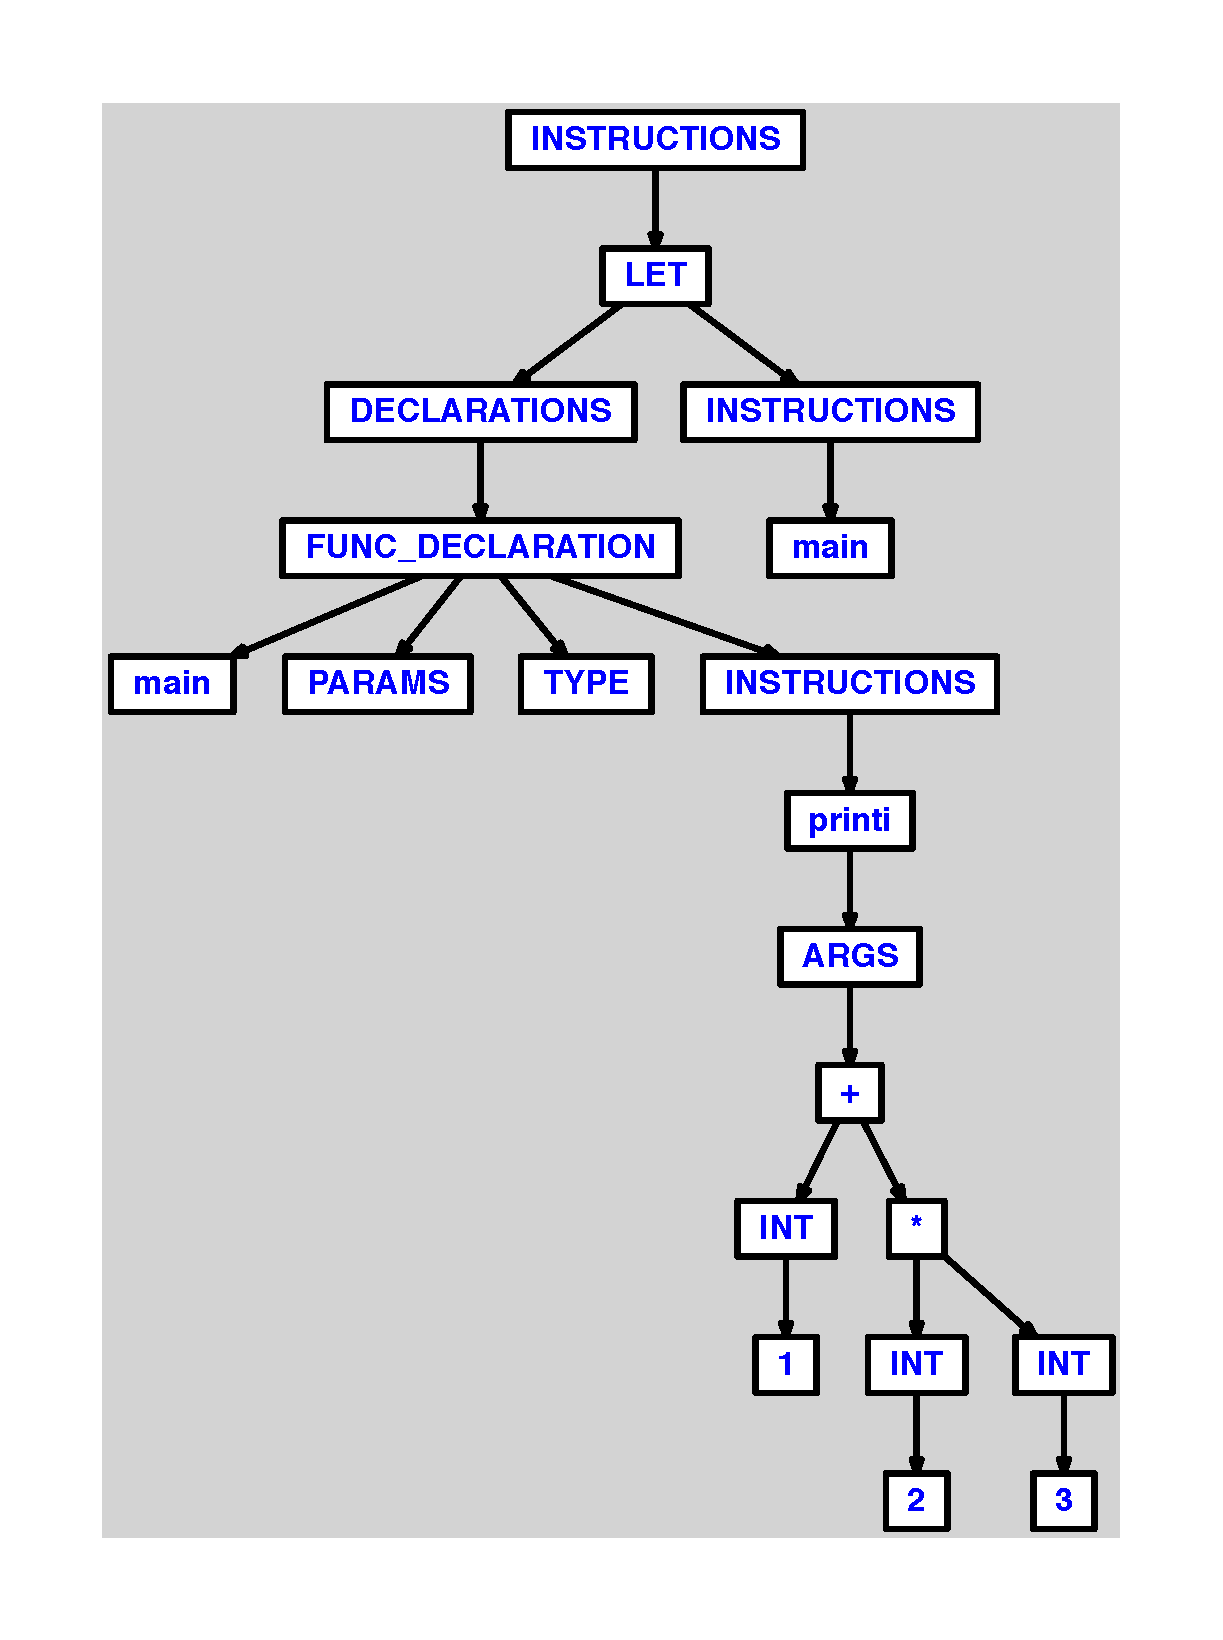
\includegraphics[max width=\textwidth]{ast/ast_45.pdf}\end{figure}\subsubsection{addition suivie de division}
\begin{verbatimtab}
let
	function main() = printi(1+2/3)
in main() end
\end{verbatimtab}
\begin{figure}[H]\centering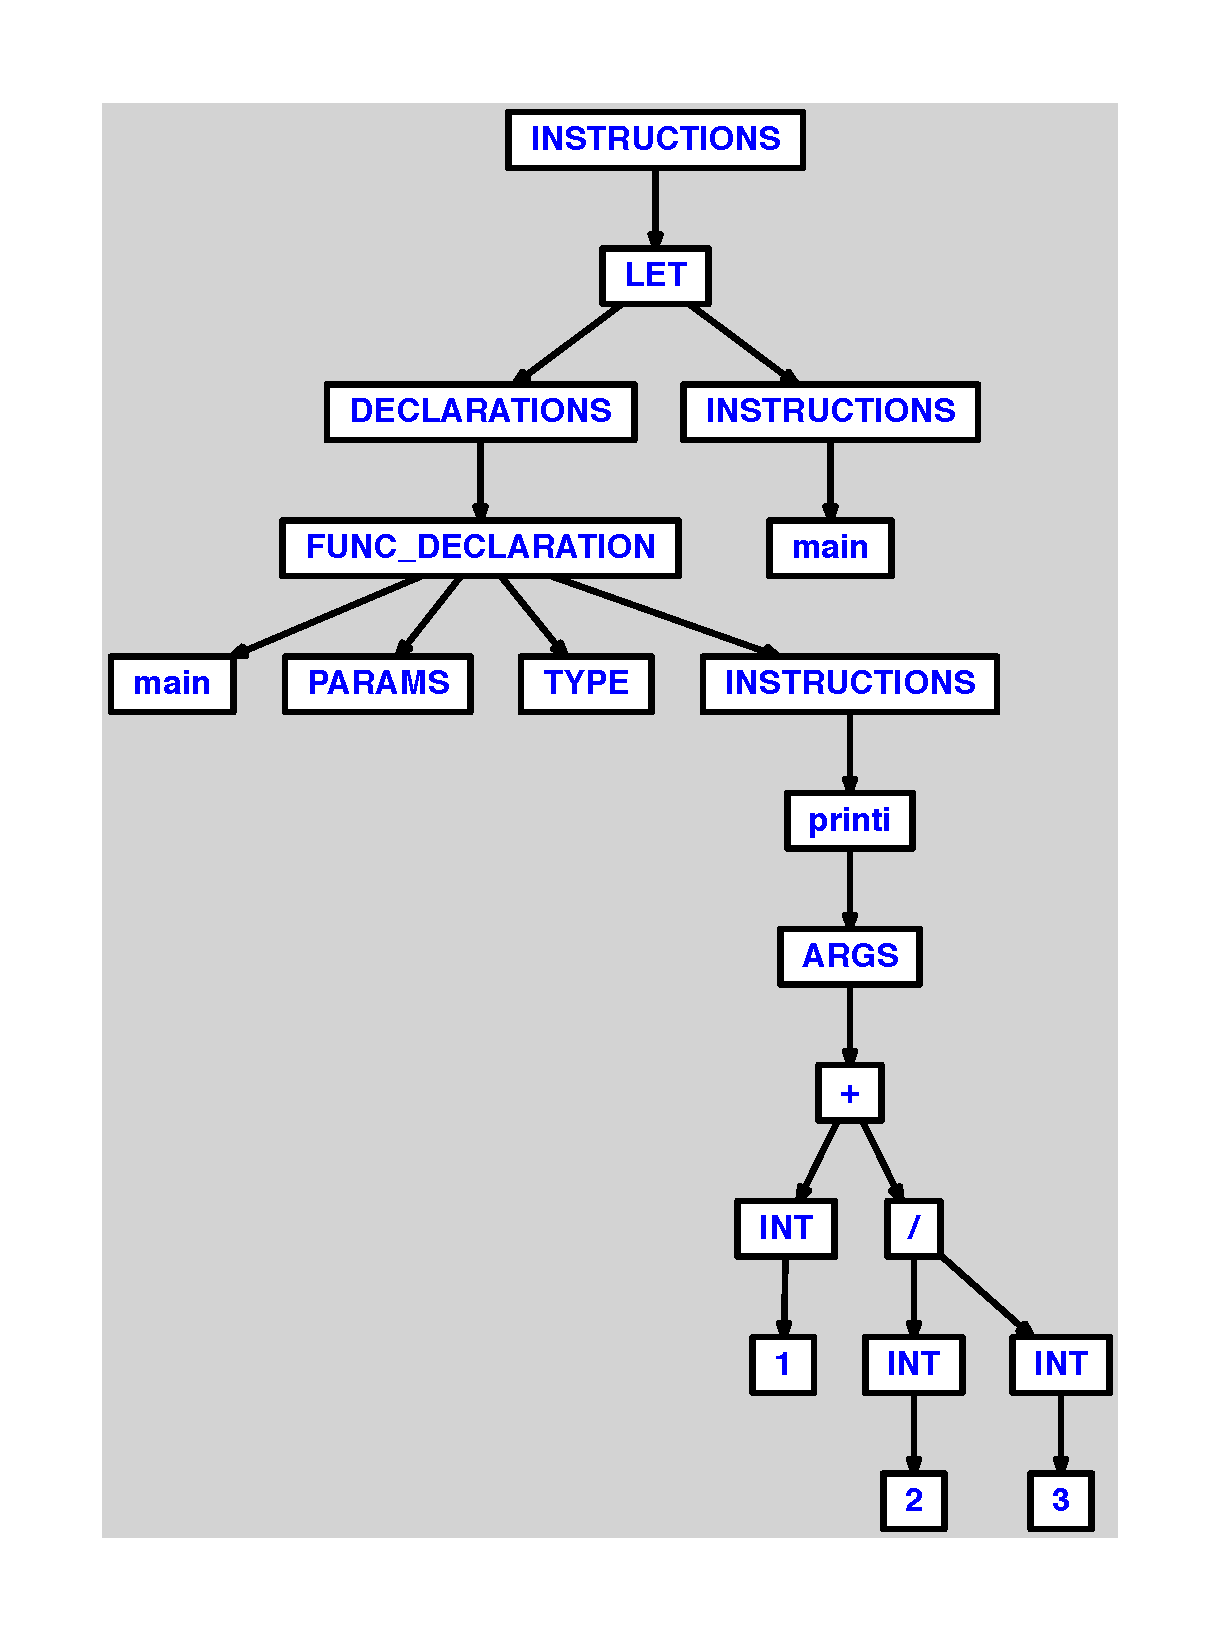
\includegraphics[max width=\textwidth]{ast/ast_46.pdf}\end{figure}\subsubsection{multiplication suivie d'addition}
\begin{verbatimtab}
let
	function main() = printi(1*2+3)
in main() end
\end{verbatimtab}
\begin{figure}[H]\centering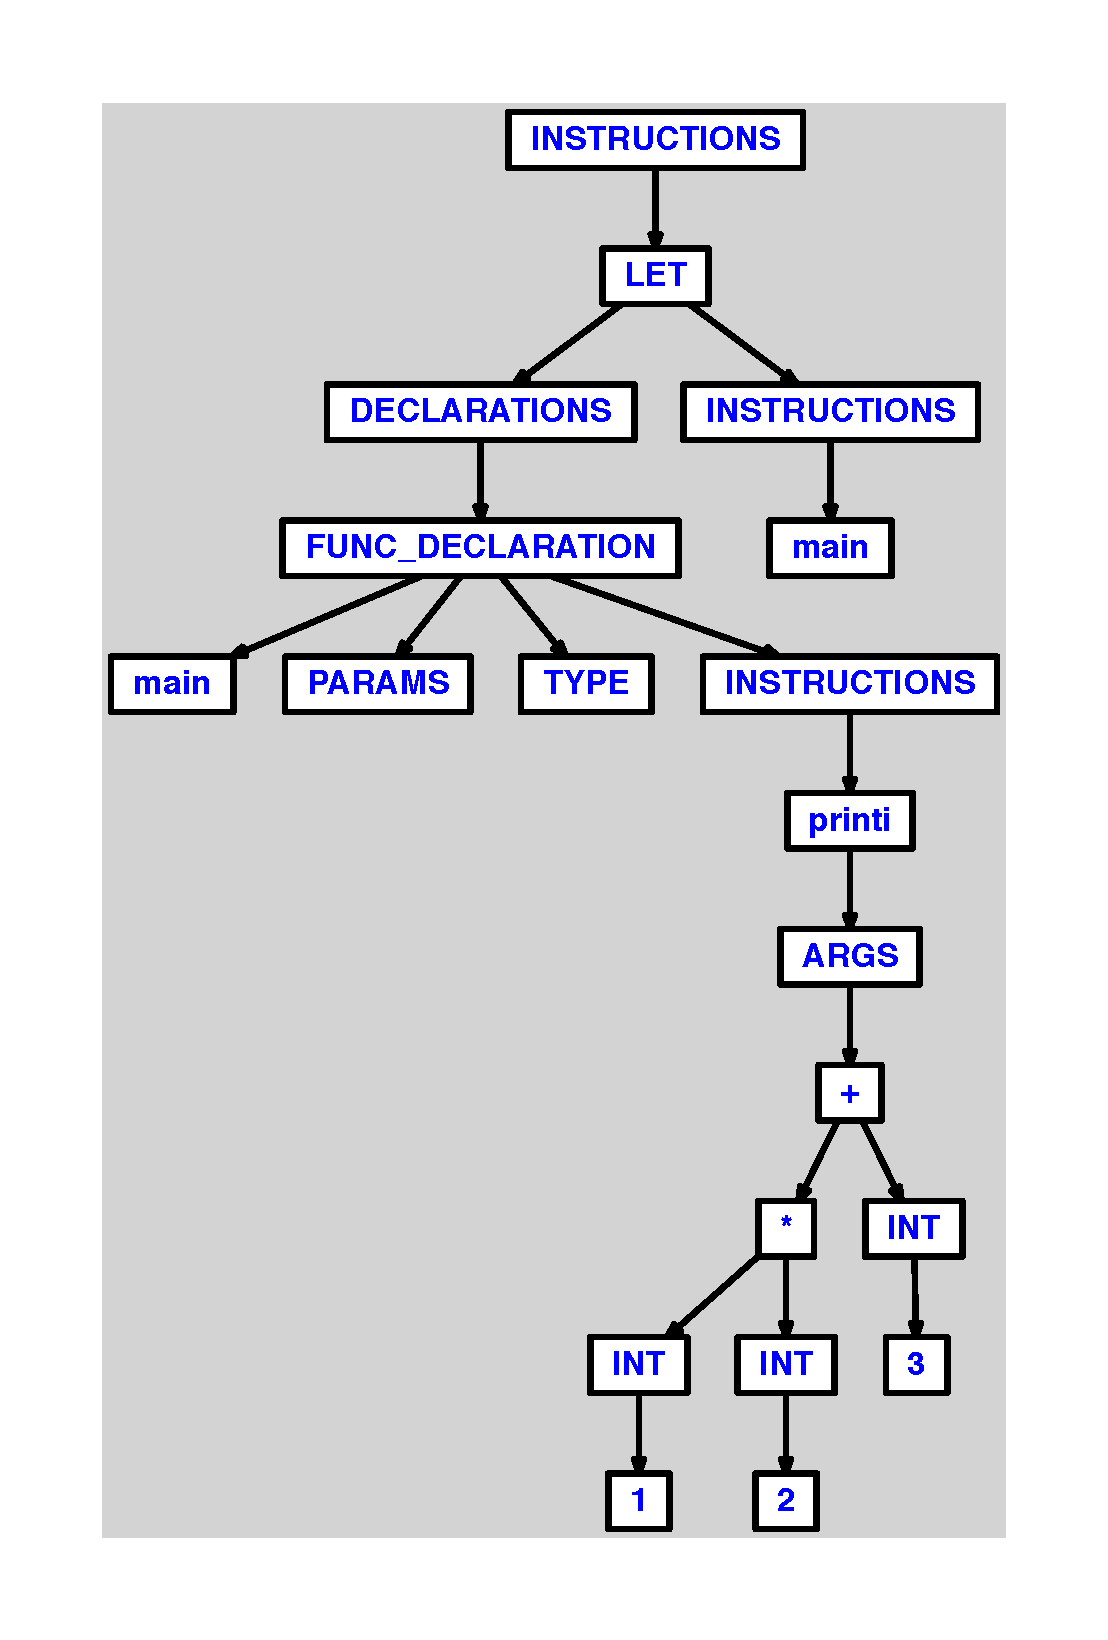
\includegraphics[max width=\textwidth]{ast/ast_47.pdf}\end{figure}\subsubsection{multiplication suivie de soustraction}
\begin{verbatimtab}
let
	function main() = printi(1*2-3)
in main() end
\end{verbatimtab}
\begin{figure}[H]\centering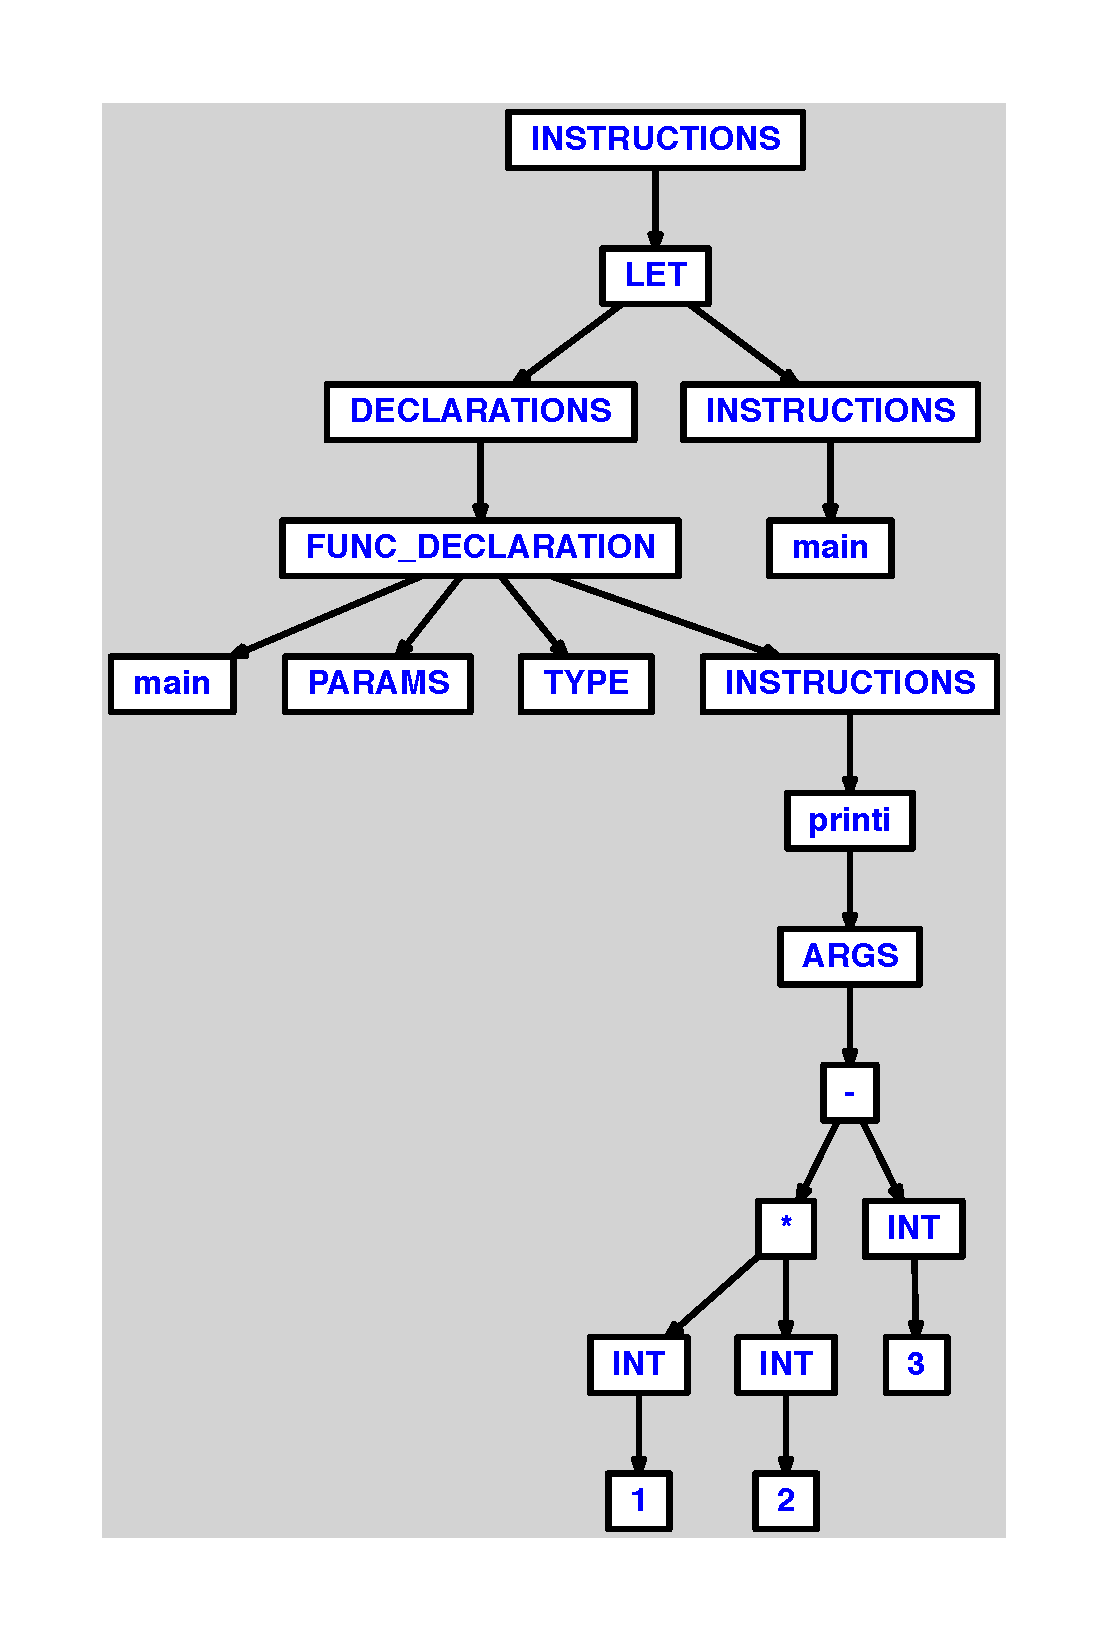
\includegraphics[max width=\textwidth]{ast/ast_48.pdf}\end{figure}\subsubsection{multiplication a 3 termes}
\begin{verbatimtab}
let
	function main() = printi(1*2*3)
in main() end
\end{verbatimtab}
\begin{figure}[H]\centering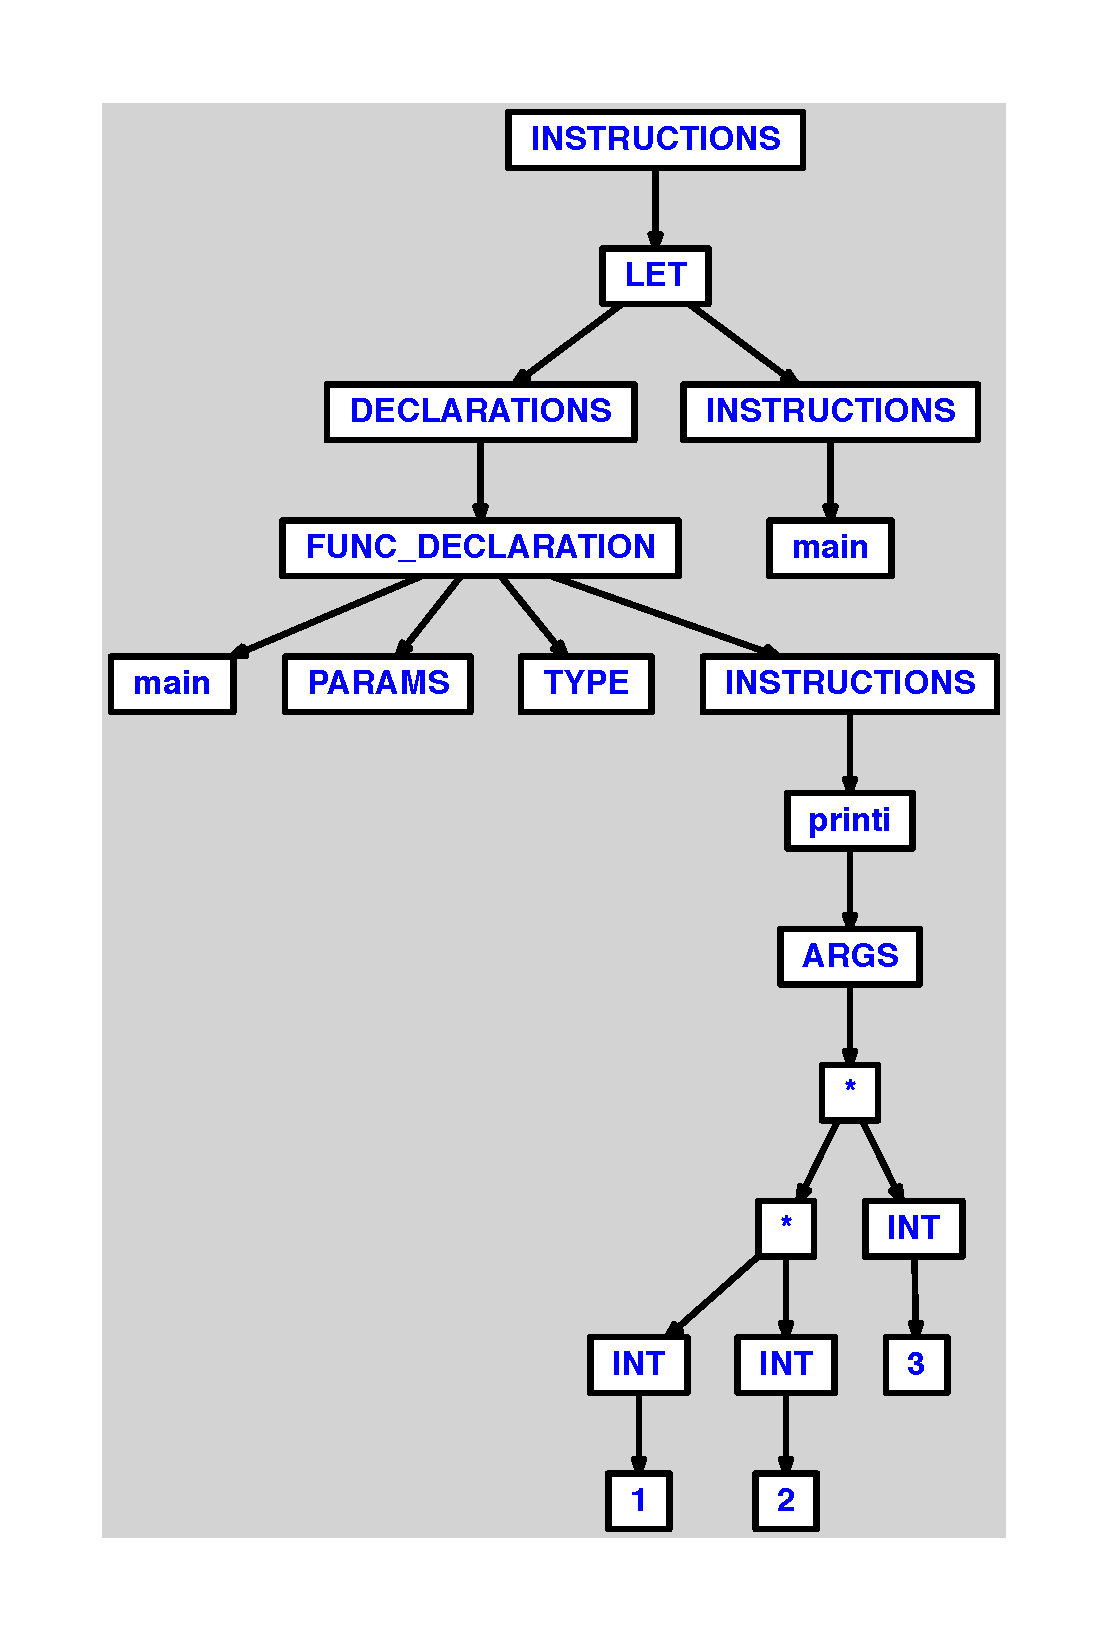
\includegraphics[max width=\textwidth]{ast/ast_49.pdf}\end{figure}\subsubsection{multiplication suivie de division}
\begin{verbatimtab}
let
	function main() = printi(1*2/3)
in main() end
\end{verbatimtab}
\begin{figure}[H]\centering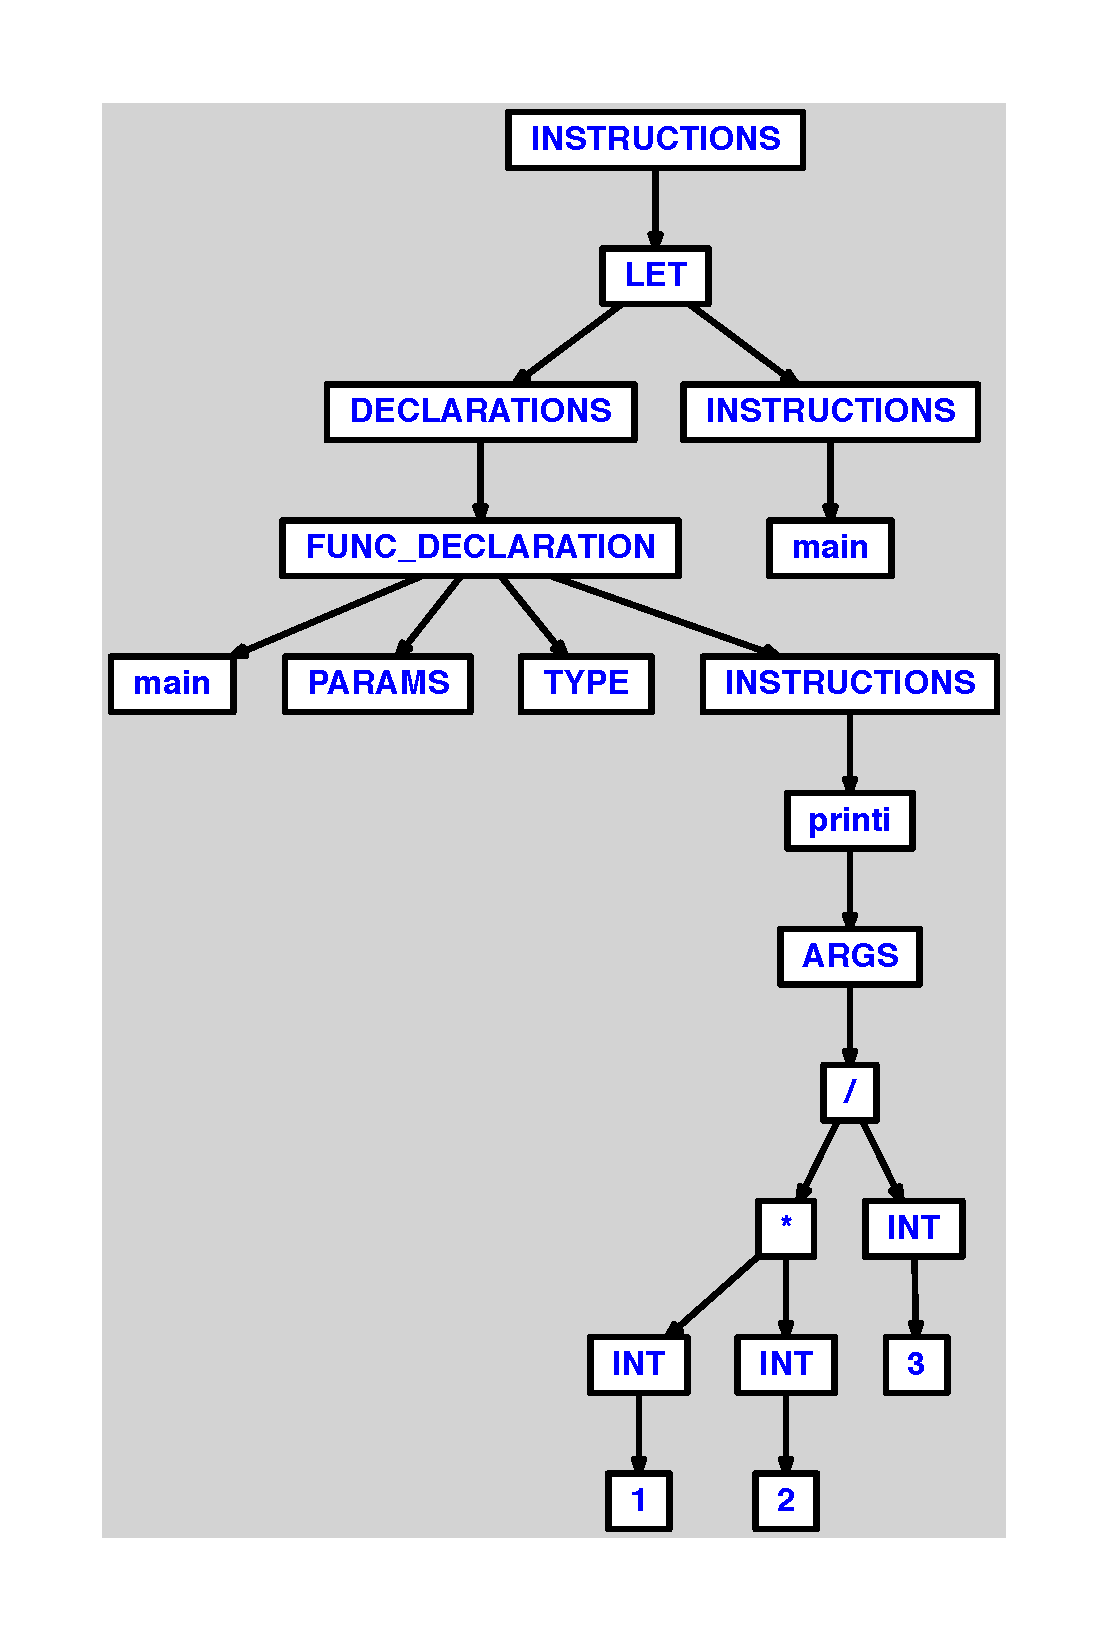
\includegraphics[max width=\textwidth]{ast/ast_50.pdf}\end{figure}\subsubsection{addition simple, a 2 termes, identifies par des variables}
\begin{verbatimtab}
let
	var i := 1
	var j := 2

	function main() = printi(i+j)
in main() end
\end{verbatimtab}
\begin{figure}[H]\centering\includegraphics[max width=\textwidth]{ast/ast_51.pdf}\end{figure}\subsubsection{soustraction simple, a 2 termes, identifies par des variables}
\begin{verbatimtab}
let
	var i := 1
	var j := 2

	function main() = printi(j-i)
in main() end
\end{verbatimtab}
\begin{figure}[H]\centering\includegraphics[max width=\textwidth]{ast/ast_52.pdf}\end{figure}\subsubsection{multiplication simple, a 2 termes, identifies par des variables}
\begin{verbatimtab}
let
	var i := 1
	var j := 2

	function main() = printi(i*j)
in main() end
\end{verbatimtab}
\begin{figure}[H]\centering\includegraphics[max width=\textwidth]{ast/ast_53.pdf}\end{figure}\subsubsection{division simple, a 2 termes, identifies par des variables}
\begin{verbatimtab}
let
	var i := 1
	var j := 2

	function main() = printi(j/i)
in main() end
\end{verbatimtab}
\begin{figure}[H]\centering\includegraphics[max width=\textwidth]{ast/ast_54.pdf}\end{figure}\subsubsection{addition a 3 termes, identifies par des variables}
\begin{verbatimtab}
let
	var i := 1
	var j := 2
	var k := 3

	function main() = printi(i+j+k)
in main() end
\end{verbatimtab}
\begin{figure}[H]\centering\includegraphics[max width=\textwidth]{ast/ast_55.pdf}\end{figure}\subsubsection{addition suivie de soustraction, avec termes identifies par variables}
\begin{verbatimtab}
let
	var i := 1
	var j := 2
	var k := 3

	function main() = printi(i+j-k)
in main() end
\end{verbatimtab}
\begin{figure}[H]\centering\includegraphics[max width=\textwidth]{ast/ast_56.pdf}\end{figure}\subsubsection{addition suivie de multiplication, avec termes identifies par variables}
\begin{verbatimtab}
let
	var i := 1
	var j := 2
	var k := 3

	function main() = printi(i+j*k)
in main() end
\end{verbatimtab}
\begin{figure}[H]\centering\includegraphics[max width=\textwidth]{ast/ast_57.pdf}\end{figure}\subsubsection{addition suivie de division, avec termes identifies par variables}
\begin{verbatimtab}
let
	var i := 1
	var j := 2
	var k := 3

	function main() = printi(i+j/k)
in main() end
\end{verbatimtab}
\begin{figure}[H]\centering\includegraphics[max width=\textwidth]{ast/ast_58.pdf}\end{figure}\subsubsection{multiplication suivie d'addition, avec termes identifies par variables}
\begin{verbatimtab}
let
	var i := 1
	var j := 2
	var k := 3

	function main() = printi(i*j+k)
in main() end
\end{verbatimtab}
\begin{figure}[H]\centering\includegraphics[max width=\textwidth]{ast/ast_59.pdf}\end{figure}\subsubsection{multiplication suivie de soustraction, avec termes identifies par variables}
\begin{verbatimtab}
let
	var i := 1
	var j := 2
	var k := 3

	function main() = printi(i*j-k)
in main() end
\end{verbatimtab}
\begin{figure}[H]\centering\includegraphics[max width=\textwidth]{ast/ast_60.pdf}\end{figure}\subsubsection{multiplication a 3 termes, identifies par des variables}
\begin{verbatimtab}
let
	var i := 1
	var j := 2
	var k := 3

	function main() = printi(i*j*k)
in main() end
\end{verbatimtab}
\begin{figure}[H]\centering\includegraphics[max width=\textwidth]{ast/ast_61.pdf}\end{figure}\subsubsection{mutliplication suivie de division, avec termes identifies par variables}
\begin{verbatimtab}
let
	var i := 1
	var j := 2
	var k := 3

	function main() = printi(i*j/k)
in main() end
\end{verbatimtab}
\begin{figure}[H]\centering\includegraphics[max width=\textwidth]{ast/ast_62.pdf}\end{figure}\subsubsection{addition simple, a 2 termes, dont un ayant moins unaire}
\begin{verbatimtab}
let
	function main() = printi(-1+2)
in main() end
\end{verbatimtab}
\begin{figure}[H]\centering\includegraphics[max width=\textwidth]{ast/ast_63.pdf}\end{figure}\subsubsection{soustraction simple, a 2 termes, dont ayant moins unaire}
\begin{verbatimtab}
let
	function main() = printi(-2-1)
in main() end
\end{verbatimtab}
\begin{figure}[H]\centering\includegraphics[max width=\textwidth]{ast/ast_64.pdf}\end{figure}\subsubsection{multiplication simple, a 2 termes, dont un ayant moins unaire}
\begin{verbatimtab}
let
	function main() = printi(-1*2)
in main() end
\end{verbatimtab}
\begin{figure}[H]\centering\includegraphics[max width=\textwidth]{ast/ast_65.pdf}\end{figure}\subsubsection{division simple, a 2 termes, dont un ayant moins unaire}
\begin{verbatimtab}
let
	function main() = printi(-2/1)
in main() end
\end{verbatimtab}
\begin{figure}[H]\centering\includegraphics[max width=\textwidth]{ast/ast_66.pdf}\end{figure}\subsubsection{addition a 3 termes, dont un ayant moins unaire}
\begin{verbatimtab}
let
	function main() = printi(-1+2+3)
in main() end
\end{verbatimtab}
\begin{figure}[H]\centering\includegraphics[max width=\textwidth]{ast/ast_67.pdf}\end{figure}\subsubsection{addition suivie de soustraction, avec un terme ayant moins unaire}
\begin{verbatimtab}
let
	function main() = printi(-1+2-3)
in main() end
\end{verbatimtab}
\begin{figure}[H]\centering\includegraphics[max width=\textwidth]{ast/ast_68.pdf}\end{figure}\subsubsection{addition suivie de multiplication, avec un terme ayant moins unaire}
\begin{verbatimtab}
let
	function main() = printi(-1+2*3)
in main() end
\end{verbatimtab}
\begin{figure}[H]\centering\includegraphics[max width=\textwidth]{ast/ast_69.pdf}\end{figure}\subsubsection{addition suivie de division, avec un terme ayant moins unaire}
\begin{verbatimtab}
let
	function main() = printi(-1+2/3)
in main() end
\end{verbatimtab}
\begin{figure}[H]\centering\includegraphics[max width=\textwidth]{ast/ast_70.pdf}\end{figure}\subsubsection{multiplication suivie d'addition, dont un terme ayant moins unaire}
\begin{verbatimtab}
let
	function main() = printi(-1*2+3)
in main() end
\end{verbatimtab}
\begin{figure}[H]\centering\includegraphics[max width=\textwidth]{ast/ast_71.pdf}\end{figure}\subsubsection{multiplication suivie de soustraction, dont un terme ayant moins unaire}
\begin{verbatimtab}
let
	function main() = printi(-1*2-3)
in main() end
\end{verbatimtab}
\begin{figure}[H]\centering\includegraphics[max width=\textwidth]{ast/ast_72.pdf}\end{figure}\subsubsection{multiplication a 3 termes, dont un ayant moins unaire}
\begin{verbatimtab}
let
	function main() = printi(-1*2*3)
in main() end
\end{verbatimtab}
\begin{figure}[H]\centering\includegraphics[max width=\textwidth]{ast/ast_73.pdf}\end{figure}\subsubsection{multiplication suivie de division, dont un terme ayant moins unaire}
\begin{verbatimtab}
let
	function main() = printi(-1*2/3)
in main() end
\end{verbatimtab}
\begin{figure}[H]\centering\includegraphics[max width=\textwidth]{ast/ast_74.pdf}\end{figure}\subsubsection{addition simple, a 2 termes, identifies par des variables, dont une ayant moins unaire}
\begin{verbatimtab}
let
	var i := 1
	var j := 2

	function main() = printi(-i+j)
in main() end
\end{verbatimtab}
\begin{figure}[H]\centering\includegraphics[max width=\textwidth]{ast/ast_75.pdf}\end{figure}\subsubsection{soustraction simple, a 2 termes, identifies par des variables, dont une ayant moins unaire}
\begin{verbatimtab}
let
	var i := 1
	var j := 2

	function main() = printi(-j-i)
in main() end
\end{verbatimtab}
\begin{figure}[H]\centering\includegraphics[max width=\textwidth]{ast/ast_76.pdf}\end{figure}\subsubsection{multiplication simple, a 2 termes, identifies par des variables, dont une ayant moins unaire}
\begin{verbatimtab}
let
	var i := 1
	var j := 2

	function main() = printi(-i*j)
in main() end
\end{verbatimtab}
\begin{figure}[H]\centering\includegraphics[max width=\textwidth]{ast/ast_77.pdf}\end{figure}\subsubsection{division simple, a 2 termes, identifies par des variables, dont une ayant moins unaire}
\begin{verbatimtab}
let
	var i := 1
	var j := 2

	function main() = printi(-j/i)
in main() end
\end{verbatimtab}
\begin{figure}[H]\centering\includegraphics[max width=\textwidth]{ast/ast_78.pdf}\end{figure}\subsubsection{addition a 3 termes, identifies par des variables, dont une ayant moins unaire}
\begin{verbatimtab}
let
	var i := 1
	var j := 2
	var k := 3

	function main() = printi(-i+j+k)
in main() end
\end{verbatimtab}
\begin{figure}[H]\centering\includegraphics[max width=\textwidth]{ast/ast_79.pdf}\end{figure}\subsubsection{addition suivie de soustraction, avec termes identifies par variables, dont une ayant moins unaire}
\begin{verbatimtab}
let
	var i := 1
	var j := 2
	var k := 3

	function main() = printi(-i+j-k)
in main() end
\end{verbatimtab}
\begin{figure}[H]\centering\includegraphics[max width=\textwidth]{ast/ast_80.pdf}\end{figure}\subsubsection{addition suivie de multiplication, avec termes identifies par variables, dont une ayant moins unaire}
\begin{verbatimtab}
let
	var i := 1
	var j := 2
	var k := 3

	function main() = printi(-i+j*k)
in main() end
\end{verbatimtab}
\begin{figure}[H]\centering\includegraphics[max width=\textwidth]{ast/ast_81.pdf}\end{figure}\subsubsection{addition suivie de division, avec termes identifies par variables, dont une ayant moins unaire}
\begin{verbatimtab}
let
	var i := 1
	var j := 2
	var k := 3

	function main() = printi(-i+j/k)
in main() end
\end{verbatimtab}
\begin{figure}[H]\centering\includegraphics[max width=\textwidth]{ast/ast_82.pdf}\end{figure}\subsubsection{multiplication suivie d'addition, avec termes identifies par variables, dont une ayant moins unaire}
\begin{verbatimtab}
let
	var i := 1
	var j := 2
	var k := 3

	function main() = printi(-i*j+k)
in main() end
\end{verbatimtab}
\begin{figure}[H]\centering\includegraphics[max width=\textwidth]{ast/ast_83.pdf}\end{figure}\subsubsection{multiplication suivie de soustraction, avec termes identifies par variables, dont une ayant moins unaire}
\begin{verbatimtab}
let
	var i := 1
	var j := 2
	var k := 3

	function main() = printi(-i*j-k)
in main() end
\end{verbatimtab}
\begin{figure}[H]\centering\includegraphics[max width=\textwidth]{ast/ast_84.pdf}\end{figure}\subsubsection{multiplication a 3 termes, identifies par des variables, dont une ayant moins unaire}
\begin{verbatimtab}
let
	var i := 1
	var j := 2
	var k := 3

	function main() = printi(-i*j*k)
in main() end
\end{verbatimtab}
\begin{figure}[H]\centering\includegraphics[max width=\textwidth]{ast/ast_85.pdf}\end{figure}\subsubsection{mutliplication suivie de division, avec termes identifies par variables, dont une ayant moins unaire}
\begin{verbatimtab}
let
	var i := 1
	var j := 2
	var k := 3

	function main() = printi(-i*j/k)
in main() end
\end{verbatimtab}
\begin{figure}[H]\centering\includegraphics[max width=\textwidth]{ast/ast_86.pdf}\end{figure}\subsubsection{addition a 3 termes, avec parenthesage des 2 termes a droite}
\begin{verbatimtab}
let function main() = printi(1+(2+3)) in main() end
\end{verbatimtab}
\begin{figure}[H]\centering\includegraphics[max width=\textwidth]{ast/ast_87.pdf}\end{figure}\subsubsection{addition suivie de soustraction, avec parenthesage des 2 termes a droite}
\begin{verbatimtab}
let function main() = printi(1+(2-3)) in main() end
\end{verbatimtab}
\begin{figure}[H]\centering\includegraphics[max width=\textwidth]{ast/ast_88.pdf}\end{figure}\subsubsection{addition suivie de multiplication, avec parenthesage des 2 termes a droite}
\begin{verbatimtab}
let function main() = printi(1+(2*3)) in main() end
\end{verbatimtab}
\begin{figure}[H]\centering\includegraphics[max width=\textwidth]{ast/ast_89.pdf}\end{figure}\subsubsection{addition suivie de division, avec parenthesage des 2 termes a droite}
\begin{verbatimtab}
let function main() = printi(1+(2/3)) in main() end
\end{verbatimtab}
\begin{figure}[H]\centering\includegraphics[max width=\textwidth]{ast/ast_90.pdf}\end{figure}\subsubsection{multiplication suivie d'addition, avec parenthesage des 2 termes a droite}
\begin{verbatimtab}
let function main() = printi(1*(2+3)) in main() end
\end{verbatimtab}
\begin{figure}[H]\centering\includegraphics[max width=\textwidth]{ast/ast_91.pdf}\end{figure}\subsubsection{multiplication suivie de soustraction, avec parenthesage des 2 termes a droite}
\begin{verbatimtab}
let function main() = printi(1*(2-3)) in main() end
\end{verbatimtab}
\begin{figure}[H]\centering\includegraphics[max width=\textwidth]{ast/ast_92.pdf}\end{figure}\subsubsection{multiplication a 3 termes, avec parenthesage des 2 termes a droite}
\begin{verbatimtab}
let function main() = printi(1*(2*3)) in main() end
\end{verbatimtab}
\begin{figure}[H]\centering\includegraphics[max width=\textwidth]{ast/ast_93.pdf}\end{figure}\subsubsection{multiplication suivie de vision, avec parenthesage des 2 termes a droite}
\begin{verbatimtab}
let function main() = printi(1*(2/3)) in main() end
\end{verbatimtab}
\begin{figure}[H]\centering\includegraphics[max width=\textwidth]{ast/ast_94.pdf}\end{figure}\subsubsection{addition a 3 termes, avec parenthesage des 2 termes a gauche}
\begin{verbatimtab}
let function main() = printi((1+2)+3) in main() end
\end{verbatimtab}
\begin{figure}[H]\centering\includegraphics[max width=\textwidth]{ast/ast_95.pdf}\end{figure}\subsubsection{addition suivie de soustraction, avec parenthesage des 2 termes a gauche}
\begin{verbatimtab}
let function main() = printi((1+2)-3) in main() end
\end{verbatimtab}
\begin{figure}[H]\centering\includegraphics[max width=\textwidth]{ast/ast_96.pdf}\end{figure}\subsubsection{addition suivie de multiplication, avec parenthesage des 2 termes a gauche}
\begin{verbatimtab}
let function main() = printi((1+2)*3) in main() end
\end{verbatimtab}
\begin{figure}[H]\centering\includegraphics[max width=\textwidth]{ast/ast_97.pdf}\end{figure}\subsubsection{addition suivie de division, avec parenthesage des 2 termes a gauche}
\begin{verbatimtab}
let function main() = printi((1+2)/3) in main() end
\end{verbatimtab}
\begin{figure}[H]\centering\includegraphics[max width=\textwidth]{ast/ast_98.pdf}\end{figure}\subsubsection{multiplication suivie d'addition, avec parenthesage des 2 termes a gauche}
\begin{verbatimtab}
let function main() = printi((1*2)+3) in main() end
\end{verbatimtab}
\begin{figure}[H]\centering\includegraphics[max width=\textwidth]{ast/ast_99.pdf}\end{figure}\subsubsection{multiplication suivie de soustraction, avec parenthesage des 2 termes a gauche}
\begin{verbatimtab}
let function main() = printi((1*2)-3) in main() end
\end{verbatimtab}
\begin{figure}[H]\centering\includegraphics[max width=\textwidth]{ast/ast_100.pdf}\end{figure}\subsubsection{multiplication a 3 termes, avec parenthesage des 2 termes a gauche}
\begin{verbatimtab}
let function main() = printi((1*2)*3) in main() end
\end{verbatimtab}
\begin{figure}[H]\centering\includegraphics[max width=\textwidth]{ast/ast_101.pdf}\end{figure}\subsubsection{multiplication suivie de division, avec parenthesage des 2 termes a gauche}
\begin{verbatimtab}
let function min() = printi((1*2)/3) in main() end
\end{verbatimtab}
\begin{figure}[H]\centering\includegraphics[max width=\textwidth]{ast/ast_102.pdf}\end{figure}\subsubsection{multiplication de 2 additions parenthesees}
\begin{verbatimtab}
let function main() = printi((1+2)*(2+3)) in main() end */
\end{verbatimtab}
\begin{figure}[H]\centering\includegraphics[max width=\textwidth]{ast/ast_103.pdf}\end{figure}\subsubsection{multiplication de 3 additions parenthesees}
\begin{verbatimtab}
let function main() = printi((1+2)*(2+3)*(3+4)) in main() end
\end{verbatimtab}
\begin{figure}[H]\centering\includegraphics[max width=\textwidth]{ast/ast_104.pdf}\end{figure}\subsubsection{division de 2 soustractions parenthesees}
\begin{verbatimtab}
let function main() = printi((2-1)/(3-2)) in main() end
\end{verbatimtab}
\begin{figure}[H]\centering\includegraphics[max width=\textwidth]{ast/ast_105.pdf}\end{figure}\subsubsection{division de 3 soustractions parenthesees}
\begin{verbatimtab}
let function main() = printi((2-1)/(3-2)/(4-3)) in main() end
\end{verbatimtab}
\begin{figure}[H]\centering\includegraphics[max width=\textwidth]{ast/ast_106.pdf}\end{figure}\subsubsection{addition de 2 multiplications parenthesees}
\begin{verbatimtab}
let function main() = printi((1*2)+(2*3)) in main() end
\end{verbatimtab}
\begin{figure}[H]\centering\includegraphics[max width=\textwidth]{ast/ast_107.pdf}\end{figure}\subsubsection{addition de 3 multiplications parenthesees}
\begin{verbatimtab}
let function main() = printi((1*2)+(2*3)+(3*4)) in main() end
\end{verbatimtab}
\begin{figure}[H]\centering\includegraphics[max width=\textwidth]{ast/ast_108.pdf}\end{figure}\subsubsection{soustraction de 2 divisions parenthesees}
\begin{verbatimtab}
let function main() = printi((2/1)-(4/2) in main() end
\end{verbatimtab}
\begin{figure}[H]\centering\includegraphics[max width=\textwidth]{ast/ast_109.pdf}\end{figure}\subsubsection{soustraction de 3 divisions parenthesees}
\begin{verbatimtab}
let function main() = printi((2/1)-(4/2)-(8/4)) in main() end
\end{verbatimtab}
\begin{figure}[H]\centering\includegraphics[max width=\textwidth]{ast/ast_110.pdf}\end{figure}\subsubsection{addition a 3 termes identifies par variables, avec parenthesage des 2 variables a droite}
\begin{verbatimtab}
let
	var i := 1
	var j := 2
	var k := 3

	function main() = printi(i+(j+k))
in main() end
\end{verbatimtab}
\begin{figure}[H]\centering\includegraphics[max width=\textwidth]{ast/ast_111.pdf}\end{figure}\subsubsection{addition suivie de soustraction, avec termes identifies par variables et parenthesage des 2 variables a droite}
\begin{verbatimtab}
let
	var i := 1
	var j := 2
	var k := 3

	function main() = printi(i+(j-k))
in main() end
\end{verbatimtab}
\begin{figure}[H]\centering\includegraphics[max width=\textwidth]{ast/ast_112.pdf}\end{figure}\subsubsection{addition suivie de multiplication, avec termes identifies par variables et parenthesage des 2 variables a droite}
\begin{verbatimtab}
let
	var i := 1
	var j := 2
	var k := 3

	function main() = printi(i+(j*k))
in main() end
\end{verbatimtab}
\begin{figure}[H]\centering\includegraphics[max width=\textwidth]{ast/ast_113.pdf}\end{figure}\subsubsection{addition suivie de division, avec termes identifies par variables et parenthesage des 2 variables a droite}
\begin{verbatimtab}
let
	var i := 1
	var j := 2
	var k := 3

	function main() = printi(i+(j/k))
in main() end
\end{verbatimtab}
\begin{figure}[H]\centering\includegraphics[max width=\textwidth]{ast/ast_114.pdf}\end{figure}\subsubsection{multiplication suivie d'addition, avec termes identifies par variables et parenthesage des 2 variables a droite}
\begin{verbatimtab}
let
	var i := 1
	var j := 2
	var k := 3

	function main() = printi(i*(j+k))
in main() end
\end{verbatimtab}
\begin{figure}[H]\centering\includegraphics[max width=\textwidth]{ast/ast_115.pdf}\end{figure}\subsubsection{multiplication suivie de soustraction, avec termes identifies par variables et parenthesage des 2 variables a droite}
\begin{verbatimtab}
let
	var i := 1
	var j := 2
	var k := 3

	function main() = printi(i*(j-k))
in main() end
\end{verbatimtab}
\begin{figure}[H]\centering\includegraphics[max width=\textwidth]{ast/ast_116.pdf}\end{figure}\subsubsection{multiplication a 3 termes identifies par variables, avec parenthesage des 2 variables a droite}
\begin{verbatimtab}
let
	var i := 1
	var j := 2
	var k := 3

	function main() = printi(i*(j*k))
in main() end
\end{verbatimtab}
\begin{figure}[H]\centering\includegraphics[max width=\textwidth]{ast/ast_117.pdf}\end{figure}\subsubsection{multiplication suivie de division, avec termes identifies par variables et parenthesage des 2 variables a droite}
\begin{verbatimtab}
let
	var i := 1
	var j := 2
	var k := 3

	function main() = printi(i*(j/k))
in main() end
\end{verbatimtab}
\begin{figure}[H]\centering\includegraphics[max width=\textwidth]{ast/ast_118.pdf}\end{figure}\subsubsection{addition a 3 termes identifies par variables, avec parenthesage des 2 variables a gauche}
\begin{verbatimtab}
let
	var i := 1
	var j := 2
	var k := 3

	function main() = printi((i+j)+k)
in main() end
\end{verbatimtab}
\begin{figure}[H]\centering\includegraphics[max width=\textwidth]{ast/ast_119.pdf}\end{figure}\subsubsection{addition suivie de soustraction, avec termes identifies par variables et parenthesage des 2 variables a gauche}
\begin{verbatimtab}
let
	var i := 1
	var j := 2
	var k := 3

	function main() = printi((i+j)-k)
in main() end
\end{verbatimtab}
\begin{figure}[H]\centering\includegraphics[max width=\textwidth]{ast/ast_120.pdf}\end{figure}\subsubsection{addition suivie de multiplication, avec termes identifies par variables et parenthesage des 2 variables a gauche}
\begin{verbatimtab}
let
	var i := 1
	var j := 2
	var k := 3

	function main() = printi((i+j)*k)
in main() end
\end{verbatimtab}
\begin{figure}[H]\centering\includegraphics[max width=\textwidth]{ast/ast_121.pdf}\end{figure}\subsubsection{addition suivie de division, avec termes identifies par variables et parenthesage des 2 variables a gauche}
\begin{verbatimtab}
let
	var i := 1
	var j := 2
	var k := 3

	function main() = printi((i+j)/k)
in main() end
\end{verbatimtab}
\begin{figure}[H]\centering\includegraphics[max width=\textwidth]{ast/ast_122.pdf}\end{figure}\subsubsection{multiplication suivie d'addition, avec termes identifies par variables et parenthesage des 2 variables a gauche}
\begin{verbatimtab}
let
	var i := 1
	var j := 2
	var k := 3

	function main() = printi((i*j)+k)
in main() end
\end{verbatimtab}
\begin{figure}[H]\centering\includegraphics[max width=\textwidth]{ast/ast_123.pdf}\end{figure}\subsubsection{multiplication suivie de soustraction, avec termes identifies par variables et parenthesage des 2 variables a gauche}
\begin{verbatimtab}
let
	var i := 1
	var j := 2
	var k := 3

	function main() = printi((i*j)-k)
in main() end
\end{verbatimtab}
\begin{figure}[H]\centering\includegraphics[max width=\textwidth]{ast/ast_124.pdf}\end{figure}\subsubsection{multiplication a 3 termes identifies par variables, avec parenthesage des 2 variables a gauche}
\begin{verbatimtab}
let
	var i := 1
	var j := 2
	var k := 3

	function main() = printi((i*j)*k)
in main() end
\end{verbatimtab}
\begin{figure}[H]\centering\includegraphics[max width=\textwidth]{ast/ast_125.pdf}\end{figure}\subsubsection{multiplication suivie de division, avec termes identifies par variables et parenthesage des 2 variables a gauche}
\begin{verbatimtab}
let
	var i := 1
	var j := 2
	var k := 3

	function main() = printi((i*j)/k)
in main() end
\end{verbatimtab}
\begin{figure}[H]\centering\includegraphics[max width=\textwidth]{ast/ast_126.pdf}\end{figure}\subsubsection{multiplication de 2 additions parenthesees, avec termes identifies par variables}
\begin{verbatimtab}
let
	var i := 1
	var j := 2
	var k := 3

	function main() = printi((i+j)*(j*k))
in main() end
\end{verbatimtab}
\begin{figure}[H]\centering\includegraphics[max width=\textwidth]{ast/ast_127.pdf}\end{figure}\subsubsection{multiplication de 3 additions parenthesees, avec termes identifies par variables}
\begin{verbatimtab}
let
	var i := 1
	var j := 2
	var k := 3
	var l := 4

	function main() = printi((i+j)*(j+k)*(k+l))
in main() end
\end{verbatimtab}
\begin{figure}[H]\centering\includegraphics[max width=\textwidth]{ast/ast_128.pdf}\end{figure}\subsubsection{division de 2 soustractions parenthesees, avec termes identifies par variables}
\begin{verbatimtab}
let
	var i := 1
	var j := 2
	var k := 3

	function main() = printi((j-i)/(k-j))
in main() end
\end{verbatimtab}
\begin{figure}[H]\centering\includegraphics[max width=\textwidth]{ast/ast_129.pdf}\end{figure}\subsubsection{division de 3 soustractions parenthesees, avec termes identifies par variables}
\begin{verbatimtab}
let
	var i := 1
	var j := 2
	var k := 3
	var l := 4

	function main() = printi((j-i)/(k-j)/(l-k))
in main() end
\end{verbatimtab}
\begin{figure}[H]\centering\includegraphics[max width=\textwidth]{ast/ast_130.pdf}\end{figure}\subsubsection{addition de 2 multiplications parenthesees, avec termes identifies par variables}
\begin{verbatimtab}
let
	var i := 1
	var j := 2
	var k := 3

	function main() = printi((i*j)+(j*k))
in main() end
\end{verbatimtab}
\begin{figure}[H]\centering\includegraphics[max width=\textwidth]{ast/ast_131.pdf}\end{figure}\subsubsection{addition de 3 multiplications parenthesees, avec termes identifies par variables}
\begin{verbatimtab}
let
	var i := 1
	var j := 2
	var k := 3
	var l := 4

	function main() = printi((i*j)+(j*k)+(k*l))
in main() end
\end{verbatimtab}
\begin{figure}[H]\centering\includegraphics[max width=\textwidth]{ast/ast_132.pdf}\end{figure}\subsubsection{soustraction de 2 divisions parenthesees, avec termes identifies par variables}
\begin{verbatimtab}
let
	var i := 1
	var j := 2
	var k := 4

	function main() = printi((j/i)-(k/j))
in main() end
\end{verbatimtab}
\begin{figure}[H]\centering\includegraphics[max width=\textwidth]{ast/ast_133.pdf}\end{figure}\subsubsection{soustraction de 3 divisions parenthesees, avec termes identifies par variables}
\begin{verbatimtab}
let
	var i := 1
	var j := 2
	var k := 4
	var l := 8

	function main() = printi((j/i)-(k/j)-(l/k))
in main() end
\end{verbatimtab}
\begin{figure}[H]\centering\includegraphics[max width=\textwidth]{ast/ast_134.pdf}\end{figure}\subsubsection{parenthesage d'une instruction}
\begin{verbatimtab}
let function main() = (printi(1)) in main() end
\end{verbatimtab}
\begin{figure}[H]\centering\includegraphics[max width=\textwidth]{ast/ast_135.pdf}\end{figure}\subsubsection{parenthesage de 2 instructions}
\begin{verbatimtab}
let function main() = (printi(1); printi(2)) in main() end
\end{verbatimtab}
\begin{figure}[H]\centering\includegraphics[max width=\textwidth]{ast/ast_136.pdf}\end{figure}\subsubsection{parenthesage de 3 instructions}
\begin{verbatimtab}
let function main() = (printi(1); printi(2); printi(3)) in main() end
\end{verbatimtab}
\begin{figure}[H]\centering\includegraphics[max width=\textwidth]{ast/ast_137.pdf}\end{figure}\subsubsection{1 instruction sans parentheses}
\begin{verbatimtab}
let function main() = printi(1) in main() end
\end{verbatimtab}
\begin{figure}[H]\centering\includegraphics[max width=\textwidth]{ast/ast_138.pdf}\end{figure}\subsubsection{2 instructions sans parentheses}
\begin{verbatimtab}
let function main() = printi(1); printi(2) in main() end
\end{verbatimtab}
\begin{figure}[H]\centering\includegraphics[max width=\textwidth]{ast/ast_139.pdf}\end{figure}\subsubsection{3 instructions sans parentheses}
\begin{verbatimtab}
let function main() = printi(1); printi(2); printi(3) in main() end
\end{verbatimtab}
\begin{figure}[H]\centering\includegraphics[max width=\textwidth]{ast/ast_140.pdf}\end{figure}\subsubsection{concatenation d'entier et de chaine}
\begin{verbatimtab}
let
	function main() = print(1+"2")
in main() end
\end{verbatimtab}
\begin{figure}[H]\centering\includegraphics[max width=\textwidth]{ast/ast_141.pdf}\end{figure}\subsubsection{concatenation de 2 chaines}
\begin{verbatimtab}
let
	function main() = print("1"+"2")
in main() end
\end{verbatimtab}
\begin{figure}[H]\centering\includegraphics[max width=\textwidth]{ast/ast_142.pdf}\end{figure}\section{comment}
\subsection{KO}
\subsubsection{imbrication}
\begin{verbatimtab}
/* 
	un commentaire
	/* imbrique dans ce commentaire */
*/

let
	function main() = print("test")
in main() end
\end{verbatimtab}
\begin{figure}[H]\centering\includegraphics[max width=\textwidth]{ast/ast_143.pdf}\end{figure}\subsubsection{oubli de / en debut de commentaire}
\begin{verbatimtab}
* commentaire */

let
	function main() = print("test")
in main() end
\end{verbatimtab}
\begin{figure}[H]\centering\includegraphics[max width=\textwidth]{ast/ast_144.pdf}\end{figure}\subsubsection{oubli de * en debut de commentaire}
\begin{verbatimtab}
/ commentaire */

let
	function main() = print("test")
in main() end
\end{verbatimtab}
\begin{figure}[H]\centering\includegraphics[max width=\textwidth]{ast/ast_145.pdf}\end{figure}\subsubsection{oubli de  en debut de commentaire}
\begin{verbatimtab}
commentaire */

let
	function main() = print("test")
in main() end
\end{verbatimtab}
\begin{figure}[H]\centering\includegraphics[max width=\textwidth]{ast/ast_146.pdf}\end{figure}\subsubsection{oubli de * en fin de commentaire}
\begin{verbatimtab}
/* commentaire /

let
	function main() = print("test")
in main() end
\end{verbatimtab}
\begin{figure}[H]\centering\includegraphics[max width=\textwidth]{ast/ast_147.pdf}\end{figure}\subsubsection{oubli de / en fin de commentaire}
\begin{verbatimtab}
/* commentaire *

let
	function main() = print("test")
in main() end
\end{verbatimtab}
\begin{figure}[H]\centering\includegraphics[max width=\textwidth]{ast/ast_148.pdf}\end{figure}\subsubsection{oubli de  en fin de commentaire}
\begin{verbatimtab}
/* commentaire

let
	function main() = print("test")
in main() end
\end{verbatimtab}
\begin{figure}[H]\centering\includegraphics[max width=\textwidth]{ast/ast_149.pdf}\end{figure}\subsection{OK}
\subsubsection{1 commentaire, sans instruction avant, sur 1 ligne}
\begin{verbatimtab}
/* commentaire */

let
	function main() = print("test")
in main() end
\end{verbatimtab}
\begin{figure}[H]\centering\includegraphics[max width=\textwidth]{ast/ast_150.pdf}\end{figure}\subsubsection{1 commentaire, sans instruction avant, sur plusieurs lignes}
\begin{verbatimtab}
/*
1
2
3
*/

let
	function main() = print("test")
in main() end
\end{verbatimtab}
\begin{figure}[H]\centering\includegraphics[max width=\textwidth]{ast/ast_151.pdf}\end{figure}\subsubsection{1 commentaire, apres instruction, sur 1 ligne}
\begin{verbatimtab}
let
	function main() = print("test")
	/* commentaire */
in main() end
\end{verbatimtab}
\begin{figure}[H]\centering\includegraphics[max width=\textwidth]{ast/ast_152.pdf}\end{figure}\subsubsection{1 commentaire, apres instruction, sur plusieurs lignes}
\begin{verbatimtab}
let
	function main() = print("test")
	/*
	1
	2
	3
	*/
in main() end
\end{verbatimtab}
\begin{figure}[H]\centering\includegraphics[max width=\textwidth]{ast/ast_153.pdf}\end{figure}\subsubsection{2 commentaires, sans instruction avant, sur 1 ligne}
\begin{verbatimtab}
/* commentaire 1 */

/* commentaire 2 */

let
	function main() = print("test")
in main() end
\end{verbatimtab}
\begin{figure}[H]\centering\includegraphics[max width=\textwidth]{ast/ast_154.pdf}\end{figure}\subsubsection{2 commentaires, sans instruction avant, sur plusieurs lignes}
\begin{verbatimtab}
/*
1
2
3
*/

/*
4
5
6
*/

let
	function main() = print("test")
in main() end
\end{verbatimtab}
\begin{figure}[H]\centering\includegraphics[max width=\textwidth]{ast/ast_155.pdf}\end{figure}\subsubsection{2 commentaires, apres instructions, sur 1 ligne}
\begin{verbatimtab}
let
	function main() =
		print("test");
		/* commentaire 1 */
		print("test")
		/* commentaire 2 */
in main() end
\end{verbatimtab}
\begin{figure}[H]\centering\includegraphics[max width=\textwidth]{ast/ast_156.pdf}\end{figure}\subsubsection{2 commentaires, apres instructions, sur plusieurs lignes}
\begin{verbatimtab}
let
	function main() =
		print("test");
		/*
		1
		2
		3
		*/
		print("test")
		/*
		4
		5
		6
		*/
in main() end
\end{verbatimtab}
\begin{figure}[H]\centering\includegraphics[max width=\textwidth]{ast/ast_157.pdf}\end{figure}\subsubsection{3 commentaires, sans instruction avant, sur 1 ligne}
\begin{verbatimtab}
/* commentaire 1 */

/* commentaire 2 */

/* commentaire 3 */

let
	function main() = print("test")
in main() end
\end{verbatimtab}
\begin{figure}[H]\centering\includegraphics[max width=\textwidth]{ast/ast_158.pdf}\end{figure}\subsubsection{3 commentaires, sans instruction avant, sur plusieurs lignes}
\begin{verbatimtab}
/*
1
2
3
*/

/*
4
5
6
*/

/*
7
8
9
*/

let
	function main() = print("test")
in main() end
\end{verbatimtab}
\begin{figure}[H]\centering\includegraphics[max width=\textwidth]{ast/ast_159.pdf}\end{figure}\subsubsection{3 commentaires, apres instructions, sur 1 ligne}
\begin{verbatimtab}
let
	function main() =
		print("test");
		/* commentaire 1 */
		print("test");
		/* commentaire 2 */
		print("test")
		/* commentaire 3 */
in main() end
\end{verbatimtab}
\begin{figure}[H]\centering\includegraphics[max width=\textwidth]{ast/ast_160.pdf}\end{figure}\subsubsection{3 commentaires, apres instructions, sur plusieurs lignes}
\begin{verbatimtab}
let
	function main() =
		print("test");
		/*
		1
		2
		3
		*/
		print("test");
		/*
		4
		5
		6
		*/
		print("test")
		/*
		7
		8
		9
		*/
in main() end
\end{verbatimtab}
\begin{figure}[H]\centering\includegraphics[max width=\textwidth]{ast/ast_161.pdf}\end{figure}\subsubsection{commentaire sans contenu sur 1 ligne}
\begin{verbatimtab}
/* */

let
	function main() = print("test")
in main() end
\end{verbatimtab}
\begin{figure}[H]\centering\includegraphics[max width=\textwidth]{ast/ast_162.pdf}\end{figure}\subsubsection{commentaire sans contenu sur plusieurs lignes}
\begin{verbatimtab}
/*



*/

let
	function main() = print("test")
in main() end
\end{verbatimtab}
\begin{figure}[H]\centering\includegraphics[max width=\textwidth]{ast/ast_163.pdf}\end{figure}\section{comparison}
\subsection{KO}
\subsubsection{comparaison avec oubli d'operande gauche}
\begin{verbatimtab}
let
	var i := 0

	function main() =
		if = 0 then print("OK")
in main() end
\end{verbatimtab}
\begin{figure}[H]\centering\includegraphics[max width=\textwidth]{ast/ast_164.pdf}\end{figure}\subsubsection{comparaison avec oubli d'operateur}
\begin{verbatimtab}
let
	var i := 0

	function main() =
		if i 0 then print("OK")
in main() end
\end{verbatimtab}
\begin{figure}[H]\centering\includegraphics[max width=\textwidth]{ast/ast_165.pdf}\end{figure}\subsubsection{comparaison avec oubli d'operateur droit}
\begin{verbatimtab}
let
	var i := 0

	function main() =
		if i = then print("OK")
in main() end
\end{verbatimtab}
\begin{figure}[H]\centering\includegraphics[max width=\textwidth]{ast/ast_166.pdf}\end{figure}\subsection{OK}
\subsubsection{comparaison simple d'entiers avec ""}
\begin{verbatimtab}
let
	function main() =
		if 1 < 2 then print("OK")
in main() end
\end{verbatimtab}
\begin{figure}[H]\centering\includegraphics[max width=\textwidth]{ast/ast_167.pdf}\end{figure}\subsubsection{comparaison simple d'entiers avec ""}
\begin{verbatimtab}
let
	function main() =
		if 2 > 1 then print("OK")
in main() end
\end{verbatimtab}
\begin{figure}[H]\centering\includegraphics[max width=\textwidth]{ast/ast_168.pdf}\end{figure}\subsubsection{comparaison simple d'entiers avec "="}
\begin{verbatimtab}
let
	function main() =
		if 2 <= 2 then print("OK")
in main() end
\end{verbatimtab}
\begin{figure}[H]\centering\includegraphics[max width=\textwidth]{ast/ast_169.pdf}\end{figure}\subsubsection{comparaison simple d'entiers avec "="}
\begin{verbatimtab}
let
	function main() =
		if 2 >= 2 then print("OK")
in main() end
\end{verbatimtab}
\begin{figure}[H]\centering\includegraphics[max width=\textwidth]{ast/ast_170.pdf}\end{figure}\subsubsection{comparaison simple d'entiers avec =}
\begin{verbatimtab}
let
	function main() =
		if 1 = 1 then print("OK")
in main() end
\end{verbatimtab}
\begin{figure}[H]\centering\includegraphics[max width=\textwidth]{ast/ast_171.pdf}\end{figure}\subsubsection{comparaison simple d'entiers avec ""}
\begin{verbatimtab}
let
	function main() =
		if 1 <> 2 then print("OK")
in main() end
\end{verbatimtab}
\begin{figure}[H]\centering\includegraphics[max width=\textwidth]{ast/ast_172.pdf}\end{figure}\subsubsection{comparaison double d'entiers}
\begin{verbatimtab}
let
	var i := 1

	function main() =
		if i > 0 & i = 1 then print("OK")
in main() end
\end{verbatimtab}
\begin{figure}[H]\centering\includegraphics[max width=\textwidth]{ast/ast_173.pdf}\end{figure}\subsubsection{comparaison triple d'entiers}
\begin{verbatimtab}
let
	var i := 1

	function main() =
		if i > 0 & i < 3 & i = 1 then print("OK")
in main() end
\end{verbatimtab}
\begin{figure}[H]\centering\includegraphics[max width=\textwidth]{ast/ast_174.pdf}\end{figure}\subsubsection{comparaison simple de chaines avec ""}
\begin{verbatimtab}
let
	function main() =
		if "a" < "b" then print("OK")
in main() end
\end{verbatimtab}
\begin{figure}[H]\centering\includegraphics[max width=\textwidth]{ast/ast_175.pdf}\end{figure}\subsubsection{comparaison simple de chaines avec ""}
\begin{verbatimtab}
let
	function main() =
		if "b" > "a" then print("OK")
in main() end
\end{verbatimtab}
\begin{figure}[H]\centering\includegraphics[max width=\textwidth]{ast/ast_176.pdf}\end{figure}\subsubsection{comparaison simple de chaines avec "="}
\begin{verbatimtab}
let
	function main() =
		if "a" <= "a" then print("OK")
in main() end
\end{verbatimtab}
\begin{figure}[H]\centering\includegraphics[max width=\textwidth]{ast/ast_177.pdf}\end{figure}\subsubsection{comparaison simple de chaines avec "="}
\begin{verbatimtab}
let
	function main() =
		if "a" >= "a" then print("OK")
in main() end
\end{verbatimtab}
\begin{figure}[H]\centering\includegraphics[max width=\textwidth]{ast/ast_178.pdf}\end{figure}\subsubsection{comparaison simple de chaines avec =}
\begin{verbatimtab}
let
	function main() =
		if "a" = "a" then print("OK")
in main() end
\end{verbatimtab}
\begin{figure}[H]\centering\includegraphics[max width=\textwidth]{ast/ast_179.pdf}\end{figure}\subsubsection{comparaison simple de chaines avec ""}
\begin{verbatimtab}
let
	function main() =
		if "a" <> "b" then print("OK")
in main() end
\end{verbatimtab}
\begin{figure}[H]\centering\includegraphics[max width=\textwidth]{ast/ast_180.pdf}\end{figure}\subsubsection{comparaison double de chaines}
\begin{verbatimtab}
let
	var s := "test"

	function main() =
		if s > "a" & s = "test" then print("OK")
in main() end
\end{verbatimtab}
\begin{figure}[H]\centering\includegraphics[max width=\textwidth]{ast/ast_181.pdf}\end{figure}\subsubsection{comparaison triple de chaines}
\begin{verbatimtab}
let
	var s := "test"

	function main() =
		if s > "a" & s < "z" & s = "test" then print("OK")
in main() end
\end{verbatimtab}
\begin{figure}[H]\centering\includegraphics[max width=\textwidth]{ast/ast_182.pdf}\end{figure}\section{for}
\subsection{KO}
\subsubsection{for avec affectation de chaine pour le compteur}
\begin{verbatimtab}
let
	function main() =
		for i := "3" to 10 do
			print("test")
in main() end
\end{verbatimtab}
\begin{figure}[H]\centering\includegraphics[max width=\textwidth]{ast/ast_183.pdf}\end{figure}\subsubsection{for avec affectation de chaine pour la borne superieure de l'iteration}
\begin{verbatimtab}
let
	function main() =
		for i := 0 to "3" do
			print("test")
in main() end
\end{verbatimtab}
\begin{figure}[H]\centering\includegraphics[max width=\textwidth]{ast/ast_184.pdf}\end{figure}\subsubsection{for avec oubli de l'identifiant du compteur}
\begin{verbatimtab}
let
	function main() =
		for := 0 to 3 do
			print("test")
in main() end
\end{verbatimtab}
\begin{figure}[H]\centering\includegraphics[max width=\textwidth]{ast/ast_185.pdf}\end{figure}\subsubsection{for avec oubli du for}
\begin{verbatimtab}
let
	function main() =
		i := 0 to 3 do
			print("test")
in main() end
\end{verbatimtab}
\begin{figure}[H]\centering\includegraphics[max width=\textwidth]{ast/ast_186.pdf}\end{figure}\subsubsection{for "express"}
\begin{verbatimtab}
let
	function main() =
		for 3 to 5 do
			print("test")
in main() end
\end{verbatimtab}
\subsubsection{for avec affectation de chaines pour le compteur et la borne maximale de l'iteration}
\begin{verbatimtab}
let
	function main() =
		for i := "0" to "3" do
			print("test")
in main() end
\end{verbatimtab}
\begin{figure}[H]\centering\includegraphics[max width=\textwidth]{ast/ast_188.pdf}\end{figure}\subsubsection{for avec oubli du do}
\begin{verbatimtab}
let
	function main() =
		for i := 0 to 3
			print("test")
in main() end
\end{verbatimtab}
\begin{figure}[H]\centering\includegraphics[max width=\textwidth]{ast/ast_189.pdf}\end{figure}\subsubsection{for avec oubli de la borne maximale de l'iteration}
\begin{verbatimtab}
let
	function main() =
		for i := 0 to do
			print("test")
in main() end
\end{verbatimtab}
\begin{figure}[H]\centering\includegraphics[max width=\textwidth]{ast/ast_190.pdf}\end{figure}\subsubsection{for avec oubli du to}
\begin{verbatimtab}
let
	function main() =
		for i := 0 3 do
			print("test")
in main() end
\end{verbatimtab}
\begin{figure}[H]\centering\includegraphics[max width=\textwidth]{ast/ast_191.pdf}\end{figure}\subsubsection{for avec oubli de la borne inferieure de l'iteration}
\begin{verbatimtab}
let
	function main() =
		for i := to 3 do
			print("test")
in main() end
\end{verbatimtab}
\begin{figure}[H]\centering\includegraphics[max width=\textwidth]{ast/ast_192.pdf}\end{figure}\subsubsection{for avec oubli du =}
\begin{verbatimtab}
let
	function main() =
		for i : 0 to 3 do
			print("test")
in main() end
\end{verbatimtab}
\subsubsection{for avec oubli du :}
\begin{verbatimtab}
let
	function main() =
		for i = 0 to 3 do
			print("test")
in main() end
\end{verbatimtab}
\subsubsection{for avec oubli du :=}
\begin{verbatimtab}
let
	function main() =
		for i 0 to 3 do
			print("test")
in main() end
\end{verbatimtab}
\begin{figure}[H]\centering\includegraphics[max width=\textwidth]{ast/ast_195.pdf}\end{figure}\subsection{OK}
\subsubsection{for simple croissant}
\begin{verbatimtab}
let
	function main() =
		for i := 0 to 10 do
			print("test")
in main() end
\end{verbatimtab}
\begin{figure}[H]\centering\includegraphics[max width=\textwidth]{ast/ast_196.pdf}\end{figure}\subsubsection{for simple decroissant}
\begin{verbatimtab}
let
	function main() =
		for i := 10 to 0 do
			print("test")
in main() end
\end{verbatimtab}
\begin{figure}[H]\centering\includegraphics[max width=\textwidth]{ast/ast_197.pdf}\end{figure}\subsubsection{for sans instruction}
\begin{verbatimtab}
let
	function main() =
		for i := 0 to 3 do
in main() end
\end{verbatimtab}
\begin{figure}[H]\centering\includegraphics[max width=\textwidth]{ast/ast_198.pdf}\end{figure}\subsubsection{for avec ligne vide}
\begin{verbatimtab}
let
	function main() =
		for i := 0 to 3 do

in main() end
\end{verbatimtab}
\begin{figure}[H]\centering\includegraphics[max width=\textwidth]{ast/ast_199.pdf}\end{figure}\subsubsection{double-imbrication de for}
\begin{verbatimtab}
let
	function main()() =
		for i := 0 to 3 do
			for j := 4 to 7 do
				printi(i+j)
in main() end
\end{verbatimtab}
\begin{figure}[H]\centering\includegraphics[max width=\textwidth]{ast/ast_200.pdf}\end{figure}\subsubsection{triple-imbrication de for}
\begin{verbatimtab}
let
	function main()() =
		for i := 0 to 3 do
			for j := 4 to 7 do
				for k := 8 to 10 do
					printi(i+j+k)
in main() end
\end{verbatimtab}
\begin{figure}[H]\centering\includegraphics[max width=\textwidth]{ast/ast_201.pdf}\end{figure}\subsubsection{for avec reutilisation de compteur}
\begin{verbatimtab}
let
	function main()() =
		for i := 0 to 3 do
			for j := i+4 to 10 do
				printi(i+j)
in main() end
\end{verbatimtab}
\begin{figure}[H]\centering\includegraphics[max width=\textwidth]{ast/ast_202.pdf}\end{figure}\subsubsection{for avec reutilisation de compteurs}
\begin{verbatimtab}
let
	function main()() =
		for i := 0 to 3 do
			for j := 4 to i+4 do
				for k := j-4 to 4 do
					printi(i+j+k)
in main() end
\end{verbatimtab}
\begin{figure}[H]\centering\includegraphics[max width=\textwidth]{ast/ast_203.pdf}\end{figure}\section{function}
\subsection{KO}
\subsubsection{fonction identifiee par caractere special}
\begin{verbatimtab}
let
	function \() = print("test")
in \() end
\end{verbatimtab}
\begin{figure}[H]\centering\includegraphics[max width=\textwidth]{ast/ast_204.pdf}\end{figure}\subsubsection{oubli de function}
\begin{verbatimtab}
let
	main() = print("test")
in main() end
\end{verbatimtab}
\begin{figure}[H]\centering\includegraphics[max width=\textwidth]{ast/ast_205.pdf}\end{figure}\subsubsection{fonction sans identifiant}
\begin{verbatimtab}
let
	function () = print("test")
in () end
\end{verbatimtab}
\begin{figure}[H]\centering\includegraphics[max width=\textwidth]{ast/ast_206.pdf}\end{figure}\subsubsection{oubli de (}
\begin{verbatimtab}
let
	function main) = print("test")
in main() end
\end{verbatimtab}
\begin{figure}[H]\centering\includegraphics[max width=\textwidth]{ast/ast_207.pdf}\end{figure}\subsubsection{oubli d'identifiant de parametre}
\begin{verbatimtab}
let
	function main(: int) = print("test")
in main(0) end
\end{verbatimtab}
\begin{figure}[H]\centering\includegraphics[max width=\textwidth]{ast/ast_208.pdf}\end{figure}\subsubsection{oubli de : pour parametre}
\begin{verbatimtab}
let
	function main(i int) = print("test")
in main(0) end
\end{verbatimtab}
\begin{figure}[H]\centering\includegraphics[max width=\textwidth]{ast/ast_209.pdf}\end{figure}\subsubsection{oubli de type de parametre}
\begin{verbatimtab}
let
	function main(i: ) = print("test")
in main(0) end
\end{verbatimtab}
\begin{figure}[H]\centering\includegraphics[max width=\textwidth]{ast/ast_210.pdf}\end{figure}\subsubsection{oubli de )}
\begin{verbatimtab}
let
	function main(i: int = print("test")
in main(0) end
\end{verbatimtab}
\begin{figure}[H]\centering\includegraphics[max width=\textwidth]{ast/ast_211.pdf}\end{figure}\subsubsection{oubli de : pour type de fonction}
\begin{verbatimtab}
let
	function main(i: int) int = i
in main(0) end
\end{verbatimtab}
\begin{figure}[H]\centering\includegraphics[max width=\textwidth]{ast/ast_212.pdf}\end{figure}\subsubsection{: pour type de fonction present mais pas de type}
\begin{verbatimtab}
let
	function main(): = 0
in main() end
\end{verbatimtab}
\begin{figure}[H]\centering\includegraphics[max width=\textwidth]{ast/ast_213.pdf}\end{figure}\subsubsection{oubli de =}
\begin{verbatimtab}
let
	function main() print("test")
in main() end
\end{verbatimtab}
\begin{figure}[H]\centering\includegraphics[max width=\textwidth]{ast/ast_214.pdf}\end{figure}\subsubsection{parametres mal separes}
\begin{verbatimtab}
let
	function main(i: int s: string) =
		printi(i);
		print(s)
in main(1, "test") end
\end{verbatimtab}
\begin{figure}[H]\centering\includegraphics[max width=\textwidth]{ast/ast_215.pdf}\end{figure}\subsubsection{fonction sans instruction}
\begin{verbatimtab}
let
	function main() =
in main() end
\end{verbatimtab}
\begin{figure}[H]\centering\includegraphics[max width=\textwidth]{ast/ast_216.pdf}\end{figure}\subsubsection{function mal ecrit}
\begin{verbatimtab}
let
	functionn main() = print("test")
in main() end
\end{verbatimtab}
\begin{figure}[H]\centering\includegraphics[max width=\textwidth]{ast/ast_217.pdf}\end{figure}\subsubsection{fonction avec identifiant seulement en parametre}
\begin{verbatimtab}
let
	function main(i) = printi(i)
in main() end
\end{verbatimtab}
\begin{figure}[H]\centering\includegraphics[max width=\textwidth]{ast/ast_218.pdf}\end{figure}\subsubsection{fonction avec entier directement en parametre}
\begin{verbatimtab}
let
	function main(1) = printi(1)
in main() end
\end{verbatimtab}
\begin{figure}[H]\centering\includegraphics[max width=\textwidth]{ast/ast_219.pdf}\end{figure}\subsubsection{fonction avec chaine directement en parametre}
\begin{verbatimtab}
let
	function main("test") = print("test")
in main() end
\end{verbatimtab}
\begin{figure}[H]\centering\includegraphics[max width=\textwidth]{ast/ast_220.pdf}\end{figure}\subsection{OK}
\subsubsection{fonction definissant un entier}
\begin{verbatimtab}
let
	function main() = 1
in main() end
\end{verbatimtab}
\begin{figure}[H]\centering\includegraphics[max width=\textwidth]{ast/ast_221.pdf}\end{figure}\subsubsection{fonction simple, avec declaration du type de retour int et instruction de retour}
\begin{verbatimtab}
let
	function main() : int = 1
in main() end
\end{verbatimtab}
\begin{figure}[H]\centering\includegraphics[max width=\textwidth]{ast/ast_222.pdf}\end{figure}\subsubsection{fonction simple, avec instruction simple et instruction retournant un entier}
\begin{verbatimtab}
let
	function main() =
		print("test");
		1
in main() end
\end{verbatimtab}
\begin{figure}[H]\centering\includegraphics[max width=\textwidth]{ast/ast_223.pdf}\end{figure}\subsubsection{fonction avec 1 parametre entier}
\begin{verbatimtab}
let
	function main(i: int) = printi(i)
in main() end
\end{verbatimtab}
\begin{figure}[H]\centering\includegraphics[max width=\textwidth]{ast/ast_224.pdf}\end{figure}\subsubsection{fonction avec 2 parametres entiers}
\begin{verbatimtab}
let
	function main(i: int, j: int) = printi(i+j)
in main() end
\end{verbatimtab}
\begin{figure}[H]\centering\includegraphics[max width=\textwidth]{ast/ast_225.pdf}\end{figure}\subsubsection{fonction avec 3 parametres entiers}
\begin{verbatimtab}
let
	function main(i: int, j: int, k: int) = printi(i+j+k)
in main() end
\end{verbatimtab}
\begin{figure}[H]\centering\includegraphics[max width=\textwidth]{ast/ast_226.pdf}\end{figure}\subsubsection{fonction avec 2 parametres entiers et 1 parametre de type string}
\begin{verbatimtab}
let
	function main(i: int, s: string, j: int) =
		printi(i+j);
		print(s)
in main() end
\end{verbatimtab}
\begin{figure}[H]\centering\includegraphics[max width=\textwidth]{ast/ast_227.pdf}\end{figure}\subsubsection{fonction definissant une chaine}
\begin{verbatimtab}
let
	function main() = "test"
in main() end
\end{verbatimtab}
\begin{figure}[H]\centering\includegraphics[max width=\textwidth]{ast/ast_228.pdf}\end{figure}\subsubsection{fonction simple, avec declaration du type de retour string et instruction de retour}
\begin{verbatimtab}
let
	function main() : string = "test"
in main() end
\end{verbatimtab}
\begin{figure}[H]\centering\includegraphics[max width=\textwidth]{ast/ast_229.pdf}\end{figure}\subsubsection{fonction simple, avec instruction simple et instruction retournant une chaine}
\begin{verbatimtab}
let
	function main() =
		print("test");
		"test"
in main() end
\end{verbatimtab}
\begin{figure}[H]\centering\includegraphics[max width=\textwidth]{ast/ast_230.pdf}\end{figure}\subsubsection{fonction avec 1 parametre de type string}
\begin{verbatimtab}
let
	function main(s: string) = print(s)
in main() end
\end{verbatimtab}
\begin{figure}[H]\centering\includegraphics[max width=\textwidth]{ast/ast_231.pdf}\end{figure}\subsubsection{fonction avec 2 parametres de type string}
\begin{verbatimtab}
let
	function main(s: string, t: string) =
		print(s);
		print(t)
in main() end
\end{verbatimtab}
\begin{figure}[H]\centering\includegraphics[max width=\textwidth]{ast/ast_232.pdf}\end{figure}\subsubsection{fonction avec 3 parametres de type string}
\begin{verbatimtab}
let
	function main(s: string, t: string, u: string) =
		print(s);
		print(t);
		print(u)
in main() end
\end{verbatimtab}
\begin{figure}[H]\centering\includegraphics[max width=\textwidth]{ast/ast_233.pdf}\end{figure}\subsubsection{fonction avec 2 parametres de type string et 1 parametre entier}
\begin{verbatimtab}
let
	function main(s: string, i: int, t: string) =
		print(s);
		printi(i);
		print(t)
in main() end
\end{verbatimtab}
\begin{figure}[H]\centering\includegraphics[max width=\textwidth]{ast/ast_234.pdf}\end{figure}\subsubsection{double-imbrication de fonction}
\begin{verbatimtab}
let
	function subFunction1(i: int, s: string) =
		print(s);
		i

	function subFunction2() = 1

	function main() = subFunction1(subFunction2(), "test")
in main() end
\end{verbatimtab}
\begin{figure}[H]\centering\includegraphics[max width=\textwidth]{ast/ast_235.pdf}\end{figure}\subsubsection{triple-imbrication de fonction}
\begin{verbatimtab}
let
	function subFunction1(i: int, s: string) =
		print(s);
		i

	funtion subFunction2(s: string) = 1

	function subFonction3() = "test"

	function main() = subFunction1(subFonction2(subFonction3()), "test")
in main() end
\end{verbatimtab}
\begin{figure}[H]\centering\includegraphics[max width=\textwidth]{ast/ast_236.pdf}\end{figure}\subsubsection{recursion finie}
\begin{verbatimtab}
let
	function main(n: int) =
		if n > 1 then
			n * main(n-1)
		else 1
in main(5) end
\end{verbatimtab}
\begin{figure}[H]\centering\includegraphics[max width=\textwidth]{ast/ast_237.pdf}\end{figure}\subsubsection{recursion infinie}
\begin{verbatimtab}
let
	function main(n: int) = main(n+1)
in main(0) end
\end{verbatimtab}
\begin{figure}[H]\centering\includegraphics[max width=\textwidth]{ast/ast_238.pdf}\end{figure}\section{if}
\subsection{KO}
\subsubsection{incrementation dans la condition if then}
\begin{verbatimtab}
let
	var i := 0

	function main() =
		if i := i+1 then
			print("test")
in main() end
\end{verbatimtab}
\begin{figure}[H]\centering\includegraphics[max width=\textwidth]{ast/ast_239.pdf}\end{figure}\subsubsection{affectation d'entier dans la condition if then}
\begin{verbatimtab}
let
	var i := 0

	function main() =
		if i := 0 then
			print("test")
in main() end
\end{verbatimtab}
\begin{figure}[H]\centering\includegraphics[max width=\textwidth]{ast/ast_240.pdf}\end{figure}\subsubsection{affectation de chaine dans la condition if then}
\begin{verbatimtab}
let
	var s := "toto"

	function main() =
		if s := "toto" then
			print("test")
in main() end
\end{verbatimtab}
\begin{figure}[H]\centering\includegraphics[max width=\textwidth]{ast/ast_241.pdf}\end{figure}\subsubsection{if then avec oubli du if}
\begin{verbatimtab}
let
	var i := 0

	function main() =
		i = 0 then
			print("test")
in main() end
\end{verbatimtab}
\begin{figure}[H]\centering\includegraphics[max width=\textwidth]{ast/ast_242.pdf}\end{figure}\subsubsection{if then avec oubli du then}
\begin{verbatimtab}
let
	var i := 0

	function main() =
		if i = 0
			print("test")
in main() end
\end{verbatimtab}
\begin{figure}[H]\centering\includegraphics[max width=\textwidth]{ast/ast_243.pdf}\end{figure}\subsubsection{if then avec oubli de la condition}
\begin{verbatimtab}
let
	function main() =
		if then
			print("test")
in main() end
\end{verbatimtab}
\begin{figure}[H]\centering\includegraphics[max width=\textwidth]{ast/ast_244.pdf}\end{figure}\subsubsection{if then else avec oubli de la condition}
\begin{verbatimtab}
let
	function main() =
		if then
			print("test")
		else
			print("test")
in main() end
\end{verbatimtab}
\begin{figure}[H]\centering\includegraphics[max width=\textwidth]{ast/ast_245.pdf}\end{figure}\subsubsection{if then else sans instruction dans else}
\begin{verbatimtab}
let
	var i := 0

	function main() =
		if i < 0 then
			print("test")
		else
in main() end
\end{verbatimtab}
\begin{figure}[H]\centering\includegraphics[max width=\textwidth]{ast/ast_246.pdf}\end{figure}\subsubsection{if then else avec ligne vide dans else}
\begin{verbatimtab}
let
	var i := 0

	function main() =
		if i < 0 then
			print("test")
		else

in main() end
\end{verbatimtab}
\begin{figure}[H]\centering\includegraphics[max width=\textwidth]{ast/ast_247.pdf}\end{figure}\subsection{OK}
\subsubsection{if then avec condition entiere}
\begin{verbatimtab}
let
	function main()() =
		if 1 then
			print("test")
in main() end
\end{verbatimtab}
\subsubsection{if then sans instruction}
\begin{verbatimtab}
let
	var i := 0

	function main() =
		if i < 3 then
in main() end
\end{verbatimtab}
\begin{figure}[H]\centering\includegraphics[max width=\textwidth]{ast/ast_249.pdf}\end{figure}\subsubsection{if then avec ligne vide}
\begin{verbatimtab}
let
	var i := 0

	function main() =
		if i < 3 then

in main() end
\end{verbatimtab}
\begin{figure}[H]\centering\includegraphics[max width=\textwidth]{ast/ast_250.pdf}\end{figure}\subsubsection{if then avec simple condition}
\begin{verbatimtab}
let
	var i := 0

	function main() =
		if i < 3 then
			print("test")
in main() end
\end{verbatimtab}
\begin{figure}[H]\centering\includegraphics[max width=\textwidth]{ast/ast_251.pdf}\end{figure}\subsubsection{if then avec double-condition}
\begin{verbatimtab}
let
	var i := 0
	var j := 0

	function main() =
		if i < 3 & j < 2 then
			print("test")
in main() end
\end{verbatimtab}
\begin{figure}[H]\centering\includegraphics[max width=\textwidth]{ast/ast_252.pdf}\end{figure}\subsubsection{if then avec triple-condition}
\begin{verbatimtab}
let
	var i := 0
	var j := 0
	var k := 0

	function main() =
		if i < 3 & j < 2 & k < 1 then
			print("test")
in main() end
\end{verbatimtab}
\begin{figure}[H]\centering\includegraphics[max width=\textwidth]{ast/ast_253.pdf}\end{figure}\subsubsection{double-imbrication de if then}
\begin{verbatimtab}
let
	var i := 0
	var j := 0

	function main() =
		if i < 1 then
			if j < 1 then
				print("test")
in main() end
\end{verbatimtab}
\begin{figure}[H]\centering\includegraphics[max width=\textwidth]{ast/ast_254.pdf}\end{figure}\subsubsection{triple-imbrication de if then}
\begin{verbatimtab}
let
	var i := 0
	var j := 0
	var k := 0

	function main() =
		if i < 1 then
			if j < 1 then
				if k < 1 then
					print("test")
in main() end
\end{verbatimtab}
\begin{figure}[H]\centering\includegraphics[max width=\textwidth]{ast/ast_255.pdf}\end{figure}\subsubsection{double-imbrication de if then else}
\begin{verbatimtab}
let
	var i := 0
	var j := 0

	function main() =
		if i < 0 then
			print("test")
		else
			if j < 0 then
				print("test")
			else
				print("test")
in main() end
\end{verbatimtab}
\begin{figure}[H]\centering\includegraphics[max width=\textwidth]{ast/ast_256.pdf}\end{figure}\subsubsection{triple-imbrication de if then else}
\begin{verbatimtab}
let
	var i := 0
	var j := 0
	var k := 0

	function main() =
		if i < 0 then
			print("test")
		else
			if j < 0 then
				print("test")
			else
				if k < 0 then
					print("test")
				else
					print("test")
in main() end
\end{verbatimtab}
\begin{figure}[H]\centering\includegraphics[max width=\textwidth]{ast/ast_257.pdf}\end{figure}\section{let}
\subsection{KO}
\subsubsection{let sans declaration}
\begin{verbatimtab}
let
in
	print("test")
end
\end{verbatimtab}
\begin{figure}[H]\centering\includegraphics[max width=\textwidth]{ast/ast_258.pdf}\end{figure}\subsubsection{let sans instruction}
\begin{verbatimtab}
let
	var i := 0
in
end
\end{verbatimtab}
\begin{figure}[H]\centering\includegraphics[max width=\textwidth]{ast/ast_259.pdf}\end{figure}\subsubsection{let avec inversion de declaration et instruction}
\begin{verbatimtab}
let
	printi(i)
in
	var i := 0
end
\end{verbatimtab}
\begin{figure}[H]\centering\includegraphics[max width=\textwidth]{ast/ast_260.pdf}\end{figure}\subsubsection{let avec declaration vide}
\begin{verbatimtab}
let

in
	print("test")
end
\end{verbatimtab}
\begin{figure}[H]\centering\includegraphics[max width=\textwidth]{ast/ast_261.pdf}\end{figure}\subsubsection{let avec instruction vide}
\begin{verbatimtab}
let
	var i := 0
in

end
\end{verbatimtab}
\begin{figure}[H]\centering\includegraphics[max width=\textwidth]{ast/ast_262.pdf}\end{figure}\subsection{OK}
\subsubsection{let avec 1 declaration de fonction et 1 appel de fonction}
\begin{verbatimtab}
let
	function main() = print("test")
in main() end
\end{verbatimtab}
\begin{figure}[H]\centering\includegraphics[max width=\textwidth]{ast/ast_263.pdf}\end{figure}\subsubsection{let avec 2 declarations de fonction et 2 appels de fonction}
\begin{verbatimtab}
let
	function test() = print("test")

	function main() = test()
in
	test()
	main()
end
\end{verbatimtab}
\begin{figure}[H]\centering\includegraphics[max width=\textwidth]{ast/ast_264.pdf}\end{figure}\subsubsection{let avec 3 declarations de fonction et 3 appels de fonction}
\begin{verbatimtab}
let
	function test1() = print("test")

	function test2() = test1()

	function main() = test2()
in
	test1()
	test2()
	main()
end
\end{verbatimtab}
\begin{figure}[H]\centering\includegraphics[max width=\textwidth]{ast/ast_265.pdf}\end{figure}\subsubsection{let avec 1 declaration de variable et 1 instruction}
\begin{verbatimtab}
let
	var i := 0
in
	printi(i)
end
\end{verbatimtab}
\begin{figure}[H]\centering\includegraphics[max width=\textwidth]{ast/ast_266.pdf}\end{figure}\subsubsection{let avec 2 declarations de variable et 2 instructions}
\begin{verbatimtab}
let
	var i := 0
	var j := 0
in
	printi(i)
	printi(j)
end
\end{verbatimtab}
\begin{figure}[H]\centering\includegraphics[max width=\textwidth]{ast/ast_267.pdf}\end{figure}\subsubsection{let avec 3 declarations de variable et 3 instructions}
\begin{verbatimtab}
let
	var i := 0
	var j := 0
	var k := 0
in
	printi(i)
	printi(j)
	printi(k)
end
\end{verbatimtab}
\begin{figure}[H]\centering\includegraphics[max width=\textwidth]{ast/ast_268.pdf}\end{figure}\subsubsection{let avec 3 declarations de variable et fonction, et 3 instructions et appels de fonction}
\begin{verbatimtab}
let
	var i := 0
	var j := 0
	var k := 0

	function test1() = print("test")

	function test2() = test1()

	function main() = test2()
in
	printi(i)
	printi(j)
	printi(k)
	test1()
	test2()
	main()
end
\end{verbatimtab}
\begin{figure}[H]\centering\includegraphics[max width=\textwidth]{ast/ast_269.pdf}\end{figure}\subsubsection{let avec double-imbrication}
\begin{verbatimtab}
let
	var i := 0
in
	let
		var j := 0
	in
		printi(i+j)
	end
end
\end{verbatimtab}
\begin{figure}[H]\centering\includegraphics[max width=\textwidth]{ast/ast_270.pdf}\end{figure}\subsubsection{let avec triple-imbrication}
\begin{verbatimtab}
let
	var i := 0
in
	let
		var j := 0
	in
		let
			var k := 0
		in
			printi(i+j+k)
		end
	end
end
\end{verbatimtab}
\begin{figure}[H]\centering\includegraphics[max width=\textwidth]{ast/ast_271.pdf}\end{figure}\section{or}
\subsection{KO}
\subsubsection{$ | $ mal ecrit}
\begin{verbatimtab}
let
	var i := 1

	function main() =
		if i < 0 || i = 1 then print("test")
in main() end
\end{verbatimtab}
\begin{figure}[H]\centering\includegraphics[max width=\textwidth]{ast/ast_272.pdf}\end{figure}\subsection{OK}
\subsubsection{condition avec 1 $ | $}
\begin{verbatimtab}
let
	var v := 1

	function main() =
		if v < 0 | v = 1 then print("OK")
in main() end
\end{verbatimtab}
\begin{figure}[H]\centering\includegraphics[max width=\textwidth]{ast/ast_273.pdf}\end{figure}\subsubsection{condition avec 2 $ | $}
\begin{verbatimtab}
let
	var v := 2

	function main() =
		if v < 0 | v > 3 | v = 2 then print("OK")
in main() end
\end{verbatimtab}
\begin{figure}[H]\centering\includegraphics[max width=\textwidth]{ast/ast_274.pdf}\end{figure}\subsubsection{condition avec 3 $ | $}
\begin{verbatimtab}
let
	var v := 2

	function main() =
		if v < 0 | v > 3 | v = 5 | v = 2 then print("OK")
in main() end
\end{verbatimtab}
\begin{figure}[H]\centering\includegraphics[max width=\textwidth]{ast/ast_275.pdf}\end{figure}\subsubsection{condition avec 2 $ | $ et 1 $ \& $}
\begin{verbatimtab}
let
	var v := 1

	function main() =
		if v < 0 | v/2 > 0 & v < 1 | v = 1 then print("OK")
in main() end
\end{verbatimtab}
\begin{figure}[H]\centering\includegraphics[max width=\textwidth]{ast/ast_276.pdf}\end{figure}\subsubsection{$ | $ avec des entiers}
\begin{verbatimtab}
let
	function main() =
		if 1 | 1 then print("test")
in main() end
\end{verbatimtab}
\begin{figure}[H]\centering\includegraphics[max width=\textwidth]{ast/ast_277.pdf}\end{figure}\subsubsection{$ | $ avec des chaines}
\begin{verbatimtab}
let
	function main() =
		if "test" | "test" then print("test")
in main() end
\end{verbatimtab}
\begin{figure}[H]\centering\includegraphics[max width=\textwidth]{ast/ast_278.pdf}\end{figure}\section{var}
\subsection{KO}
\subsubsection{declaration sans affectation}
\begin{verbatimtab}
let
	var i
in
	printi(i)
end
\end{verbatimtab}
\begin{figure}[H]\centering\includegraphics[max width=\textwidth]{ast/ast_279.pdf}\end{figure}\subsubsection{declaration d'entier avec type sans affectation}
\begin{verbatimtab}
let
	var i : int
in
	printi(i)
end
\end{verbatimtab}
\begin{figure}[H]\centering\includegraphics[max width=\textwidth]{ast/ast_280.pdf}\end{figure}\subsubsection{declaration de chaine avec type sans affectation}
\begin{verbatimtab}
let
	var s : string
in
	print(s)
end
\end{verbatimtab}
\begin{figure}[H]\centering\includegraphics[max width=\textwidth]{ast/ast_281.pdf}\end{figure}\subsubsection{affectation d'entier sans declaration}
\begin{verbatimtab}
let
	i := 1
in
	printi(i)
end
\end{verbatimtab}
\begin{figure}[H]\centering\includegraphics[max width=\textwidth]{ast/ast_282.pdf}\end{figure}\subsubsection{affectation de chaine sans declaration}
\begin{verbatimtab}
let
	s := "test"
in
	print(s)
end
\end{verbatimtab}
\begin{figure}[H]\centering\includegraphics[max width=\textwidth]{ast/ast_283.pdf}\end{figure}\subsubsection{affectation de nil}
\begin{verbatimtab}
let
	var n := nil
in
	print(n)
end
\end{verbatimtab}
\begin{figure}[H]\centering\includegraphics[max width=\textwidth]{ast/ast_284.pdf}\end{figure}\subsubsection{double-declaration avec valeurs egales}
\begin{verbatimtab}
let
	var i := 1
	var i := 1
in
	printi(i)
end
\end{verbatimtab}
\begin{figure}[H]\centering\includegraphics[max width=\textwidth]{ast/ast_285.pdf}\end{figure}\subsubsection{double-declaration avec valeurs differentes}
\begin{verbatimtab}
let
	var i := 1
	var i := 2
in
	printi(i)
end
\end{verbatimtab}
\begin{figure}[H]\centering\includegraphics[max width=\textwidth]{ast/ast_286.pdf}\end{figure}\subsubsection{var mal ecrit}
\begin{verbatimtab}
let
	varr i := 1
in
	printi(i)
end
\end{verbatimtab}
\begin{figure}[H]\centering\includegraphics[max width=\textwidth]{ast/ast_287.pdf}\end{figure}\subsubsection{declaration de caractere special}
\begin{verbatimtab}
let
	var \ := 1
in
	printi(\)
end
\end{verbatimtab}
\begin{figure}[H]\centering\includegraphics[max width=\textwidth]{ast/ast_288.pdf}\end{figure}\subsubsection{affectation de caractere special}
\begin{verbatimtab}
let
	var i := \
in
	printi(i)
end
\end{verbatimtab}
\begin{figure}[H]\centering\includegraphics[max width=\textwidth]{ast/ast_289.pdf}\end{figure}\subsubsection{affectation d'operation logique sur entiers}
\begin{verbatimtab}
let
	var i := 1 & 1
in
	printi(i)
end
\end{verbatimtab}
\begin{figure}[H]\centering\includegraphics[max width=\textwidth]{ast/ast_290.pdf}\end{figure}\subsubsection{affectation d'operation logique sur chaines}
\begin{verbatimtab}
let
	var s := "u" | "v"
in
	print(s)
end
\end{verbatimtab}
\begin{figure}[H]\centering\includegraphics[max width=\textwidth]{ast/ast_291.pdf}\end{figure}\subsubsection{chiffre comme nom de variable}
\begin{verbatimtab}
let
	var 1 := 1

	function main() = printi(1)
in main() end
\end{verbatimtab}
\begin{figure}[H]\centering\includegraphics[max width=\textwidth]{ast/ast_292.pdf}\end{figure}\subsubsection{\_ comme nom de variable}
\begin{verbatimtab}
let
	var _ := 1

	function main() = printi(_)
in main() end
\end{verbatimtab}
\begin{figure}[H]\centering\includegraphics[max width=\textwidth]{ast/ast_293.pdf}\end{figure}\subsection{OK}
\subsubsection{declaration d'entier simple}
\begin{verbatimtab}let
	var i := 1
in
	printi(i)
end
\end{verbatimtab}
\begin{figure}[H]\centering\includegraphics[max width=\textwidth]{ast/ast_294.pdf}\end{figure}\subsubsection{declarations d'entier avec reutilisation de 2 autres entiers}
\begin{verbatimtab}
let
	var j := 1
	var k := 1
	var i := j+k
in
	printi(i)
end
\end{verbatimtab}
\begin{figure}[H]\centering\includegraphics[max width=\textwidth]{ast/ast_295.pdf}\end{figure}\subsubsection{declarations d'entier avec reutilisation de 3 autres entiers}
\begin{verbatimtab}
let
	var j := 1
	var k := 1
	var l := 1
	var i := j+k+l
in
	printi(i)
end
\end{verbatimtab}
\begin{figure}[H]\centering\includegraphics[max width=\textwidth]{ast/ast_296.pdf}\end{figure}\subsubsection{declaration simple d'entier avec type}
\begin{verbatimtab}
let
	var i : int := 1
in
	printi(i)
end
\end{verbatimtab}
\begin{figure}[H]\centering\includegraphics[max width=\textwidth]{ast/ast_297.pdf}\end{figure}\subsubsection{declarations d'entier avec types et reutilisation de 2 autres entiers}
\begin{verbatimtab}
let
	var j : int := 1
	var k : int := 1
	var i : int := j+k
in
	printi(i)
end
\end{verbatimtab}
\begin{figure}[H]\centering\includegraphics[max width=\textwidth]{ast/ast_298.pdf}\end{figure}\subsubsection{declarations d'entier avec types et reutilisation de 3 autres entiers}
\begin{verbatimtab}
let
	var j : int := 1
	var k : int := 1
	var l : int := 1
	var i : int := j+k+l
in
	printi(i)
end
\end{verbatimtab}
\begin{figure}[H]\centering\includegraphics[max width=\textwidth]{ast/ast_299.pdf}\end{figure}\subsubsection{declaration de chaine simple}
\begin{verbatimtab}
let
	var s := "s"
in
	print(s)
end
\end{verbatimtab}
\begin{figure}[H]\centering\includegraphics[max width=\textwidth]{ast/ast_300.pdf}\end{figure}\subsubsection{declarations de chaine avec reutilisation de 2 autres chaines}
\begin{verbatimtab}
let
	var t := "test"
	var u := "test"
	var s := t+u
in
	print(s)
end
\end{verbatimtab}
\begin{figure}[H]\centering\includegraphics[max width=\textwidth]{ast/ast_301.pdf}\end{figure}\subsubsection{declarations de chaine avec reutilisation de 3 autres chaines}
\begin{verbatimtab}
let
	var t := "test"
	var u := "test"
	var v := "test"
	var s := t+u+v
in
	print(s)
end
\end{verbatimtab}
\begin{figure}[H]\centering\includegraphics[max width=\textwidth]{ast/ast_302.pdf}\end{figure}\subsubsection{declaration de chaine avec type}
\begin{verbatimtab}
let
	var s : string := "test"
in
	print(s)
end
\end{verbatimtab}
\begin{figure}[H]\centering\includegraphics[max width=\textwidth]{ast/ast_303.pdf}\end{figure}\subsubsection{declarations de chaine avec types et reutilisation de 2 autres chaines}
\begin{verbatimtab}
let
	var t : string := "test"
	var u : string := "test"
	var s : string := t+u
in
	print(s)
end
\end{verbatimtab}
\begin{figure}[H]\centering\includegraphics[max width=\textwidth]{ast/ast_304.pdf}\end{figure}\subsubsection{declarations de chaine avec types et reutilisation de 3 autres chaines}
\begin{verbatimtab}
let
	var t : string := "test"
	var u : string := "test"
	var v : string := "test"
	var s : string := t+u+v
in
	print(s)
end
\end{verbatimtab}
\begin{figure}[H]\centering\includegraphics[max width=\textwidth]{ast/ast_305.pdf}\end{figure}\subsubsection{lettre minuscule comme nom de variable}
\begin{verbatimtab}
let
	var v := 1

	function main() = printi(v)
in main() end
\end{verbatimtab}
\begin{figure}[H]\centering\includegraphics[max width=\textwidth]{ast/ast_306.pdf}\end{figure}\subsubsection{lettre majuscule comme nom de variable}
\begin{verbatimtab}
let
	var V := 1

	function main() = printi(V)
in main() end
\end{verbatimtab}
\begin{figure}[H]\centering\includegraphics[max width=\textwidth]{ast/ast_307.pdf}\end{figure}\subsubsection{lettre minuscule et chiffre dans nom de variable}
\begin{verbatimtab}
let
	var v1 := 1

	function main() = printi(v1)
in main() end
\end{verbatimtab}
\begin{figure}[H]\centering\includegraphics[max width=\textwidth]{ast/ast_308.pdf}\end{figure}\subsubsection{lettre majuscule et chiffre dans nom de variable}
\begin{verbatimtab}
let
	var V1 := 1

	function main() = printi(V1)
in main() end
\end{verbatimtab}
\begin{figure}[H]\centering\includegraphics[max width=\textwidth]{ast/ast_309.pdf}\end{figure}\subsubsection{lettre minuscule et \_ dans nom de variable}
\begin{verbatimtab}
let
	var v_ := 1

	function main() = printi(v_)
in main() end
\end{verbatimtab}
\begin{figure}[H]\centering\includegraphics[max width=\textwidth]{ast/ast_310.pdf}\end{figure}\subsubsection{lettre majuscule et \_ dans nom de variable}
\begin{verbatimtab}
let
	var V_ := 1

	function main() = printi(V_)
in main() end
\end{verbatimtab}
\begin{figure}[H]\centering\includegraphics[max width=\textwidth]{ast/ast_311.pdf}\end{figure}\subsubsection{lettre minuscule, chiffre et \_ dans nom de variable}
\begin{verbatimtab}
let
	var v1_ := 1

	function main() = printi(v1_)
in main() end
\end{verbatimtab}
\begin{figure}[H]\centering\includegraphics[max width=\textwidth]{ast/ast_312.pdf}\end{figure}\subsubsection{lettre majuscule, chiffre et \_ dans nom de variable}
\begin{verbatimtab}
let
	var V1_ := 1

	function main() = printi(V1_)
in main() end
\end{verbatimtab}
\begin{figure}[H]\centering\includegraphics[max width=\textwidth]{ast/ast_313.pdf}\end{figure}\section{while}
\subsection{KO}
\subsubsection{while avec affectation d'entier}
\begin{verbatimtab}
let
	function main()() =
		while i := 1 do
			print("test")
in main() end
\end{verbatimtab}
\begin{figure}[H]\centering\includegraphics[max width=\textwidth]{ast/ast_314.pdf}\end{figure}\subsubsection{while avec affectation de chaine}
\begin{verbatimtab}
let
	function main()() =
		while s := "toto" do
			print("test")
in main() end
\end{verbatimtab}
\begin{figure}[H]\centering\includegraphics[max width=\textwidth]{ast/ast_315.pdf}\end{figure}\subsubsection{while avec oubli du compteur}
\begin{verbatimtab}
let
	function main() =
		while > 0 do
			print("test")
in main() end
\end{verbatimtab}
\begin{figure}[H]\centering\includegraphics[max width=\textwidth]{ast/ast_316.pdf}\end{figure}\subsubsection{while avec oubli du while}
\begin{verbatimtab}
let
	var i := 0

	function main() =
		i >= 0 do
			print("test")
in main() end
\end{verbatimtab}
\begin{figure}[H]\centering\includegraphics[max width=\textwidth]{ast/ast_317.pdf}\end{figure}\subsubsection{while avec oubli du do}
\begin{verbatimtab}
let
	var i := 0

	function main() :
		while i >= 0
			print("test")
in main() end
\end{verbatimtab}
\subsubsection{while avec oubli de la condition}
\begin{verbatimtab}
let
	function main() =
		while do
			print("test")
in main() end
\end{verbatimtab}
\begin{figure}[H]\centering\includegraphics[max width=\textwidth]{ast/ast_319.pdf}\end{figure}\subsection{OK}
\subsubsection{while avec iteration croissante}
\begin{verbatimtab}
let
	var i := 0

	function main()() =
		while i <= 5 do
			printi(i);
			i := i+1
in main() end
\end{verbatimtab}
\begin{figure}[H]\centering\includegraphics[max width=\textwidth]{ast/ast_320.pdf}\end{figure}\subsubsection{while avec iteration decroissante}
\begin{verbatimtab}
let
	var i := 5

	function main()() =
		while i >= 0 do
			printi(i);
			i := i-1
in main() end
\end{verbatimtab}
\begin{figure}[H]\centering\includegraphics[max width=\textwidth]{ast/ast_321.pdf}\end{figure}\subsubsection{while avec double-condition}
\begin{verbatimtab}
let
	var i := 0

	function main()() =
		while i <= 5 & i >= 0 do
			printi(i);
			i := i+1
in main() end
\end{verbatimtab}
\begin{figure}[H]\centering\includegraphics[max width=\textwidth]{ast/ast_322.pdf}\end{figure}\subsubsection{while avec triple-condition}
\begin{verbatimtab}
let
	var i := 5

	function main()() =
		while i >= 0 & i <= 5 & i < 6 do
			printi(i);
			i := i-1
in main() end
\end{verbatimtab}
\begin{figure}[H]\centering\includegraphics[max width=\textwidth]{ast/ast_323.pdf}\end{figure}\subsubsection{while sans instruction}
\begin{verbatimtab}
let
	var i := 0

	function main()() =
		while i < 1 do
in main() end
\end{verbatimtab}
\begin{figure}[H]\centering\includegraphics[max width=\textwidth]{ast/ast_324.pdf}\end{figure}\subsubsection{while avec ligne vide}
\begin{verbatimtab}
let
	var i := 0

	function main()() =
		while i < 1 do

in main() end
\end{verbatimtab}
\begin{figure}[H]\centering\includegraphics[max width=\textwidth]{ast/ast_325.pdf}\end{figure}\subsubsection{while avec condition entiere}
\begin{verbatimtab}
let
	function main()() =
		while 1 do
			print("test")
in main() end
\end{verbatimtab}
\subsubsection{while avec double-imbrication}
\begin{verbatimtab}
let
	var i := 0
	var j := 0

	function main()() =
		while i < 1 do
			while j < 1 do
				i := i+1;
				j := j+1;
				printi(i+j)
in main() end
\end{verbatimtab}
\begin{figure}[H]\centering\includegraphics[max width=\textwidth]{ast/ast_327.pdf}\end{figure}\subsubsection{while avec triple-imbrication}
\begin{verbatimtab}
let
	var i := 0
	var j := 0
	var k := 0

	function main()() =
		while i < 1 do
			while j < 1 do
				while k < 1 do
					i := i+1;
					j := j+1;
					k := k+1;
					printi(i+j+k)
in main() end
\end{verbatimtab}
\begin{figure}[H]\centering\includegraphics[max width=\textwidth]{ast/ast_328.pdf}\end{figure}\subsubsection{while avec reutilisation de compteur}
\begin{verbatimtab}
let
	var i := 0
	var j := 0

	function main()() =
		while i < 1 do
			while j < i+1 do
				i := i+1;
				j := j+2;
				printi(i+j)
in main() end
\end{verbatimtab}
\begin{figure}[H]\centering\includegraphics[max width=\textwidth]{ast/ast_329.pdf}\end{figure}\subsubsection{while avec reutilisation de compteurs}
\begin{verbatimtab}
let
	var i := 0
	var j := 0
	var k := 0

	function main()() =
		while i < 1 do
			while j < i+1 do
				while k < j+1 do
					i := i+1;
					j := j+2;
					k := k+3;
					printi(i+j+k)
in main() end
\end{verbatimtab}
\begin{figure}[H]\centering\includegraphics[max width=\textwidth]{ast/ast_330.pdf}\end{figure}\subsubsection{while avec iteration sur une chaine}
\begin{verbatimtab}
let
	var s := "t"

	function main()() =
		while s <> "ttt" do
			s := s+"t"
in main() end
\end{verbatimtab}
\begin{figure}[H]\centering\includegraphics[max width=\textwidth]{ast/ast_331.pdf}\end{figure}\subsection{OK}
\subsubsection{1 espace entre var et i}
\begin{verbatimtab}
let
	var i := 1

	function main() = printi(i)
in main() end
\end{verbatimtab}
\begin{figure}[H]\centering\includegraphics[max width=\textwidth]{ast/ast_332.pdf}\end{figure}\subsubsection{1 tabulation entre var et i}
\begin{verbatimtab}
let
	var	i := 1

	function main() = printi(i)
in main() end
\end{verbatimtab}
\begin{figure}[H]\centering\includegraphics[max width=\textwidth]{ast/ast_333.pdf}\end{figure}\subsubsection{1 saut de ligne entre var et i}
\begin{verbatimtab}
let
	var
	i := 1

	function main() = printi(i)
in main() end
\end{verbatimtab}
\begin{figure}[H]\centering\includegraphics[max width=\textwidth]{ast/ast_334.pdf}\end{figure}\subsubsection{2 espaces entre var et i}
\begin{verbatimtab}
let
	var  i := 1

	function main() = printi(i)
in main() end
\end{verbatimtab}
\begin{figure}[H]\centering\includegraphics[max width=\textwidth]{ast/ast_335.pdf}\end{figure}\subsubsection{2 tabulations entre var et i}
\begin{verbatimtab}
let
	var		i := 1

	function main() = printi(i)
in main() end
\end{verbatimtab}
\begin{figure}[H]\centering\includegraphics[max width=\textwidth]{ast/ast_336.pdf}\end{figure}\subsubsection{2 sauts de ligne entre var et i}
\begin{verbatimtab}
let
	var

	i := 1

	function main() = printi(i)
in main() end
\end{verbatimtab}
\begin{figure}[H]\centering\includegraphics[max width=\textwidth]{ast/ast_337.pdf}\end{figure}\subsubsection{3 espaces entre var et i}
\begin{verbatimtab}
let
	var   i := 1

	function main() = printi(i)
in main() end
\end{verbatimtab}
\begin{figure}[H]\centering\includegraphics[max width=\textwidth]{ast/ast_338.pdf}\end{figure}\subsubsection{3 tabulations entre var et i}
\begin{verbatimtab}
let
	var			i := 1

	function main() = printi(i)
in main() end
\end{verbatimtab}
\begin{figure}[H]\centering\includegraphics[max width=\textwidth]{ast/ast_339.pdf}\end{figure}\subsubsection{3 sauts de ligne entre var et i}
\begin{verbatimtab}
let
	var


	i := 1

	function main() = printi(i)
in main() end
\end{verbatimtab}
\begin{figure}[H]\centering\includegraphics[max width=\textwidth]{ast/ast_340.pdf}\end{figure}\end{document}